\PassOptionsToPackage{square,comma,numbers,sort&compress,super}{natbib}
\documentclass[9pt,twocolumn,twoside]{pnas-new}
% Use the lineno option to display guide line numbers if required.
% Note that the use of elements such as single-column equations
% may affect the guide line number alignment. 
%\usepackage{titling} % multiple title
\usepackage{balance} % balance last page of references
\usepackage{fancyvrb}

\usepackage{adjustbox}


\usepackage{stackengine,scalerel}
% \usepackage{hyperref}
 
\def\useanchorwidth{F}
\def\stackalignment{r}%
\newcommand\overlap{\scalerel*{\hspace{.5mm}\stackinset{c}{-1.5pt}{c}{}{$O$}{$L$}}{+}}
 


\templatetype{pnasresearcharticle} % Choose template 
% {pnasresearcharticle} = Template for a two-column research article
% {pnasmathematics} = Template for a one-column mathematics article
% {pnasinvited} = Template for a PNAS invited submission

% \usepackage{bold-extra}
% \usepackage{setspace}
% \usepackage[margin=0.55in]{geometry}
% \usepackage{fullpage}
% \usepackage{rotating}
% \usepackage{pdflscape}

% \usepackage[scaled]{helvet}
% \renewcommand\familydefault{\sfdefault} 
% \usepackage[T1]{fontenc}
% \usepackage{upquote}

\usepackage{booktabs}
% \usepackage{algpseudocode}

%\usepackage[blue]{url}
\usepackage{subfig}
\usepackage[11pt]{moresize}
\renewcommand{\marginpar}[1]{}

       %% \setlength{\oddsidemargin}{0.5in}
       %% \setlength{\evensidemargin}{0.5in}
       %% \setlength{\textwidth}{15cm}

       %%  \setlength{\topmargin}{0.5in}
%% \setlength{\textheight}{25cm}

\newcommand{\sub}[1]{\ensuremath{_{\mathsf{#1}}}} 
% \usepackage[usenames,dvipsnames,svgnames,table]{xcolor}

\usepackage{mathtools}
\usepackage{times}
%\usepackage{CJK}
\usepackage{urcsbiblio}
\usepackage{latexsym}
\usepackage{multirow}
\usepackage{arydshln}

%% \newcommand*\circled[1]{\tikz[baseline=(char.base)]{
%%             \node[shape=circle,draw,inner sep=1pt] (char) {#1};}}
%% \usepackage[pdf]{pstricks}
%% \usepackage{pst-node,pst-coil}

\usepackage{graphicx}
\usepackage{ulem}	% to define \uline
\normalem

\usepackage{examples}
\exampleindent1.5em       

\usepackage{pdfpages}
\usepackage{xspace}
\usepackage{amssymb,amsmath,epsfig}
\usepackage{mathpartir}
\usepackage{amsthm}
\usepackage{mathrsfs}
%\usepackage{algorithm}
%\usepackage{pifont}
\usepackage{algorithmicx}
\usepackage[noend]{algpseudocode}

\usetikzlibrary{matrix, positioning, arrows.meta, calc, shapes, decorations,
  backgrounds, arrows, decorations.pathreplacing}
\usepackage{pgfplots, siunitx}
\usepackage{hhline}

\newcommand{\nts}{\ensuremath{\text{\it nt}}\xspace}
\newcommand{\pairs}{\ensuremath{\mathrm{pairs}}\xspace}
\newcommand{\unpaired}{\ensuremath{\mathrm{unpaired}}\xspace}
\newcommand{\wunpaired}{\ensuremath{w_\text{unpaired}}\xspace}
\newcommand{\wcg}{\ensuremath{w_\text{CG}}\xspace}
\newcommand{\wgc}{\ensuremath{w_\text{GC}}\xspace}
\newcommand{\wau}{\ensuremath{w_\text{AU}}\xspace}
\newcommand{\wua}{\ensuremath{w_\text{UA}}\xspace}
\newcommand{\wgu}{\ensuremath{w_\text{GU}}\xspace}
\newcommand{\wug}{\ensuremath{w_\text{UG}}\xspace}
\newcommand{\ppv}{\ensuremath{\text{PPV}}\xspace}
\newcommand{\sens}{\ensuremath{\text{Sensitivity}}\xspace}
\newcommand*\rot{\rotatebox{90}}

\newcommand{\tuple}[1]{\ensuremath{\langle {#1} \rangle}}
\newcommand{\twotuple}[2]{\ensuremath{\langle {#1, #2} \rangle}}

%\newcommand{\argmax}[2]{\ensuremath{\mbox{argmax}_{#1}\ {#2}}}

\newcommand{\featuresum}[1]{\ensuremath{\sum_i \lambda_i f_i({#1})}}

\newcommand{\fvec}[1]{\ensuremath{\vec{f} ({#1})}}

\newcommand{\fiof}[1]{\ensuremath{f_i ({#1})}}

\newcommand{\fofi}[0]{\ensuremath{f_i}}

\newcommand{\featureprod}[1]
{\ensuremath{\vec{\lambda} \cdot \fvec{#1} } }

\newcommand{\efprod}[1]{\ensuremath{e^{\featureprod{#1}}}}
\newcommand{\efsum} [1]{\ensuremath{e^{\featuresum {#1}}}}

\newcommand{\lami}{\ensuremath{\lambda_i}}

\newcommand{\empExp}[1]{\ensuremath{\mbox{\~{E}} [{#1}]}}
\newcommand{\expect}{\ensuremath{\mathbb{E}}}

\newcommand{\ks}{\ensuremath{k}}
\newcommand{\Ks}{\ensuremath{K}}
\newcommand{\kbest}{\ks-best\xspace}
\newcommand{\best}{\ensuremath{\text{best}}\xspace}
\newcommand{\bestsc}{\ensuremath{\text{best\_score}}\xspace}

\newcommand{\topk}{top-\ks\xspace}
\newcommand{\kBest}{\Ks-Best\xspace}

\newcommand{\notes}[1]{}%{\it {\small {#1}}}}

\newcommand{\acite}[1]{({--#1})}

\newcommand{\define}[1]{{\bf Definition.} {\em {#1}}}
\newcommand{\zerobar}{\ensuremath{\overline{0}}\xspace}
\newcommand{\onebar}{\ensuremath{\overline{1}}\xspace}

\newcommand{\Items}{\ensuremath{\mathcal{I}}\xspace}

\newcommand{\oplusk}{\ensuremath{\oplus_{\tiny k}}}
\newcommand{\otimesk}{\ensuremath{\otimes_{\tiny k}}}

\newcommand{\zerok}{\ensuremath{\overline{0}^k}\xspace}
\newcommand{\onek}{\ensuremath{\overline{1}^k}\xspace}

\newcommand{\scalar}{\ensuremath{\odot_k}}

\newcommand{\kdim}{\ks-dimensional\ }





% \newlistof{defin}{def}{List of Definitions}

% \newcommand{\defin}[1]{%
% \refstepcounter{defin}
% \par\noindent\textbf{Definition \thedefin. #1}
% \addcontentsline{ans}{defin}{\protect\numberline{\thedefin}#1}\par}

% for amsthm
%  \theoremstyle{definition}
%  \newtheorem{definition}{Definition}
% \theoremstyle{plain}
% \newtheorem{theorem}{Theorem}
% \newtheorem{lemma}{Lemma}

%\newtheorem{theorem}{Theorem}[section]
%\newtheorem{definition}[theorem]{Definition}

\newcommand{\gc}{\ensuremath{|G|}\xspace}
\newcommand{\ntsize}{\ensuremath{|N|}\xspace}
\newcommand{\nt}{\ensuremath{N}\xspace}
\newcommand{\rulepernt}{\ensuremath{R}\xspace}

\newcommand{\Ttimesk}{\ensuremath{T_{\otimesk}}\xspace}
\newcommand{\Tplusk}{\ensuremath{T_{\oplusk}}\xspace}
\newcommand{\maxk}{\ensuremath{\mbox{\bf max}_k}\xspace}

\newcommand{\tenexp}[1]{\ensuremath{10^{{-#1}}}\xspace}

\newcommand{\naive}{na\"{\i}ve\xspace}

\newcommand{\perc}[1]{\ensuremath{{#1}\%}\xspace}

\newcommand{\veca}{\ensuremath{\mathbf{a}}}
\newcommand{\vecb}{\ensuremath{\mathbf{b}}}
\newcommand{\vecp}{\ensuremath{\mathbf{p}}}
\newcommand{\klogk}{\ensuremath{k\log k}}

\newcommand{\better}{\ensuremath{\preceq}}

\newcommand{\opt}{\ensuremath{\mbox{{\bf min}}_\better}}
\newcommand{\mergek}{\ensuremath{\mbox{{\bf merge}}_{\better k}}\xspace}
\newcommand{\multk}{\ensuremath{\mbox{{\bf mult}}_{\better k}}\xspace}

\newcommand{\kw}{\ensuremath{\mathbf{w}}}

\newcommand{\kwi}{\ensuremath{w_i}}
\newcommand{\wejv}[3]{\ensuremath{w^{#1}_{{#2}}({#3})}}

\newcommand{\vecj}{\ensuremath{\mathbf{j}}}
\newcommand{\vecD}{\ensuremath{\mathbf{D}}}
\newcommand{\vecu}{\ensuremath{\mathbf{u}}}
\newcommand{\vecU}{\ensuremath{\mathbf{U}}}
\newcommand{\vecjhat}{\ensuremath{\hat{\mathbf{j}}}}
\newcommand{\vecone}{\ensuremath{\mathbf{1}}}
\newcommand{\dbp}[2]{\ensuremath{\langle{#1}, {#2}\rangle}}

\newcommand{\reviewtimetoday}[3]{
    \AtBeginDocument{
    \special{
    !userdict begin
    /pagenum 0 def
    /bop-hook
    {
        /pagenum pagenum 1 add def
        pagenum #3 le
        {
        gsave
        430 750 translate
        0 rotate
        0.4 setgray
        /Times-Roman findfont
        10 scalefont setfont
        0 0   moveto
        (#1) show
        0 -10 moveto
        (#2) show
        grestore
        } if
    } def
    }  }}

% for submission
\iffalse
\renewcommand{\marginpar}[1]{}
\fi

% \newcommand{\comment}[1]{\marginpar{\raggedright{\em{\small #1}}}}

\newcommand{\ith}[1]{\ensuremath{i^{{th}}}}
\def\alglazy{Algorithm 3}

\newcommand{\JnM}{Jim\'enez and Marzal\xspace}

\newcommand{\ind}[1]{\ensuremath{^{(#1)}}}
\newcommand{\srule}[1]{\ensuremath{\mathrm{#1}}}
\newcommand{\goesto}{\ensuremath{\rightarrow}\xspace}
\newcommand{\chn}[1]{\mbox{{\it {#1}}}}

\newcommand{\ngramitem}[5]{
\ensuremath{
\left(
\begin{smallmatrix}
\mbox{\small {#4}} &\cdots & \mbox{\small {#5}} \\
&
%\!\!_{#2}
\mbox{#1}
%_{#3}
 &
\\ {#2} & & {#3}
\end{smallmatrix}
 \right)
}}

\newcommand{\specialngramitem}[7]{
\begin{math}
\left(
\begin{smallmatrix}
\mbox{\small {#2}}\ \cdots\ \mbox{\small{#3}}
& \cdots &
\mbox{\small {#4}}\ \cdots\ \mbox{\small {#5}} \\
& \mbox{{#1}} & \\
{#6} & & {#7}
\end{smallmatrix}
 \right)
\end{math}
}

\newcommand{\chartitem}[3]{
\ensuremath{(\mbox{#1},{#2},{#3})}
}

\newcommand{\vtnt}[1]{\ensuremath{V_{\mbox{\tiny #1}}}}
%%% \bigram{a}{b} means (a,b) is a bigram pair. P (b | a)!
\newcommand{\bigram}[2]{\ensuremath{\Pr(\mbox{\small #2} \mid \mbox{\small #1})}}

\newcount\permx
\newcount\permy
\def\permdot#1#2{
\permx=#1 \advance\permx by-1
\permy=#2 \advance\permy by-1
\psframe[fillcolor=black, fillstyle=solid]
(\permx,\permy)(#1, #2)
}

%%% note: realcalc.sty has a fatal bug : 23-0.5=23.5.
%%% so i have to do this... +1-0.5 thing
\newcommand{\minushalf}[1]{
    \Radd{\aaa}{#1}{-1}
    \Radd{\aaa}{\aaa}{0.5}
    \Rtrunc{\aaa}{1}{\aaa}
    \aaa
}


\newcommand{\permnt}[3]{
\rput({#1},{#2}){\huge\color{white} {#3}}
}


\newcommand\union{\cup}
\newcommand\intersect{\cap}

\newcommand\sign{\mathrm{sign}}

\newcommand\vecd[2]{\ensuremath{d_{#2}{(#1)}}}
\newcommand\veczero{\ensuremath{\mathbf{0}}}
\newcommand\vecq{\ensuremath{\mathbf{q}}}
\newcommand\vecn{\ensuremath{\mathbf{n}}}
%\newcommand\vecone{\ensuremath{\mathbf{1}}}
% \newcommand{\argmax}{\operatornamewithlimits{\mathbf{argmax}}}
\newcommand{\argtop}{\operatornamewithlimits{\mathbf{argtop}}}
\newcommand{\argmin}{\operatornamewithlimits{\mathbf{argmin}}}

\newcommand{\deltahat}{\ensuremath{\hat{\delta}}\xspace}

\newcommand{\xrs}{{\bf xRs}\xspace}
\newcommand{\xrsln}{\mbox{1-{\bf xRLNs}}\xspace}
\newcommand{\RLN}{{\bf RLN}\xspace}

% \newcommand{\x}[1]{\ensuremath{x_{#1}}\xspace}
\newcommand{\foot}[1]{\ensuremath{^{\tiny({#1})}_{\downarrow}}}


\newcommand{\chnprd}{{\tiny \ensuremath{_{\circ}}}}

%\newcommand{\ckyitem}[3]{\ensuremath{(_{#2}{\mbox{#1}}_{#3})}\xspace}
%\newcommand{\ckyitem}[3]{\ensuremath{({\mbox{#1}}_{#2, #3})}\xspace}
\newcommand{\ckyitem}[3]{\ensuremath{{\mbox{#1}}_{{{#2},\,{#3}}}}\xspace}
\newcommand{\treeitem}[2]{\ensuremath{{\mbox{#1}}_{#2}}\xspace}
\newcommand{\nodent}[3]{\ensuremath{\treeitem{#1}{#2}:{#3}}}

\newcommand{\coverage}[1]{\ensuremath{(\mbox{{#1}})}\xspace}
\newcommand{\lmcov}[2]{\ensuremath{(\mbox{#1}, ^{\mbox{#2}})}\xspace}
\newcommand{\phritem}[3]{\ensuremath{\coverage{#1}:({#2}, \mbox{``#3''})}\xspace}
\newcommand{\lmphritem}[4]{\ensuremath{\lmcov{#1}{#2}:({#3}, \mbox{``#4''})}\xspace}
\newcommand{\phrpair}[2]{\ensuremath{\langle \mbox{\chn{#1}, {#2}}\rangle}\xspace}

\newcommand{\lmitem}[3]{\ensuremath{({{#1}}^{#2 \star #3})}\xspace}
%\newcommand{\lmckyitem}[5]{\resizebox{!}{.15in}{\ensuremath{(\mbox{\small #1}_{\mbox{\tiny\ {#2},{#3}}}^{\tiny\ \mbox{#4}\ \star\ \mbox{#5}})}}\xspace}
\newcommand{\lmckyitem}[5]{\ensuremath{(\mbox{#1}_{\mbox{\scriptsize\ ({#2},{#3})}}^{\scriptsize\ \mbox{#4}\ \star\ \mbox{#5}})}\xspace}

\def\wlm{$\mathord+\textrm{LM}$\xspace}
\def\wolm{$\mathord-\textrm{LM}$\xspace}

\newcommand{\sym}[1]{\textrm{#1}\xspace}
\newcommand{\VP}{\sym{VP}}
\newcommand{\PP}{\sym{PP}}

\newcommand{\startsym}{\mbox{\texttt{<s>}}}
\newcommand{\stopsym}{\mbox{\texttt{</s>}}}
\newcommand{\TOP}{\sym{TOP}}
%\newcommand{\plm}[2]{\ensuremath{P_{lm}(\mbox{\small #2}\mid\mbox{\small #1})}}
\newcommand{\plm}[2]{\ensuremath{P_{lm}(\mbox{#2}\mid\mbox{#1})}}

%\newcommand{\order}[1]{\ensuremath{\mathcal{O}(#1)}}
\newcommand{\order}{\ensuremath{\mathcal{O}}}

\newcommand{\wocombo}{\ensuremath{h}\xspace}
\newcommand{\mincombo}{\ensuremath{h_{\mathit{combo}}}\xspace}

%\renewcommand{\min}{\ensuremath{\mbox{\bf min}}\xspace}
\newcommand{\hyp}[1]{\mbox{\tiny ``{#1}''}}
\newcommand{\hl}{\ensuremath{k}\xspace}


\newcommand{\cand}{\ensuremath{\mathit{cand}}\xspace}
\newcommand{\buf}{\ensuremath{\mathit{buf}}\xspace}
\newcommand{\bound}{\ensuremath{\mathit{bound}}\xspace}

\newcommand{\lazyjbest}{\ensuremath{\textproc{LazyJthBest}}\xspace}

\newcommand{\backwardstar}{\ensuremath{\mathit{IN}}\xspace}

% \newtheorem{proposition}[theorem]{Proposition}

\newcommand{\ff}{\ensuremath{\mathbf{f}}\xspace}
\newcommand{\ee}{\ensuremath{\mathbf{e}}\xspace}
\newcommand{\al}{\ensuremath{\mathbf{a}}\xspace}

\newcommand{\pt}{\ensuremath{p_{\mbox{t}}}}
\newcommand{\pd}{\ensuremath{p_{\mbox{d}}}}


\newcommand{\current}{\color{blue}{\fbox{{\bf C}}}\xspace}
\newcommand{\future}{\color{red}{\fbox{{\bf F}}}\xspace}

%\newcommand{\ind}[1]{\ensuremath{^{\kern-0.5pt\boxnum{#1}}}}
\newcommand{\BS}{\ensuremath{\mathit{IN}}\xspace}

\def\FS{\mathit{FS}\xspace}
\def\BS{\mathit{BS}\xspace}
\def\bfR{\mathbf{R}\xspace}

\newcommand{\head}{\ensuremath{\mathit{head}}\xspace}
\newcommand{\tails}{\ensuremath{\mathit{tails}}\xspace}

\newcommand{\Deriv}{\ensuremath{\mathscr{D}}\xspace}
\newcommand{\hhat}{\ensuremath{\hat{h}}\xspace}

\newcommand{\opluseq}{\ensuremath{\ \oplus=}\xspace}

\newcommand{\chnyu}{\chn{y\v{u}}\xspace}
\newcommand{\chnle}{\chn{le}\xspace}
\newcommand{\chnShalong}{\chn{Sh\=al\'ong}\xspace}
\newcommand{\chnBaoweier}{\chn{B\`aow\=eier}\xspace}
\newcommand{\chnjuxing}{\chn{j\v{u}x\'ing}\xspace}
\newcommand{\chnhuitan}{\chn{hu\`it\'an}\xspace}

\newcommand{\mybullet}{\ensuremath{\bullet\hspace{-0.05mm}}}
\newcommand{\myunderscore}{\ensuremath{\mbox{\Large\_}}}
\newcommand{\halfcov}{\myunderscore\myunderscore\mybullet\mybullet\mybullet}
\newcommand{\fullcov}{\mybullet\mybullet\mybullet\mybullet\mybullet}
\newcommand{\fullncov}{\mybullet\mybullet\ldots\mybullet}


\long\def\signature#1{%
% \begin{flushleft}
\begin{center}
% \begin{minipage}{6in}
\parindent=0pt
\shortstack{\vrule width 3in height 0.4pt\\ #1}
% \end{minipage}
\end{center}
% \end{flushleft}
}

% forest rerank acl 2008
\newcommand{\feat}[1]{{\bf {#1}}}
\newcommand{\Gen}[1]{\ensuremath{\mathit{cand}({#1})}\xspace}
\newcommand{\yhat}{\ensuremath{\hat{y}}\xspace}
\newcommand{\ystar}{\ensuremath{y^*}\xspace}
\newcommand{\yplus}{\ensuremath{y^+}\xspace}
\newcommand{\score}{\ensuremath{\mathit{sc}}\xspace}
\newcommand{\cost}{\ensuremath{\mathit{c}}\xspace}
\newcommand{\oracle}{\ensuremath{\mathit{oracle}}\xspace}
\newcommand{\ora}{\ensuremath{\mathit{ora}}\xspace}
\newcommand{\cnj}{charniak+johnson:2005}
\newcommand{\coll}{collins:2000}
\newcommand{\dom}{\ensuremath{\mathit{dom}}\xspace}
\newcommand{\gold}{\ensuremath{\mathit{gold}}\xspace}

\newcommand{\myoval}[1]{\ovalnode[linestyle=none,fillstyle=solid,fillcolor=lightgray]{foo}{#1}}
\newcommand{\myboxmath}[1]{\ensuremath{\fcolorbox{white}{lightgray}{\!\ensuremath{#1}\!}}\xspace}
\newcommand{\myboxmathsub}[1]{\scalebox{0.75}{\ensuremath{\fcolorbox{white}{lightgray}{\!\ensuremath{#1}\!}}}\xspace}
\newcommand{\myboxedgemath}[1]{\ensuremath{\fcolorbox{black}{lightgray}{\!\ensuremath{#1}\!}}\xspace}
\newcommand{\mybox}[1]{\ensuremath{\fcolorbox{white}{lightgray}{\!{#1}\!}}\xspace}
\newcommand{\mybluebox}[1]{\ensuremath{\fcolorbox{white}{cyan}{\!{#1}\!}}\xspace}
\newcommand{\mymagentabox}[1]{\ensuremath{\fcolorbox{white}{magenta}{\!{#1}\!}}\xspace}
\newcommand{\mypinkbox}[1]{\ensuremath{\fcolorbox{white}{pink}{\!{#1}\!}}\xspace}
\newcommand{\myyellowbox}[1]{\ensuremath{\fcolorbox{white}{yellow}{\!{#1}\!}}\xspace}
\newcommand{\myorangebox}[1]{\ensuremath{\fcolorbox{white}{orange}{\!{#1}\!}}\xspace}
\newcommand{\mygreenbox}[1]{\ensuremath{\fcolorbox{white}{green}{\!{#1}\!}}\xspace}
\newcommand{\myboxedge}[1]{\ensuremath{\fcolorbox{black}{lightgray}{\!{#1}\!}}\xspace}

%\newcommand{\mybox}[1]{\psframebox[linestyle=none,linewidth=0pt,fillstyle=solid,fillcolor=lightgray]{#1}}

\newcommand{\vecx}{\ensuremath{\mathbf{x}}\xspace}
\newcommand{\vecy}{\ensuremath{\mathbf{y}}\xspace}
\newcommand{\vecw}{\ensuremath{\mathbf{w}}\xspace}

\newcommand{\vecystar}{\ensuremath{\vecy^*}\xspace}
\newcommand{\vecyhat}{\ensuremath{\hat{\vecy}}\xspace}
\newcommand{\vecybar}{\ensuremath{\bar{\vecy}}\xspace}
\newcommand{\valid}{\ensuremath{\mathrm{valid}}\xspace}
\newcommand{\balanced}{\ensuremath{\mathrm{balanced}}\xspace}
\newcommand{\depth}{\ensuremath{\mathrm{depth}}\xspace}

\newcommand{\scorew}{\ensuremath{\mathit{sc}_{\vecw}}\xspace}

\newcommand{\vecv}{\ensuremath{\mathbf{v}}\xspace}
\newcommand{\vecf}{\ensuremath{\mathbf{f}}\xspace}
\newcommand{\vecfl}{\ensuremath{\mathbf{f}_L}\xspace}
%\newcommand{\veczero}{\ensuremath{\mathbf{j}}}

\newcommand{\heap}{\ensuremath{\mathit{heap}}\xspace}

\newcommand{\feature}[1]{$\langle$ {#1} $\rangle$\xspace}

\newcommand{\defineq}{\ensuremath{\; \triangleq\; }\xspace}
\newcommand{\extradgt}{\color{white}{0}\xspace}

\newcommand{\funit}{\ensuremath{\mathring{f}}\xspace}
\newcommand{\vecfunit}{\ensuremath{\mathring{\vecf}}\xspace}
\newcommand{\Done}[1]{\ensuremath{D_1(#1)}}

% kbest paper 2005
\let\algsize\normalsize
\newcommand{\algline}[2]{%
\begin{center}
\algsize$\text{#1:}\hspace{1em}#2$
\end{center}}

\def\Dhat{\hat{D}}
\def\vecDhat{\mathbf{\hat{D}}}

%%%%%%%%%%%%%%% pinyins

\newcommand{\Baoweier}{\chn{B\`aow\=eier}\xspace}
\newcommand{\Bushi}{\chn{B\`ush\'i}\xspace}
\newcommand{\Shalong}{\chn{Sh\=al\'ong}\xspace}
\newcommand{\yu}{\chn{y\v{u}}\xspace}
\newcommand{\hai}{\chn{h\'ai}\xspace}
\newcommand{\jiang}{\chn{ji\=ang}\xspace}
\newcommand{\huiwu}{\chn{hu\`iw\`u}\xspace}
\newcommand{\jinyibu}{\chn{j\`iny\={\i}b\`u}\xspace}
\newcommand{\juxing}{\chn{j\v{u}x\'ing}\xspace}
\newcommand{\huitan}{\chn{hu\`it\'an}\xspace}
\newcommand{\dangtian}{\chn{d\=angti\=an}\xspace}
\newcommand{\jiu}{\chn{ji\`u}\xspace}
\newcommand{\zhongdong}{\chn{zh\=ongd\=ong}\xspace}
\newcommand{\weiji}{\chn{w\=eij\=\i}\xspace}
\newcommand{\fuze}{\chn{f\`uz\'e}\xspace}

\newcommand{\Prob}{\ensuremath{\mathrm{P}}\xspace}

\newcommand{\lhs}{\ensuremath{\mathit{lhs}}\xspace}
\newcommand{\rhs}{\ensuremath{\mathit{rhs}}\xspace}

\newcommand{\NULL}{\ensuremath{\mathit{null}}\xspace}

\newcommand{\gap}{\ensuremath{\sqcup}\xspace}
\newcommand{\spanof}{\ensuremath{\mathit{span}}\xspace}
\newcommand{\yield}{\ensuremath{\mathit{yield}}\xspace}
\newcommand{\fs}{\ensuremath{\mathit{admset}}\xspace}

\newcommand{\closed}{\ensuremath{\mathit{closed}}\xspace}
\newcommand{\open}{\ensuremath{\mathit{open}}\xspace}
\newcommand{\hs}{\frag} %\ensuremath{\mathit{frag}}\xspace}
\newcommand{\vs}{\ensuremath{\mathit{vs}}\xspace}
\newcommand{\frag}{\ensuremath{\mathit{frag}}\xspace}
\renewcommand{\root}{\ensuremath{\mathit{root}}\xspace}
\newcommand{\leaves}{\yield} %\ensuremath{\mathit{leaves}}\xspace}
\newcommand{\exps}{\ensuremath{\mathit{front}}\xspace} % frontier
\newcommand{\newexps}{\ensuremath{\mathit{\exps'}}\xspace}


\newcommand{\PLM}{\ensuremath{\Prob_{\mathrm{lm}}}\xspace}
\newcommand{\PT}{\ensuremath{\Prob}\xspace}
\newcommand{\PLex}{\ensuremath{\Prob_{\mathrm{lex}}}\xspace}

\newcommand{\GHKM}[3]{\ensuremath{{\mbox{#1}}_{{#2}}^{{#3}}}\xspace}
%\newcommand{\newGHKM}[2]{\ensuremath{{\mbox{#1}}\\{\mbox{\scriptsize #2}}}\xspace}
\newcommand{\tspan}[1]{\scriptsize {#1}\xspace}
\newcommand{\wnode}[1]{\rnode[t]{#1}{#1}\xspace}  %% target words

\newcommand{\vtitem}[2]{\ensuremath{({\vtnt{#1}}_{#2})}\xspace}
%\newcommand{\gap}{\ensuremath{\sqcup}}
%\newcommand{\treeitem}[2]{\ensuremath{({\mbox{#1}}_{#2})}\xspace}

\newcommand{\ruleset}{\ensuremath{\mathcal{R}}\xspace}

% pattern-match
\newcommand{\match}{\ensuremath{\mathit{match}}\xspace}
\newcommand{\vars}{\ensuremath{\mathit{vars}}\xspace}
\newcommand{\mlist}{\ensuremath{\mathit{mlist}}\xspace}
%\newcommand{\Prob}{\ensuremath{\mathrm{P}}\xspace}
\newcommand{\eP}{\ensuremath{e_{\mathit{p}}}\xspace}
%\newcommand{\PLM}{\ensuremath{\Prob_{\mathrm{lm}}}\xspace}
% \newcommand{\PT}{\ensuremath{\Prob}\xspace}
% \newcommand{\PLex}{\ensuremath{\Prob_{\mathrm{lex}}}\xspace}

%NOW MOVED HERE
\newcommand{\npshift}{\hspace{1.6cm}}
\newcommand{\styleb}{linestyle=dashed}

\newcommand{\et}{\ensuremath{e^{\mathrm{t}}}}
\newcommand{\Ht}{\ensuremath{H^{\mathrm{t}}}}
%\newcommand{\ep}{\ensuremath{e^{\mathrm{p}}}}
\newcommand{\ep}{\ensuremath{e}\xspace}  % just for EMNLP
\newcommand{\Hp}{\ensuremath{H^{\mathrm{p}}}}
\newcommand{\Vp}{\ensuremath{V^{\mathrm{p}}}}



\def\Fone{F$_1$\xspace}
\def\Foneperc{F$_1\%$}
\newcommand{\goto}{\ensuremath{\triangleright}\xspace}

\newcommand{\TODO}[1]{\textbf{TODO:} \textit{#1}\xspace}

\newcommand{\smallnt}[1]{\ensuremath{_{\mbox{\tiny PP}}}\xspace}

\newcommand{\shift}{\ensuremath{\mathsf{sh}}\xspace}
\newcommand{\reduce}{\ensuremath{\mathsf{re}}\xspace}
\newcommand{\lreduce}{\ensuremath{\mathsf{re_{\small \curvearrowleft}}}\xspace}
\newcommand{\rreduce}{\ensuremath{\mathsf{re_{\small \curvearrowright}}}\xspace}


\newcommand{\sep}{\ensuremath{ \circ }\xspace}

\newcommand{\sttop}{\ensuremath{s_0}\xspace}
\newcommand{\stnext}{\ensuremath{s_1}\xspace}
\newcommand{\stthird}{\ensuremath{s_2}\xspace}
\newcommand{\qhead}{\ensuremath{q_0}\xspace}
\newcommand{\qnext}{\ensuremath{q_1}\xspace}
\newcommand{\qthird}{\ensuremath{q_2}\xspace}
\newcommand{\Tag}[1]{\ensuremath{{#1}.\mathsf{t}}\xspace}
\newcommand{\Wrd}[1]{\ensuremath{{#1}.\mathsf{w}}\xspace}
\newcommand{\LC}[1]{\ensuremath{{#1}.\mathsf{lc}}\xspace}
\newcommand{\RC}[1]{\ensuremath{{#1}.\mathsf{rc}}\xspace}

% Algorithm 3 -> Pseudocode 3
\newcommand{\pseudocode}{Algorithm}
% \floatname{algorithm}{\pseudocode}

\newcommand{\cont}[2]{\ensuremath{\mathit{c}({#1}, {#2})}\xspace}
\newcommand{\contR}[2]{\ensuremath{\mathit{c}_{\mbox{\tiny \sc R}}({#1}, {#2})}\xspace}
\newcommand{\contsttops}{\ensuremath{\cont{\stnext}{\sttop}}\xspace}
\newcommand{\contsttopqhead}{\ensuremath{\contR{\sttop}{\qhead}}\xspace}

\newcommand{\sspan}{\ensuremath{\mathit{sp}}\xspace}
\renewcommand{\tspan}{\ensuremath{\mathit{tp}}\xspace}
\newcommand{\aspan}{\ensuremath{\mathit{ap}}\xspace}

% vanilla non-dp shift-reduce item: (l, S, Q)
\newcommand{\olditem}[3]{\ensuremath{{#1}: \tuple{{#2}, \ {#3}}}\xspace}
%\newcommand{\newitem}[4]{\ensuremath{{#1}: \tuple{{#2}, \ {#3}, \ {#4}}}\xspace}
\newcommand{\newitem}[3]{\ensuremath{\tuple{{#1},  {#2},  {#3}}}\xspace}

\newcommand{\arcs}{\ensuremath{\mathbf{a}}\xspace}
%\newcommand{\arcleft}[2]{\ensuremath{\mbox{#1}^\curvearrowleft\mbox{#2}}\xspace}
\newcommand{\arcleft}[2]{{#1}$^\curvearrowleft${#2}\xspace}
%\newcommand{\arcright}[2]{\ensuremath{\mbox{#1}^\curvearrowright\mbox{#2}}\xspace}
\newcommand{\arcright}[2]{{#1}$^\curvearrowright${#2}\xspace}

%\newcommand{\score}{\ensuremath{\mathit{sc}}\xspace}
\newcommand{\scoring}[2]{\ensuremath{\score_{#1}({#2})}\xspace}
\newcommand{\scoreshift}[1]{\ensuremath{\scoring{\shift}{#1}}\xspace}
\newcommand{\scoreleft}[1]{\ensuremath{\scoring{\lreduce}{#1}}\xspace}
\newcommand{\scoreright}[1]{\ensuremath{\scoring{\rreduce}{#1}}\xspace}
\newcommand{\scorereduce}[1]{\ensuremath{\scoring{\reduce}{#1}}\xspace}


%% \newcommand{\arcleft}[2]{\ensuremath{{#1}^\curvearrowleft{#2}}\xspace}
%% \newcommand{\arcright}[2]{\ensuremath{{#1}^\curvearrowright{#2}}\xspace}

% kernel feature function
\newcommand{\vecfker}{\ensuremath{\widetilde{\mathbf{f}}}\xspace}
\newcommand{\fker}[1]{\ensuremath{\vecfker({#1})}\xspace}
\newcommand{\earleyitem}[3]{\ensuremath{\tuple{{#1}, {#2}, \ {#3}}}\xspace}
\newcommand{\nodpearleyitem}[2]{\ensuremath{\tuple{{#1}, \ {#2}}}\xspace}

\iffalse
\newcommand{\eisneritem}[4]{\newitem{#1}{#2}{#3}{\!\!\!\raisebox{0.04in}{\Tree[.{\ensuremath{#4}} !\Troof{\ensuremath{{#2}...{#3}}} ]}}\xspace}
\newcommand{\specialeisneritem}[4]{\newitem{#1}{#2}{#3}{#4}\xspace}
\else
\newcommand{\eisneritem}[4]{\tuple{{#1}, {\!\!\!\raisebox{0.04in}{\Tree[.{\ensuremath{#4}} !\Troof{\ensuremath{{#2}...{#3}}} ]}}\!\!\!}\xspace}
\newcommand{\specialeisneritem}[4]{\ensuremath{{#1}: \tuple{{#4}}}\xspace}
\newcommand{\gpeisneritem}[5]{\ensuremath{{#1}:\tuple{{#4}, {\!\!\!\raisebox{0.04in}{\Tree[.{\ensuremath{#5}} !\Troof{\ensuremath{{#2}...{#3}}} ]}}\!\!\!}}\xspace}
\fi

\newcommand{\decode}{\ensuremath{\mathit{decode}}\xspace}
\newcommand{\GEN}{\ensuremath{\mathcal{Y}}\xspace}
\newcommand{\GENbar}{\ensuremath{\overline{\GEN}}\xspace}

\newcommand{\BLEU}{\ensuremath{\mathrm{BLEU}\xspace}}
\newcommand{\BLEUplusone}{\ensuremath{\mathrm{BLEU}_{+1}\xspace}}

\newcommand{\spb}[1]{\ensuremath{^{({#1})}}\xspace}
\newcommand{\spbkp}{\ensuremath{\spb{k+1}}\xspace}
\newcommand{\vecwk}{\ensuremath{\vecw\spb{k}}\xspace}
\newcommand{\vecwkp}{\ensuremath{\vecw\spb{k+1}}\xspace}


\newcommand{\err}{\ensuremath{\mathit{err}}\xspace}
\newcommand{\bPhi}{\ensuremath{\mathbf{\Phi}}\xspace}
\newcommand{\dPhi}{\ensuremath{\Delta\bPhi}\xspace}
\newcommand{\labels}{\ensuremath{\mathit{labels}}\xspace}
\newcommand{\onestep}{\ensuremath{\mathit{onestep}}\xspace}
\newcommand{\seqx}{\ensuremath{\overline{x}}\xspace}
\newcommand{\seqy}{\ensuremath{\overline{y}}\xspace}
\newcommand{\seqz}{\ensuremath{\overline{z}}\xspace}

\providecommand{\norm}[1]{\lVert#1\rVert}
\newcommand{\normtwo}[1]{\norm{#1}^2}

\newcommand{\seqzt}{\ensuremath{\overline{z}^{(t)}}\xspace}
\newcommand{\seqxt}{\ensuremath{\overline{x}^{(t)}}\xspace}
\newcommand{\seqyt}{\ensuremath{\overline{y}^{(t)}}\xspace}

\newcommand{\defeq}{\ensuremath{\stackrel{\Delta}{=}}\xspace}
\newcommand{\InlineIf}[2]{{\bf if} {#1} {\bf then} {#2}}
\newcommand{\dsep}{\ensuremath{\mathcal{D}(\vecu,\delta)}\xspace}
\newcommand{\dgsep}{\ensuremath{\mathcal{D}_g(\vecu,\delta)}\xspace}

\newcommand{\hinge}{\ensuremath{h_{\delta}}\xspace}

\newcommand{\Beam}{\ensuremath{\mathcal{B}}\xspace}

% equivalence class under ~: [[x]]_~
\newcommand{\eqvcls}[1]{\ensuremath{\llbracket {#1} \rrbracket_{\equiv}}\xspace}

\newcommand{\Cs}{\ensuremath{C_{\mathrm{s}}}}
\newcommand{\Cg}{\ensuremath{C_{\mathrm{g}}}}
\newcommand{\Cb}{\ensuremath{C_{\mathrm{b}}}}
 
%lhuang
%\renewcommand{\subsubsection}[1]{\vspace{0.5cm}\noindent{\bf {#1}.}\hspace{0.2cm}}
%\newcommand{\viol}[4]{\ensuremath{\mathcal{V}_{{#4}}(#1, #2, #3)}\xspace}
\newcommand{\viol}[1]{\ensuremath{\mathcal{V}_{{#1}}}\xspace}

\newcommand{\bleu}{{\sc Bleu}\xspace}
%\newcommand{\mert}{{\sc Mert}\xspace}
\newcommand{\pro}{{\sc Pro}\xspace}
\newcommand{\mira}{{\sc Mira}\xspace}
\newcommand{\hols}{{\sc Hols}\xspace}
\newcommand{\ramp}{{\sc Ramp}\xspace}

\newcommand{\myinfer}[3]{\ensuremath{\infer[\mbox{\footnotesize ${#1}$}]{#2}{#3}}\xspace}
\newcommand{\pre}{\ensuremath{\mathit{pre}}\xspace}
\newcommand{\good}{\ensuremath{\mathit{good}}\xspace}
\newcommand{\bad}{\ensuremath{\mathit{bad}}\xspace}
\newcommand{\ygood}{\ensuremath{\mbox{$y$-good}}\xspace}
\newcommand{\ybad}{\ensuremath{\mbox{$y$-bad}}\xspace}

\newcommand{\Predict}{\ensuremath{\mbox{\sc \footnotesize Pred}}\xspace}
\newcommand{\Complete}{\ensuremath{\mbox{\sc \footnotesize Comp}}\xspace}

\newcommand{\leftptrs}{\ensuremath{\mathcal{L}}\xspace}


\newcommand{\Loss}{\ensuremath{\mathcal{L}}\xspace}
\newcommand{\loss}{\ensuremath{\ell}\xspace}

\newcommand{\subtype}{\ensuremath{<:}}
\newcommand{\type}[1]{\ensuremath{\mathsf{{#1}}}\xspace}

\newcommand{\geoquery}{\ensuremath{\textsc{GeoQuery}}\xspace}
\newcommand{\jobs}{\ensuremath{\textsc{Jobs}}\xspace}
\newcommand{\atis}{\ensuremath{\textsc{ATIS}}\xspace}
\newcommand{\tv}[1]{\ensuremath{\mbox{\tt \textquotesingle}\!\text{\tt{#1}}}}
\newcommand{\tva}{\ensuremath{\tv{a}}\xspace}

\newcommand{\var}[1]{\ensuremath{{#1}}}
\newcommand{\pred}[1]{\ensuremath{\text{\bf{#1}}}}

\newcommand{\typetop}{\ensuremath{\type{top}}}
\newcommand{\typest}{\ensuremath{\type{st}}\xspace}
\newcommand{\typect}{\ensuremath{\type{ct}}}
\newcommand{\typelo}{\ensuremath{\type{lo}}}
\newcommand{\typerv}{\ensuremath{\type{rv}}}
\newcommand{\typelk}{\ensuremath{\type{lk}}}
\newcommand{\typeau}{\ensuremath{\type{au}}}
\newcommand{\typenu}{\ensuremath{\type{nu}}}
\newcommand{\typee}{\ensuremath{\type{e}}}
\newcommand{\typei}{\ensuremath{\type{i}}}
\newcommand{\typet}{\ensuremath{\type{t}}}
\newcommand{\typeT}{\ensuremath{{\sf T}}}
\newcommand{\typeS}{\ensuremath{{\sf S}}}
\newcommand{\typecol}{\ensuremath{\text{\tt :}}\xspace}

\renewcommand{\to}{\ensuremath{\!\rightarrow\!}\xspace}
\newcommand{\TISP}{\ensuremath{\text{\sc Tisp}}\xspace}

\newcommand{\ebar}{\ensuremath{\bar{e}}\xspace}
\newcommand{\deltabar}{\ensuremath{\bar{\delta}}\xspace}
\newcommand{\bleuplusone}{\ensuremath{\mathrm{Bleu}^{+1}}\xspace}
\newcommand{\mert}{{\sc Mert}\xspace}
\newcommand{\ce}{{\sc Ch-En}\xspace}
\newcommand{\ec}{{\sc En-Ch}\xspace}
\newcommand{\se}{{\sc Sp-En}\xspace}
%\newcommand{\pro}{{\sc Pro}\xspace}
%\newcommand{\mira}{{\sc Mira}\xspace}


%\newcommand{\maxvio}{{\sc MaxVio}\xspace}
\newcommand{\seat}{{\sc SA-}}
\newcommand{\MaxForce}{{\sc MaxForce}\xspace}
\newcommand{\smert}{\seat\mert\xspace}
\newcommand{\spro}{\seat\pro\xspace}
\newcommand{\smira}{\seat\mira\xspace}
\newcommand{\fsmert}{\seat\mert\!$^2$\xspace}
\newcommand{\fspro}{\seat\pro\!$^2$\xspace}
\newcommand{\fsmira}{\seat\mira\!$^2$\xspace}
\newcommand{\nsmert}{\seat\mert\!$^1$\xspace}
\newcommand{\nspro}{\seat\pro\!$^1$\xspace}
\newcommand{\nsmira}{\seat\mira\!$^1$\xspace}

\newcommand{\deltaxypair}{\ensuremath{\delta_y^x}\xspace}
\newcommand{\futures}{\ensuremath{\mathit{future}}\xspace}
\newcommand{\uncovered}{\ensuremath{\mathit{uncov}}\xspace}

\newcommand{\cover}{\ensuremath{\mathit{cover}}\xspace}

\newcommand{\smallurl}[1]{{\scriptsize \url{#1}}}

\newcommand{\nitem}[3]{\ensuremath{\tuple{{#1},\; {#2}}\!: {#3}\xspace}}
\newcommand{\nitemt}[3]{\ensuremath{\tuple{{#1},\; {#2}}\!: \tuple{#3}\xspace}}
\newcommand{\nnitem}[4]{\ensuremath{\tuple{{#1},\; {#2},\; {#3}}\!: {#4}\xspace}}
%\newcommand{\nitem}[4]{\ensuremath{\tuple{{#1},\; {#2}}\!: ({#3}, {#4})\xspace}}
\newcommand{\sitem}[4]{\ensuremath{\left(\!\!\begin{array}{l}{#1}\\{#2}\end{array} \; {#3}\!\right)\!: {#4}}\xspace}
\newcommand{\ssitem}[4]{\!\!\!\!\ensuremath{\begin{array}{l}\left(\!\!\begin{array}{l}{#1}\\{#2}\end{array} \; {#3}\!\right)\\{#4}\end{array}\!\!}\xspace}

\newcommand{\dpitem}[2]{\ensuremath{\tuple{{#1},\; {#2}}\xspace}}
\newcommand{\newmid}{\!\mid\!}
\newcommand{\combine}{\ensuremath{\mathsf{comb}\xspace}}
\newcommand{\labelx}{\ensuremath{\mathsf{label}\xspace}}
%\newcommand{\nolabel}{\ensuremath{\mathsf{no\text{-}label}\xspace}}
\newcommand{\nolabel}{\ensuremath{\mathsf{nolabel}\xspace}}
\newcommand{\mbracket}[3]{\ensuremath{\!\ _{{#2}}{{#1}}_{{#3}}\xspace}}

\newcommand{\leftb}{\ensuremath{\text{\tt (}}\xspace}
\newcommand{\rightb}{\ensuremath{\text{\tt )}}\xspace}
\newcommand{\leftbb}{\ensuremath{\text{\tt [}}\xspace}
\newcommand{\rightbb}{\ensuremath{\text{\tt ]}}\xspace}
\newcommand{\leftbbb}{\ensuremath{\text{\tt \{}}\xspace}
\newcommand{\rightbbb}{\ensuremath{\text{\tt \}}}\xspace}
\newcommand{\leftbbbb}{\ensuremath{\text{\tt <}}\xspace}
\newcommand{\rightbbbb}{\ensuremath{\text{\tt >}}\xspace}
\newcommand{\mydot}{\ensuremath{\text{\tt .}}\xspace}

\newcommand{\push}{\ensuremath{\mathsf{push}}\xspace}
\newcommand{\pushline}{\ensuremath{\!\!\!\!\stackrel{\push}{\longrightarrow}\!\!\!\!}\xspace}
\newcommand{\pop}{\ensuremath{\mathsf{pop}}\xspace}
\newcommand{\popline}{\ensuremath{\!\!\!\!\stackrel{\pop}{\longrightarrow}\!\!\!\!}\xspace}
\newcommand{\nskip}{\ensuremath{\mathsf{skip}}\xspace}
\newcommand{\skipline}{\ensuremath{\!\!\!\!\stackrel{\nskip}{\longrightarrow}\!\!\!\!}\xspace}
%\newcommand{\skipline}{\ensuremath{\stackrel{\nskip}{\longrightarrow}}}
\newcommand{\allowed}{\ensuremath{\mathit{Allowed}}\xspace}
\newcommand{\ok}{\ensuremath{\mathsf{ok}}\xspace}
\newcommand{\ncombine}{\ensuremath{\mathsf{combine}}\xspace}

\newcommand{\realitem}[3]{\ensuremath{{#1}({#2}, {#3})}\xspace}
\newcommand{\Eitem}[1]{\realitem{\mathsf{E}}{-1}{#1}\xspace}
\newcommand{\Hitem}[2]{\realitem{\mathsf{H}}{#1}{#2}\xspace}
\newcommand{\Pitem}[2]{\realitem{\mathsf{P}}{#1}{#2}\xspace}
\newcommand{\Moneitem}[2]{\realitem{\mathsf{M_1}}{#1}{#2}\xspace}
\newcommand{\Mtwoitem}[2]{\realitem{\mathsf{M_2}}{#1}{#2}\xspace}
\newcommand{\Iitemname}[2]{\ensuremath{\mathsf{I}_{\text{\ensuremath{{#1},\!{#2}}}}}\xspace}
\newcommand{\Iitem}[4]{\realitem{\Iitemname{#1}{#2}}{#3}{#4}\xspace}
\newcommand{\reallink}{\ensuremath{\mathsf{link}}\xspace}
\newcommand{\realreduce}{\ensuremath{\mathsf{reduce}}\xspace}
\newcommand{\allIs}{\ensuremath{\{\Iitemname{p}{q} \mid i<p<q<j\}}\xspace}

\newcommand{\myone}{\resizebox{0.3cm}{!}{\textcircled{\footnotesize 1}}}
\newcommand{\mytwo}{\resizebox{0.3cm}{!}{\textcircled{\footnotesize 2}}}

\newcommand{\nupack}{{\sc nupack}\xspace}
\newcommand{\pknots}{{\sc pknots}\xspace}
\newcommand{\rnastructure}{{RNAstructure}\xspace}
% \newcommand{\contrafold}{{CONTRAfold}\xspace}

\newcommand{\inside}{\ensuremath{\mathit{in}}\xspace}
\newcommand{\outside}{\ensuremath{\mathit{out}}\xspace}
\newcommand{\popscore}{\score_{\pop}}


% Dezhong: RNA parsing process plots
\newcommand{\dzbot}{\ensuremath{_\text{\scriptsize $\perp$}\!}\!}
\newcommand{\dznum}[1]{\ensuremath{_{#1}}\!}
\newcommand{\dzlongnum}[1]{\hspace{-0.5cm}\ensuremath{_{#1}}\hspace{0.5cm}}
\newcommand{\mb}{\dzbot}
\newcommand{\md}{\ensuremath{\text{\tt .}}}
\newcommand{\me}{\scalebox{1.3}{{\tt -}}}
\newcommand{\mln}[1]{\dznum{#1}\leftb}
\newcommand{\mla}{\ensuremath{\text{\tt (}}}
\newcommand{\mra}{\ensuremath{\text{\tt )}}}
\newcommand{\bml}{\ensuremath{\text{\tt{\textbf (}}}}
\newcommand{\bmr}{\ensuremath{\text{\tt{\textbf )}}}}
\newcommand{\gmd}{{\color{gray!40} \md}}
\newcommand{\gml}{{\color{gray!80} \mla}} % popped (
\newcommand{\gmr}{{\color{gray!80} \mra}} % popped )

\newcommand{\ml}{\mla}
\newcommand{\mr}{\mra}


\newcommand{\mq}{\ensuremath{\text{\tt ?}}}
\newcommand{\myarrow}[5]{\draw[->, #5] (m#1-#2.0) -- (m#3-#4.180);}

\newcommand{\pair}{\ensuremath{\mathit{pair}}\xspace}
\newcommand{\energy}{\ensuremath{\mathit{E}}\xspace}
\newcommand{\weight}{\ensuremath{\mathbf{w}}\xspace}

% \newcommand{\sstack}[2]{\begin{tabular}{l} #1 \\[-.75em] {\tiny #2} \end{tabular}}
% \newcommand{\sstack}[2]{#1}

\newcommand{\ecoli}{{\em E.~coli}\xspace}
\newcommand{\apyrophilus}{{\em A.~pyrophilus}\xspace}
\newcommand{\bsubtilis}{{\em B.~subtilis}\xspace}
\newcommand{\cmirabilis}{{\em C.~mirabilis}\xspace}
\newcommand{\linearfold}{{LinearFold}\xspace}
\newcommand{\linearpartition}{{LinearPartition}\xspace}
\newcommand{\linearfoldc}{{LinearFold-C}\xspace}
\newcommand{\linearfoldv}{{LinearFold-V}\xspace}
\newcommand{\contrafold}{{CONTRAfold}\xspace}
\newcommand{\contrafoldmfe}{{CONTRAfold MFE}\xspace}
\newcommand{\viennarna}{{ViennaRNA}\xspace}
\newcommand{\viennarnafold}{{Vienna RNAfold}\xspace}
\newcommand{\rnafold}{{RNAfold}\xspace}

% \newcommand{\bm}{\mathbf}

\newcommand{\maxeq}{\ensuremath{\max :=}}

\newcommand{\ffbox}[1]{%
  {% open a group for a local setting
   \setlength{\fboxsep}{-2\fboxrule}% the rule will be inside the box boundary
   \fbox{\hspace{1.2pt}\strut#1\hspace{1.2pt}}% print the box, with some padding at the left and right
  }% close the group
}

\newcommand{\Plus}{\texttt{+}}
\newcommand{\Minus}{\texttt{-}}

\newcommand{\nucC}{\ensuremath{\mathrm{C}}\xspace}
\newcommand{\nucG}{\ensuremath{\mathrm{G}}\xspace}

\newcommand{\subcap}[1]{\raisebox{4.5cm}{\large {#1}}}
%\newcommand{\pairs}{\ensuremath{\mathrm{pairs}}\xspace}
\newcommand{\myurl}[1]{\href{{#1}}{\tt {#1}}} % bleu
\newcommand{\myurlsmall}[1]{\scriptsize \href{{#1}}{\tt {#1}}} % bleu

\newcommand{\jnext}{\ensuremath{\mathrm{next}}\xspace}

\newcommand{\codeblue}[1]{%
\ensuremath{
  \begingroup\setlength{\fboxsep}{1pt}%
  \colorbox{blue!20}{\hspace*{-4pt} \vphantom{Ay} #1 \hspace*{-2pt}}%
  \endgroup
  }
}

\newcommand{\one}{\ensuremath{\mathbbm{1}}\xspace}

%% \newenvironment{rcases}
%%   {\left.\begin{aligned}}
%%   {\end{aligned}\right\rbrace}

\newcommand{\maxtwo}{\ensuremath{\textstyle\max_2}\xspace}

\newcommand{\panel}[1]{\large \sf {#1}}
 % lhuang: definitions
\usepackage[superscript,biblabel]{cite}

\renewcommand{\topfraction}{.85}
\renewcommand{\bottomfraction}{.8}
\renewcommand{\textfraction}{.1}
\renewcommand{\floatpagefraction}{.8}
\renewcommand{\dbltopfraction}{.8}
\renewcommand{\dblfloatpagefraction}{.8}

\title{\linearpartition: Linear-Time Approximation of RNA Folding Partition Function and Base Pairing Probabilities}

% Use letters for affiliations, numbers to show equal authorship (if applicable) and to indicate the corresponding author

\author[a]{He Zhang}
\author[b]{Liang Zhang}
\author[c,d,e]{David H.~Mathews}
\author[a,b,$\clubsuit$]{Liang Huang}

\affil[a]{Baidu Research USA, Sunnyvale, CA 94089, USA}
\affil[b]{School of Electrical Engineering ~\& Computer Science,
  Oregon State University, Corvallis, OR 97330, USA}
\affil[c]{Dept. of Biochemistry ~\& Biophysics}
\affil[d]{Center for RNA Biology}
\affil[e]{Dept. of Biostatistics ~\& Computational Biology, University of Rochester Medical Center, Rochester, NY 14642, USA}

% Please give the surname of the lead author for the running footer
\leadauthor{Zhang} 

% Please add here a significance statement to explain the relevance of your work
% \significancestatement{
%   \textbf{Fast and accurate prediction of RNA secondary structures 
(the set of canonical base pairs)
is an important problem, 
because RNA structures reveal crucial information about their functions.
Existing approaches can reach a reasonable accuracy 
for relatively short RNAs %shorter than 800 nucleotides, 
but their running time scales almost cubically with sequence length,
which is too slow for longer RNAs.
We develop the first linear-time algorithm for RNA secondary structure prediction.
%Our algorithm works for both thermodynamic and machine learned models,
Surprisingly, our algorithm not only runs much faster,
but also leads to higher overall accuracy % over all families 
on a diverse set of RNA sequences with known structures,
where the improvement is significant for long RNA families such as
%significantly higher accuracies for the longest RNA families such as 
%% and more interestingly, this improvement is significant on long RNA families such as
16S and 23S Ribosomal RNAs.
More interestingly, it also more accurate for long-range base pairs.

%without loss of accuracy.
%% many RNA sequences are not translated to proteins (non-coding RNAs)
%% and instead have intrinsic functions; 

%%  non-coding RNAs. 
%% (e.g., the HIV genome has $\sim$10,000 nucleotides).
%% to be useful experimentally
%% While experimental assays still constitute the most reliable way to determine
%% such structures, they are prohibitively costly and slow; 
%% therefore computational prediction provides an attractive alternative. 
%% In this direction, 

%and we call these RNA sequences noncoding RNA
%% , which is useful in many
%% applications ranging from noncoding RNA detection to the design of oligonucleotides for knockdown of message.
%various studies have greatly improved the accuracy of prediction, but there is
%not enough attention on the speed of prediction.

%% that is high enough 
%% to be useful in developing hypotheses that can be tested experimentally,

%All existing approaches to this problem use a dynamic programming algorithm 
%\cite{mathews+turner:2006,washietl+:2012}.  
%% On average, 73\% of known base pairs are correctly predicted in benchmarks of accuracy for sequences shorter than 800 nucleotides \cite{mathews+:2004,lu+:2009,bellaousov+mathews:2010}.  
%% This accuracy is high enough to be useful in developing hypotheses that can be tested experimentally.  But these methods have time complexity ranging from $O(n^3)$ to $O(n^6)$, where $n$ is the sequence length, which is too slow for long ncRNAs ($n\!>\!1,000$).  This proposal would address this bottleneck in analysis by providing accurate structure prediction with {\bf linear-time complexity}, using the PI's recent breakthroughs in natural language processing \cite{huang+sagae:2010}.

% from Mathews, used in the R01 proposal

\iffalse
{\bf RNA is Critical to Cellular Function.}  
Over the last three decades, we have become increasingly aware that RNA is actively involved in Biology.  Many RNA sequences have intrinsic functions, without being translated to proteins, and we call these RNA sequences noncoding RNA (ncRNA) \cite{eddy:2001}.  
ncRNA sequences catalyze reactions \cite{doudna+cech:2002,scott:2007},  
regulate gene expression \cite{storz+gottesman:2006,wu+belasco:2008,serganov+nudler:2013},  provide site recognition for proteins \cite{bachellerie+:2002,wahl+:2009} and serve in trafficking of proteins \cite{walter+blobel:1982}.  It is known that many regions in genomes are transcribed, suggesting there are yet a large number of unknown ncRNA sequences, and new ncRNAs are being reported regularly \cite{birney+:2007}.  A new frontier is the discovery and characterization of long noncoding RNAs \cite{johnsson+:2014}.  Furthermore, the dual nature of RNA as both a genetic material and functional molecule led to the RNA World hypothesis, that RNA was the first molecule of life \cite{gilbert:1986},  and this dual nature has also been utilized to develop in vitro methods to evolve functional sequences \cite{joyce:1994}. Finally, RNA is an important drug target and agent \cite{sucheck+wong:2000,sazani+:2002,crooke:2004,childs-disney+:2007,gareiss+:2008,castanotto+rossi:2009,palde+:2010}.

{\bf Overview of RNA Structure.}
RNA structure is hierarchical \cite{tinoco+bustamante:1999}.  The primary structure is the covalent structure encoded in the nucleotide sequence.  The secondary structure is the set of canonical base pairs (A-U, G-C, and G-U; Fig.~\ref{fig:pseudoknot}).  The tertiary structure is the 3D structure and the full set of molecular contacts.  Secondary structure generally forms faster \cite{zarrinkar+williamson:1994,woodson:2000} and is more stable \cite{crothers+:1974,banerjee+:1993,onoa+:2003} than tertiary structure.  Therefore, secondary structure can be accurately predicted independently of tertiary structure.

{\bf Prediction of RNA Secondary Structure.}
The most popular approach to RNA secondary structure prediction is free energy minimization with a dynamic programming algorithm \cite{mathews+turner:2006,washietl+:2012}.  On average, 73\% of known base pairs are correctly predicted in benchmarks of accuracy for sequences shorter than 800 nucleotides \cite{mathews+:2004,lu+:2009,bellaousov+mathews:2010}.  This accuracy is high enough to be useful in developing hypotheses that can be tested experimentally.  But these methods have time complexity ranging from $O(n^3)$ to $O(n^6)$, where $n$ is the sequence length, which is too slow for long ncRNAs ($n\!>\!1,000$).  This proposal would address this bottleneck in analysis by providing accurate structure prediction with {\bf linear-time complexity}, using the PI's recent breakthroughs in natural language processing \cite{huang+sagae:2010}.
\fi
}
% }

% Please include corresponding author, author contribution and author declaration information
% \authorcontributions{Please provide details of author contributions here.}
\authordeclaration{The authors declare no conflict of interest.\\[-0.5cm]}

\authorcontributions{Author contributions: 
L.H.~conceived the idea and directed the project. % based on D.H.'s suggestion.
%and directed the project.
L.H. and H.Z.~designed algorithms.
% H.Z. and L.Z.~wrote a Python prototype,
% H.Z.~wrote the fast C++ version.
H.Z.~wrote the Python prototype and fast C++ version.
L.Z.~wrote MEA code for evaluation.
D.H.M.~guided the evaluation % of the algorithm,
that H.Z.~and L.Z.~carried out. % testing and plotted figures.
H.Z. and L.H.~wrote the manuscript; D.H.M.~revised it.
%H.Z.~verified code and data.
%D.H.~revised it.
%All of K.Z.'s
% The bulk part of L.H.'s, most of D.D.'s, and all of K.Z.'s work were done at Oregon State University.
}
%% \equalauthors{\textsuperscript{1}%Equal contribution.
%% K.Z.'s contribution was done at School of EECS, Oregon State University.}
\correspondingauthor{
  \textsuperscript{$\clubsuit$}%To whom correspondence should be addressed.
  Corresponding author: {liang.huang.sh@gmail.com}. 
  % \textsuperscript{$\diamondsuit$}Equal contribution.  %These authors contributed equally.
}

% Keywords are not mandatory, but authors are strongly encouraged to provide them. If provided, please include two to five keywords, separated by the pipe symbol, e.g:
% \keywords{RNA $|$ secondary structure prediction $|$ linear-time $|$ dynamic programming $|$ beam search} 

\begin{abstract}
  %%%%%% ABSTRACT %%%%%%
%%  ABSTRACT:
\vspace{-0.2cm}
 % what:
% RNA secondary structure prediction is a well-known problem, and it has been used for medical design. 
RNA secondary structure prediction 
% is an important problem which has a series of downstream applications.
is widely used to understand RNA function.
% Compared with MFE-based methods, partition function-based methods have gained more and more attention due to their higher accuracy and ability to predict pseudoknots.
Recently, there has been a shift away from the classical minimum free energy (MFE) methods to partition function-based 
% ones that assemble structures with base pairing probabilities. 
methods that account for folding ensembles and can therefore estimate structure and base pair probabilities. 
% why:
% However, partition function calculation, as well as the downstream base pairing probability prediction, uses cubic algorithm and is slow. This slowness is even more severe than cubic MFE-based methods because of the larger cost in the inner loop. 
However, the classic partition function algorithm scales cubically with sequence length, 
and 
% suffers slowness 
is therefore a slow calculation
for long sequences.
This slowness is even more severe than cubic-time MFE-based methods due to a larger constant factor in runtime.
% how:
% To address this, we present \linearpartition, a novel algorithm that can calculate partition function and base pairing probability in both linear runtime and linear memory space with RNA sequence length.
% Recently, \linearfold introduced to MFE-based method with a novel dynamic programming parsing and beam search pruning borrowed from computational linguistic, 
% and achieves even higher prediction accuracy with significantly reduced computation time.
Inspired by the success of \linearfold algorithm that computes the MFE structure in linear time,
we address this issue by proposing a similar linear-time heuristic algorithm,
\linearpartition, to approximate the partition function 
and base pairing probabilities.
% To address this issue, we present a linear-time heristic algorithm, \linearpartition, to approximate the partition function 
% and base pairing probabilities,
% inspired by the recently proposed LinearFold algorithm
% which compute MFE structure in linear time. 
% To further accelarate partition function-based method, we present \linearpartition, which inherits \linearfold main idea and applies it to  
% partition function and base pairing probability calculation, 
% and leads to a small accuracy improvement in both linear runtime and linear memory space.
% wow:
% \linearpartition reduces classical cubic runtime by pruning states with lower energy. Although it neglects some substructure, but only the ones with worse free energy are given up, and results in a similar partition function as exact search. \linearpartition is 10$\times$ faster than \viennarnafold for the longest sequence (about 3000 nucleotides) in the dataset. Not only fast, \linearpartition is as accurate as \viennarnafold when comparing MEA and ProbKnot output structure. 
% Surprisingly, even though \linearpartition uses an inexact search, it achieves better accuracy on longer families (16S and 23S rRNA).
\linearpartition is 
% 11$\times$ faster than \viennarnafold for the longest sequence (2,968 nucleotides) in ArchiveII dataset, 
% and 
256$\times$ faster than \viennarnafold
for a sequence with length 15,780,
and 2,771$\times$ faster than \contrafold
for a sequence with length 32,753.
% for the longest sampled sequence (15,780 nucleotides) from RNAcentral that \viennarnafold can run.
% should mentioned contrafold?
Interestingly, although \linearpartition is approximate, 
it runs in linear time without sacrificing accuracy 
when 
% applied to downstream structure prediction tasks such as MEA and ThreshKnot (a thresholded version of ProbKnot), 
base pair probabilities are used to assemble structures,
and even leads to a small accuracy improvement on longer families (16S and 23S rRNA).
  \vspace{-0.6cm}
  %% The idea is based on 
  %% complexity by incrementally labeling the nucleotides with dynamic programming
  %% and beam search pruning.
  %% By adapting our approach to both machine-learned and thermodynamic models, the
  %% results on several datasets show that our approach outperforms all previous
  %% methods in accuracy, while using significantly reduced amounts of time.   


\end{abstract}

% \dates{This manuscript was compiled on \today}
\dates{}
% \doi{\url{www.pnas.org/cgi/doi/10.1073/pnas.XXXXXXXXXX}}
\doi{Nature Communications Submission}

\begin{document}

% Optional adjustment to line up main text (after abstract) of first page with line numbers, when using both lineno and twocolumn options.
% You should only change this length when you've finalised the article contents.
\verticaladjustment{-2pt}

\maketitle
\thispagestyle{firststyle}
\ifthenelse{\boolean{shortarticle}}{\ifthenelse{\boolean{singlecolumn}}{\abscontentformatted}{\abscontent}}{}

% If your first paragraph (i.e. with the \dropcap) contains a list environment
% (quote, quotation, theorem, definition, enumerate, itemize...), the line after
% the list may have some extra indentation. If this is the case, add \parshape=0
% to the end of the list environment.


%%%%%% INTRO %%%%%%

\label{sec:intro}
% !TEX root = \linearpartition.tex

% state the problem
% RNA secondary structure prediction is a well-known problem, and it has been used for medical design. 
% Compared with MFE-based methods, partition function-based methods attract more and more attention due to their higher accuracy and ability to predict pseudoknots.
% Recently, 
% For example, almost every week a new ncRNA is found to be regulated in a particular disease, or a new class of noncoding
% transcripts is uncovered by a transcriptomic study, or a new
% article heralds a paradigm shift that lncRNAs will bring to
% our understanding of biology 
% Each year, noncoding RNA 
% Ribonucleic acid (RNA) 

\begin{figure*}[t]
\center
\begin{tabular}{cccc}
\panel{A} & \panel{B} & \panel{C} & \panel{D}\\[-0.4cm]
\includegraphics[scale=0.3]{figs/gold_RNAstructure}
&
\includegraphics[scale=0.3]{figs/mfe_RNAstructure}
&
\includegraphics[scale=0.085]{figs/tRNA_circular}
&
\includegraphics[scale=0.4]{figs/tRNA_heatmap_dark}

\end{tabular}
\caption{
Comparison of MFE-based method and partition function-based method. 
    {\bf A}: ground truth secondary structure of {\it E.~coli} tRNA$^\textit{Gly}$; 
    {\bf B}: the corresponding MFE structure. 
    Structural difference are denoted with blue in ground truth structure and red in MFE structure;
    {\bf C}: the corresponding circular representation.
    Ground truth base pairs are denoted with dash blue lines. 
    Base pair probabilities are denoted with red solid lines and line shade is proportional to probability value.
    {\bf D}: the corresponding heatmap representation.
    MFE structure (lower triangle) misses some ground truth base pairs (blue cross), 
    while base pair probability matrix (upper triangle) covers these correct base pairs. 
\label{tRNA}}
\end{figure*}

For past decades, our understanding of ribonucleic acid (RNA) is changing. 
New proofs reveal that noncoding RNAs (ncRNAs) are involved in multiple processes, such as controlling gene expression, guiding RNA modifications \cite{Eddy:2001}, or regulating a particular disease \cite{Kung+:2013}. 
These functionalities are highly related to RNA's structure, 
% but determining the structure using experimental methods is costly and time-comsuming. 
%%%%%%%%5
% from proposal
so being able to rapidly determine the structure is extremely useful 
given the overwhelming pace of increase in genomic data (about 1021 base-pairs per year \cite{stephens+:2015}) %[97] 
and given the small percentage of sequences that have experimentally determined structure. 
While experimental assays still constitute the most reliable way to determine structures, they are prohibitively costly, slow, and difficult.
% and therefore computational prediction provides an attractive alternative.
%%%%%%%%%%%%
% Due to such limitations, fast and accurate RNA structure prediction is required and desired,


Due to such limitations computational prediction is required and desired, however, predict full RNA structure is very challenging, even more difficult than protein folding \cite{mccaskill:1990}. 
Alternatively, RNA secondary structure, 
the double helices folding structure formed by self-complementary nucleotides (A-U, G-C, G-U base pairs) 
% in biologically active RNAs 
\cite{Tinoco+Bustamante:1999},
provides detailed information to help understand RNA's 
% mechanism of functionality
functionality 
\cite{tinoco+:1971},
and is a useful as a starting point to further predict full tertiary structure \cite{auron+:1982}.
Furthermore, nesting secondary structure prediction problem, though still challenging, is well-defined in mathematics formation, and can be suitable modeled with the summation of decomposable free energy. 
Utilizing this decomposable nature, 
cubic runtime dynamic programming algorithm 
for nesting secondary structure prediction are proposed \cite{nussinov+jacobson:1980}, 
followed by an important paradigm free energy minimization (MFE) method \cite{zuker+stiegler:1981} when a single structure is expected.
% and some prediction systems based on these algorithms, such as RNAstructure \cite{mathews+turner:2006}, \contrafold \cite{do+:2006} and \viennarnafold \cite{lorenz+:2011}, 
% have greatly improved the accuracy of prediction and are widely used.
% MEA -> partition function 
% For a given sequence, predicting the structure of minimum free energy (MFE) under certain free energy model by dynamic programming is a classical method for RNA secondary structure prediction. 
% cted.Free energy minimization is an important paradigm for predicting structure when a single structure is expe
% In the absence of many homologous sequences, the accuracy of MFE structure is 73\% in average \cite{mathews:2004}.
% However, this method assumes all thermodynamic parameters are correct and the energy model is perfect, which are both no the case in reality.
% Also, this method neglects the facts that multiple conformations exits at equilibrium \cite{mathews:2004}.
This method gives a practical solution to predict secondary structure, however, it neglects the facts that multiple conformations exit at equilibrium \cite{mathews:2004}, as well as abandons all pseudoknotted structures.
Many RNA sequences, for example mRNAs, exist in a thermodynamic ensemble of structures 
\cite{lai+:2018}.%[53].



% As an alternative, partition function-based method \cite{mccaskill:1990} provides an ensemble of all pseudoknot-free structures, and based on it base pair probabilities and structural entropy \cite{Huynen+} can be calculated.  
As an alternative, partition function-based method provides a normalization factor from which we can estimate base pairing probabilities 
\cite{mccaskill:1990, mathews:2004}% [75, 66]
 or statistically sample structures from the ensemble 
 \cite{ding+:2005, mathews:2006}% [25, 70].
% In this way not only one single structure but a distribution of base pair probability is available, which is more suitable to simulate RNA conformations at equilibrium. 
The base pairing probabilities also provide confidence estimates for predicted pairs 
\cite{mathews:2004, Zuber+:2018}% [66, 123]. 
As a by-product, the pair probabilities also enable maximum expected accuracy (MEA) structure prediction 
\cite{do+:2006, lu+:2009}% [29, 62].
Moreover, although partition function-based method excluded pseudoknotted structures during dynamic programming process, 
it is able to predict pseudoknotted base pairs and structure by using pair probability matrix, and pseudoknotted prediction systems such as HotKnot \cite{Ren+:2005}, ProbKnot \cite{bellaousov+mathews:2010}, DotKnot \cite{Sperschneider+Datta:2010} and IPknot \cite{Sato+:2011} all take pair probability matrix as inputs. 
Therefore, there has been a general shift from the classical MFE-based methods to partition function-based methods. 
Figure~\ref{tRNA} compares MFE-based and partition function-based methods.
% Furthermore, single structure prediction based on partition function calculation, such as maximum expected accuracy (MEA) ThreshKnot \cite{do+:2006, threshknot}, achieves higher accuracy in average. 

% speed
However, this partition function-based method, 
as well as prediction systems based on it such as RNAstructure \cite{mathews+turner:2006}, \contrafold \cite{do+:2006} and \viennarnafold \cite{lorenz+:2011}, 
suffers the slowness from its $O(n^3)$ runtime and scales poorly with longer sequences. 
Compared with $O(n^3)$ MFE-based method 
the slowness is even more severe.
% because function-based method takes two-round cubic loops for inside-outside calculation.
Recently, LinearFold \cite{Huang+:2019}, 
the first linear-time MFE-based (approximate) algorithm for RNA folding, 
achieves significant efficiency and scalability improvement and higher accuracy than classical $O(n^3)$ MFE-based method, especially on long sequence. 
Borrowed the efficient linearize idea from LinearFold, we presents \linearpartition, 
which approximates the partition function and base pair probability matrix in linear time, to address speed bottleneck in existing systems.
Similar as LinearFold, \linearpartition incrementally parses a RNA sequence using a left-to-right fashion dynamic programming, 
and further applys beam prune \cite{Huang+Sagae:2010} to narrow search space
 % with substructure of lower energy.
and only retain states with top $b$ lowest energy, where $b$ is the beam size.
Though introducing beam prune results to giving up some possible structures,
the well-designed pruning heuristic makes sure that only structures with worse energy are neglected,
and partition function is still similar as exact search.


\linearpartition, inherits LinearFold's efficiency and accuracy. \linearpartition is 10$\times$ faster than the baseline \viennarnafold for the longest sequence (about 3000 nucleotides) in the dataset. 
Not only fast, \linearpartition even leads to a small improvement in MEA and ProbKnot prediction using the probability matrix computed in linear time.
Surprisingly, \linearpartition achieves better accuracy on longer families (16S and 23S rRNA).


% \begin{itemize}
% \item Present an alternative left-to-right dynamic programming fashion for partition function calculation.
% \item The first algorithm to achieve linear runtime and space for partition function and base pair probability calculation.
% % \item . 
% \end{itemize}




% \label{sec:rnaintro}
% \input{rnaintro}

% \label{sec:linpar}
% \input{linpar}

\label{sec:results}
% !TEX root = main.tex
\vspace{-0.1cm}
\section{Results}
\vspace{-0.1cm}
% % !TEX root = main.tex
\vspace{-0.4cm}
\section{The \linearpartition Algorithm}
\vspace{-0.1cm}


\newcommand{\pluseq}{\mathrel{+}=}


We denote $\vecx\!=\!x_1 ... x_n$ as the input RNA sequence of length $n$, and $\mathcal{Y(\vecx)}$ as the set of all possible secondary structures of $\vecx$.  
% $\vecy$ is a secondary structure 
% of $\vecx$ 
% in $\mathcal{Y(\mathbf x)}$. 
The partition function is: % $Q(\vecx)$ 
% of $\vecx$ 
%is then: %defined as:
\begin{equation}
	Q(\vecx)=\sum_{\vecy \in \mathcal{Y(\mathbf x)}} e^{-\frac{\Delta G^{\circ}({\vecy})}{RT}} \notag
\end{equation}
where $\Delta G^{\circ}({\vecy})$ is the  conformational Gibbs free energy change of structure $\vecy$, 
$R$ is the universal gas constant 
and $T$ is the thermodynamic temperature.
$\Delta G^{\circ}({\vecy})$ is calculated using loop-based Turner free-energy model~\cite{mathews+:1999, Mathews+:2004}, 
but for presentation reasons, % simplicity in presenting the algorithm
we use a revised Nussinov-Jacobson energy model, 
i.e., a free energy change of $\delta(\vecx, j)$ for unpaired base at position $j$ 
and a free energy change of $\xi(\vecx, i, j)$ for base pair of $(i,j)$.
For example, we can assign $\delta(\vecx, j)\!=\!1$ kcal/mol and $\xi(\vecx, i, j)\!=\!-3$ kcal/mol for CG pairs and $-2$ kcal/mol for AU and GU pairs. 
Thus, $\Delta G^{\circ}({\vecy})$
can be decomposed as:
\begin{equation}
	\Delta G^{\circ}({\vecy}) = \sum_{j \in \unpaired(\vecy)} \delta(\vecx, j) \ + \sum_{(i,j) \in \pairs(\vecy)} \xi(\vecx, i, j) \notag
\end{equation}
where ${\textrm {unpaired}}(\vecy)$ is the set of unpaired bases in $\vecy$, 
and ${\textrm {paired}}(\vecy)$ is the set of base pairs in $\vecy$.
% and $y_j$ denotes the position $j$ of $\vecy$.
%With the simplified model,
The partition function now decomposes as: % $Q(\vecx)$ is:
\begin{equation}
	Q(\vecx)=\sum_{\vecy \in \mathcal{Y(\vecx)}} (\prod_{j \in \unpaired(\vecy)} e^{-\frac{\delta(\vecx, j)}{RT}} \prod_{(i,j) \in \pairs(\vecy)} e^{-\frac{\xi(\vecx, i, j)}{RT}}) \notag
\end{equation}


%% We provide the pseudocode of our simplified linear-time partition function algorithm (based on the revised Nussinov-Jacobson energy model) in Figure~\ref{fig:algorithm},
%% illustrating how our algorithm linearizes partition function calculation. 

% \linearpartition scans from 5'-end to 3'-end (left-to-right), 
% calculating $Q_{0,j}$, which is the partition function from 5'-end to current step $j$.
%In order to define our algorithm,
We first define {\bf span} $[i,j]$ to be the subsequence $x_i ... x_j$
(thus $[1,n]$ denotes the whole sequence \vecx, and $[j, j\!-\!1]$ denotes the empty span between $x_{j-1}$ and $x_j$ for any $j$ in $1..n$).
We then define a {\bf state} to be a span associated with its partition function:\\[-0.4cm] % $\Qf{i,qj]$: 
\[
  [i,j]: \Qf{i}{j}
\]
%% where $i$ and $j$ are start and end points of the span ($i=0..n, j=1..n$ where $n$ is the sequence length), %is the index of an openning bracket, 
%% % $j$ is the index of current step, 
%% and $\Qf{i,j]$ is the partition function of span $[i,j]$. %state $\langle i,j \rangle$. 
%% % We require each state $\langle i,j \rangle$ only has at most one openning bracket at $i$.
%Each state $\langle i,j \rangle :
where % $\Qf{i}{j}$ 
\begin{center}
  \vspace{-0.6cm}
  $\displaystyle \Qf{i}{j} = \sum_{\vecy \in \mathcal{Y}(x_i ... x_j)} e ^{-\frac{\Delta G^{\circ}(\vecy)}{RT}}$
  \vspace{-0.1cm}
\end{center}
encompasses all possible substructures for span $[i, j]$, % $[i,j]$, i.e
which can be visualized as
%\begin{center}
%  \vspace{-0.5cm}
%    \hspace{1.6cm}
\raisebox{-0.2cm}{
  \hspace{-0.5cm}
    \begin{tabular}{lr@{\quad}} % adjust alignment with j
    \multicolumn{2}{c}{
      ${\myboxmath{\ \ \Qf{i}{j} \ \ }}$
    }
    \\
    $i$ & $j$
\end{tabular}}
.
%    \end{center}

%which can be visualized as
%\begin{center}
 % \end{center}

%% We require these substructures to have an open bracket at nucleotide $i$.
%% For example, ``\bml\md\md'' and ``\bml\bml\bmr'' 
%% % ``\md\md\md'' 
%% are valid states, 
%% while ``\bml\bml\md'' and ``\md\bml\md'' are invalid.
%% As special cases, states with $i=0$ can have none open brackets to 
%% allow unpaired substructures in 5'-end,
%% i.e., ``\md\md\md'' and ``\md\bml\bmr'' are valid for states $\langle 0,j \rangle : Q(0,j)$.

  \algrenewcommand\algorithmicindent{0.5em}%
  \algnewcommand\algorithmicforeach{\textbf{for each}}
\algdef{S}[FOR]{ForEach}[1]{\algorithmicforeach\ #1\ \algorithmicdo}
\begin{figure}[t]%[b]
% \begin{algorithm}[H]
% \algsetup{linenosize=\tiny}
  % \scriptsize
  % \newcommand{\pluseq}{\mathrel{+}=}
\center
\footnotesize
% \hspace{-0.23cm}\includegraphics[scale=.16]{figs/index} \\[-3.cm]
%\hspace{-0.23cm}\includegraphics[scale=.83]{figs/algorithm} \\[0.2cm]
\begin{algorithmic}[1]
  \newcommand{\INDSTATE}[1][1]{\State\hspace{#1\algorithmicindent}}
  \setstretch{1.05} % lhuang: usepackage setspace
\Function{LinearPartition}{$\vecx, b$} \Comment{$b$ is the beam size}
% \bindent
    \State $n \gets$ length of $\mathbf x$
    \State $Q \gets$ hash() \Comment{hash table: from span $[i,j]$ to $\Qf{i}{j}$}
    \State $\Qf{j}{j-1} \gets 1$ for all $j$ in $1...n$ \Comment{base cases} \label{line:base}
    \For{$j=1 ... n$}
    \ForEach {$i$ such that $[i,\,j-1]$ in $Q$} \Comment{$O(b)$ iterations}
        \smallskip 
            \State $\Qf{i}{j} \pluseq \Qf{i}{j-1} \cdot e^{-\frac{\delta(\vecx,j)}{RT}} $ \Comment{\nskip} \label{line:skip}
            \If{$x_{i-1}x_j$ in \{AU, UA, CG, GC, GU, UG\}}  \label{line:pair}
                % \State $Q_{i,\,j+1} \gets  C(i,\,j) \cdot e^{-\frac{\xi(\vecx,i,\,j)}{RT}} $
                \ForEach{$k$ such that $[k,\,i-2]$ in $Q$} \Comment{$O(b)$ iters} \smallskip 
                    \State $\Qf{k}{j} \pluseq {\Qf{k}{i-2} \cdot \Qf{i}{j-1} \cdot e^{-\frac{\xi(\vecx,i-1,j)}{RT}}} $ \Comment{\pop} \label{line:pop}
                    % \State $C(0,j+1) \pluseq {C(0,k) \cdot C(k,j+1) \cdot e^{-\frac{\xi(\vecx,i,\,j)}{RT}}} $
                \EndFor
                % \State $C(0,j+1) \pluseq C(0,i) \cdot Q_{i,j+1}$ \Comment{COMBINE}
            \EndIf
        \EndFor
        \State $\textsc {BeamPrune}(Q,j, b)$ \Comment{choose top $b$ out of $Q(\cdot,j)$} \label{line:beamprune}%{see Fig.~\ref{fig:beam_prune_alg}}
        \EndFor
        \vspace{-0.1cm}
    \State \Return $Q$ \Comment{partition function $Q(\vecx)=\Qf{1}{n}$}
% \eindent
\EndFunction
\end{algorithmic}
% \end{algorithm}
\caption{
Partition function calculation pseudocode of a simplified version of the \linearpartition %linear-time partition function calculation
algorithm (the inside phase).
See Fig.~\ref{fig:beam_prune_alg} for the pseudocode of beam pruning (line~\ref{line:beamprune}).
The base-pairing probabilities are computed with the combination of the outside phase
(Fig.~\ref{fig:outside}).
% as well as a beam prune algorithm. 
% Here we model hash tables following Python dictionaries, where $(i, j) \in C$ checks whether the key $(i, j)$ is in the hash $C$; 
% this is needed to ensure linear runtime. 
% Quick select algotithm is used in beam prune, 
% and we skip the details for quick select here since it is well known.
% Real \linearpartition system is much more involved, but the pseudocode illustrates the left-to-right partition function calculation idea using a Nussinov-like fashion.
The actual algorithm using the Turner model is available on \href{https://github.com/LinearFold/LinearPartition}{GitHub}.
%See Fig.~\ref{fig:beam_prune_alg} for {\sc BEAMPRUNE} function.
\label{fig:algorithm}}
\vspace{-.3cm}
% \end{figure*}
\end{figure}


For simplicity of presentation,
in the pseudocode in Fig.~\ref{fig:algorithm}, $Q$ is notated as a hash table,
mapping from  $[i,j]$ to %its partition function
$\Qf{i}{j}$;
see Supplementary Information Section~\ref{sec:si:algdetails} for details
of its efficient implementation. % to make sure the overall runtime is $O(nb^2)$.
As the base case, we set $\Qf{j}{j-1}$ to be 1 for all $j$,
meaning all empty spans have partition function of 1 (line~\ref{line:base}).
%% %to store and look up states.   
%% $\langle 0,1 \rangle:1.0$ represents the dummy head state, 
%% whose partition function $Q(0,1)$ is initialized with value $1$.
%% This represents a structure with no pairs, 
%% i.e., the random coil, 
%% which is the reference state (free energy change of 0) and thus has equilibrium constant of 1.
%% {\color{blue}?????? (added by Mathews, but state <0,1>:1 is a singleton not a coil)}
Our algorithm then scans the sequence from left-to-right (i.e., from 5'-to-3'),
and at each nucleotide $x_j$ ($j=1...n$), % (the length of the sequence), 
% state $\langle 0,j+1 \rangle$ can always be extended with ``\md'' from state $\langle 0,j \rangle$.
% with its 
% Then we define three actions, PUSH, SKIP and POP
% to search states $\langle \cdot,j+1 \rangle$:
we perform two actions: %, \nskip and \pop:
%three actions, PUSH, SKIP and POP, are performed:
% similar as in \linearfold but different 
\begin{itemize}
%% \item PUSH: create a new state $\langle j,j \rangle:1$ representing an open bracket at $j$,
%% whose partition function is 1. 

%% 	% \begin{equation*}
%% 	% 	\frac{\langle i,j \rangle : \Qf{i,j]}{\langle j,j+1 \rangle : 1.0}
%% 	% \end{equation*}

\item \nskip (line~\ref{line:skip}): We extend each %state $[i,\,j-1]: \Qf{i,\,j-1]$ to a new state $[i,j]: \Qf{i,j]$
span $[i,\,j\!-\!1]$ in $Q$ to $[i,j]$ %: \Qf{i,j]$
by adding an unpaired base $y_j\!=$``\md'' (in the dot-bracket notation) to the right of each substructure in $\Qf{i}{j-1}$,
updating $\Qf{i}{j}$: % as follows:
\[
\Qf{i}{j} \pluseq \Qf{i}{j-1} \cdot e^{-\frac{\delta(\vecx, j)}{RT}}
\]
which can be visualized as
%\begin{center}
%  \vspace{-0.7cm}
%  \qquad \qquad
  \begin{tabular}{lr@{\,\quad}} % adjust alignment with j
    \multicolumn{2}{c}{
      $\overbrace{\myboxmath{\ \ \Qf{i}{j-1} \ \ } \ \Huge\md\!\!\!\!}^{\Qf{i}{j}}$
    }
    \\
    $i$ & $j$
  \end{tabular}.
%\end{center}
%% \begin{center}
%%   {

%%     \begin{tabular}{@{}l@{\;}c@{}}
%%       %      \hline
%%       \multicolumn{2}{c}{$\Qf{i,j]$}\\[0.1cm]
%%       \hline
%%   \myboxmath{\quad \Qf{i,j-1]\quad} & {\large\md} \\
%% %  \hline
%%    \multicolumn{1}{l}{$i$} & $j$
%%     \end{tabular}
%% }
%% \end{center}



	% \begin{equation*}
	% 	\frac{\langle i,j \rangle : \Qf{i,j]}{\langle i,j+1 \rangle : \Qf{i,j] \cdot e^{-\frac{\delta(\vecx, j)}{RT}}}
	% \end{equation*}
\vspace{-0.2cm}
\item \pop (lines~\ref{line:pair}--\ref{line:pop}): If $x_{i-1}$ and $x_j$ are pairable,
we combine span $[i,j-1]$ in $Q$ %[i,j]$ 
with each combinable ``left'' span $[k,i-2]$ in $Q$ %: \Qf{k,i-1]$,
% and create a new state $\langle k,j \rangle:Q(k,j)$,
% where $Q(k,j+1)=Q(k,i) \cdot \Qf{i,j] \cdot e^{-\frac{\xi(\vecx, i, j)}{RT}}$.
and update the resulting span $[k,j]$'s partition function % $[k,j+1]: Q(k,j+1)$
%as follows: 
\[
\Qf{k}{j} \pluseq \Qf{k}{i-2} \cdot \Qf{i}{j-1} \cdot e^{-\frac{\xi(\vecx, i-1, j)}{RT}}.
\]
This means that every substructure in $\Qf{i}{j-1}$ can be combined
with every substructure in $\Qf{k}{i-2}$ and a base pair $(i-1, j)$
to form one possible substructure in $\Qf{k}{j}$:
\begin{center}
  \vspace{-0.4cm}
  \begin{tabular}{l@{}r@{}l@{}r@{\,\quad}} %adjust alignment with j
    \multicolumn{4}{c}      
                {$\overbrace{\myboxmath{\; \Qf{k}{i-2}\; } {\Large\ml} \;\; \myboxmath{\; \Qf{i}{j-1}\; } \; {\Large\mr}}^{\Qf{k}{j}}$} \\
  $k$ \hspace{1.15cm} & $i\!-\!1$ & \hspace{0.02cm} {$i$} &  $j$
\end{tabular}
\end{center}
%% \begin{center}
%% \begin{tabular}{l@{}c@{\;}l@{\;}c}
%%   {\myboxmath{\; \Qf{k,i-1]\; }} & \ml & \myboxmath{\quad \Qf{i,j]\quad} & \mr \\
%%   {$x_k$} & $x_{i-1}$ & {$x_i$} & $x_j$
%% \end{tabular}
%% \end{center}

	% \begin{equation*}
	% 	\frac{\langle k,i \rangle : Q(k,i) \ \ \ \ \ \langle i,j \rangle : \Qf{i,j]}{\langle k,j+1 \rangle : Q(k,i) \cdot \Qf{i,j] \cdot e^{-\frac{\xi(\vecx, i, j)}{RT}}}
	% \end{equation*}

% Note that the operator of updating $Q(k,j+1)$ is "+=" (see Figure~\ref{algorithm} line 11).

% \item COMBINE: for each close state $\langle i,j \rangle$, it can be combined with its prefix state $\langle 0,i \rangle$ and form state $\langle 0,j+1 \rangle$:
% 	\begin{equation*}
% 		\frac{\langle 0,i \rangle : Q_{0,i} \ \ \langle i,j \rangle : Q_{i,j}}{\langle 0,j+1 \rangle : Q_{0,i} \cdot Q_{i,j} \cdot e^{-\frac{\xi(\vecx, i, j)}{RT}}}
% 	\end{equation*}
\end{itemize}

Above we presented a simplified version of our left-to-right \linearpartition algorithm. % that resembles \linearfold\/ {\em without} beam pruning.
%Like \linearfold,
We have 
three nested loops, one for $j$, one for $i$, and one for $k$,
and each loop takes at most $n$ iterations; % (i.e., $k,i$ and $j$ are all bounded by $n$).
therefore, the time complexity {\em without} beam pruning is $O(n^3)$,
which is identical to the classical McCaskill Algorithm (see Fig.~\ref{fig:overview}D).
In fact, there is an alternative, bottom-up, interpretation of our left-to-right algorithm
that resembles the Nussinov-style recursion of the classical McCaskill Algorithm:
\vspace{-0.1cm}
\[
\Qf{k}{j} \!=\! \Qf{k}{j-1} \cdot e^{-\frac{\delta(\vecx, j)}{RT}} + \!\! \sum_{k<i\leq j} \!\! {\Qf{k}{i-2} \cdot \Qf{i}{j-1}   \cdot e^{-\frac{\xi(\vecx, i-1, j)}{RT}}}
\]
%% \begin{equation*}
%% 	\begin{split}
%% 		\Qf{k}{j} &= \Qf{k}{j-1} \cdot e^{-\frac{\delta(\vecx, j)}{RT}} \\
%% 		       &+ \sum_{k<i\leq j} {\Qf{k}{i-2} \cdot \Qf{i}{j-1}   \cdot e^{-\frac{\xi(\vecx, i-1, j)}{RT}}}
%% 	\end{split}
%% \end{equation*}



%% % beam prune
%% The pseudocode in Figure~\ref{fig:algorithm} shows that our \linearpartition algorithm has three nested loops, 
%% one for $j$, one for $i$, and one for $k$,
%% and each loop has at most $n$ iterations. % (i.e., $k,i$ and $j$ are all bounded by $n$).
%% Therefore, the  time complexity without beam pruning is $O(n^3)$, which is identical to the classical McCaskill Algorithm,
However, unlike the classical bottom-up McCaskill algorithm,
our left-to-right dynamic programming, inspired by \linearfold, % instead of bottom-up fashion;
%% this is similar to the $O(n^3)$ left-to-right dynamic programming algorithm in \linearfold.
%% This left-to-right dynamic programming
makes it possible to further apply the beam pruning heuristic
%a heuristic method,
to achieve linear runtime in practice.
% and achive linear runtime.
The main idea is, at each step $j$, among all possible spans $[i, j]$ that ends at $j$  (with $i=1...j$), 
we only keep the top $b$ most promising candidates (ranked by their partition functions \Qf{i}{j}).
%i.e., the top $b$ among all \Qf{i}{j}'s,
%those %$(i,j)$
%with higher partition functions, %value $Q_{i,j}$, 
%and remove the other ones
where $b$ is the beam size.
% We adopt quick select algorithm to ensure the process of selecting top $b$  candidates costs linear runtime.
With such beam pruning, 
we reduce the number of states from $O(n^2)$ to $O(nb)$,
and the runtime from $O(n^3)$ to $O(nb^2)$.
For details of the efficient implementation and runtime analysis, please refer to
Supplementary Information Section~\ref{sec:si:algdetails}.
Note $b$ is a user-adjustable constant ($b=$100 by default).


After the partition-function calculation, also known as the ``inside'' phase of the classical inside-outside algorithm~\cite{baker:1979},
we design a similar linear-time ``outside'' phase (see Supplementary Section~\ref{sec:outside})
to compute the base pairing probabilities:
\vspace{-0.1cm}
\[
p_{i,j} = \sum_{(i,j)\in \pairs(\vecy)} p(\vecy),
\]
where $p_{i,j}$ is the probability of nucleotide $i$ pairing with $j$,
which sums the probabilities of all structures that contain $(i,j)$ pair,
and $p(\vecy)=e^{-\frac{\Delta G^\circ(\vecy)}{RT}} / Q(\vecx)$
is the probability of structure \vecy % of the structure $\vecy$ in the ensemble.
in the ensemble.  %among all possible structures
%(or the probability of $i$ being unpaired when $j=N+1$).





\subsection{Efficiency and Scalability}
% !TEX root = main.tex

\begin{figure}[t]
\center
% \includegraphics[scale=1.]{figs/runtime_desktop_bpp_vienna_b2}
\begin{tabular}{cc}
\hspace{-4.5cm}{\panel{A}} & \hspace{-4.8cm}{\panel{B}} \\[-0.5cm]
\hspace{-.2cm}\includegraphics[scale=.9]{figs/runtime_desktop_overall_4sys_log_new}
&
\hspace{-.6cm}\includegraphics[scale=.9]{figs/rnacentral_desktop_runtime} \\[-1.8cm]
\hspace{-4.5cm}\raisebox{4.cm}{\panel{C}} & \hspace{-5.5cm}{\includegraphics[scale=1.35]{figs/mem}} \\[-2.1cm]
% \multicolumn{2}{c}{\includegraphics[scale=1.35]{figs/mem}} \\[-1.1cm]
\end{tabular}
\caption{Total runtime and memory usage of computing both the partition function and base pairing probabilities. % running speed and space comparisons.
% Runtime comparisons on ArchiveII and RNAcentral datasets, and memory usage comparison on RNAcentral dataset. 
{\bf A}: Runtime comparisons on the ArchiveII dataset; the curve-fittings were log-log in gnuplot with $n > 10^3$.
{\bf B}: Runtime comparisons on the RNAcentral dataset (log scale). %; the x-axis and y-axis are in log scale. 
%% Note that we show the total runtime of computing both the partition function and base pairing probabilities,
%% where the former takes about half of the time.
The partition function computation takes about half of the total time shown here.
% \viennarnafold overflows on the sequence of 19,071~\nts. 
% time limit is 24 hours.
{\bf C}: Memory usage comparisons on the RNAcentral dataset (log scale).
\label{fig:runtime}}
\vspace{-0.5cm}
\end{figure}



We present two versions of \linearpartition:
{\em \linearpartitionv}
using thermodynamic parameters~\cite{mathews+:1999,Mathews+:2004,xia+:1998}
%as implemented in
following \viennarnafold~\cite{lorenz+:2011},
and
{\em \linearpartitionc} using
the learning-based parameters from \contrafold~\cite{do+:2006}.
%% \linearpartitionv uses the experiment-based thermodynamic parameters~\cite{mathews+:1999,Mathews+:2004,xia+:1998}
%% as implemented in \viennarnafold~\cite{lorenz+:2011}.
%% % (Version 2.4.11) 
%% % (\url{https://www.tbi.univie.ac.at/RNA/download/sourcecode/2_ 4_x/ViennaRNA-2.4.11.tar.gz}).
%% \linearpartitionc uses the machine learning-based parameter values from \contrafold~\cite{do+:2006}.
% (Version 2.0.2; 
% (\url{http://contra.stanford.edu/}).
% \viennarnafold is a widely-used RNA structure prediction package,
% while \contrafold is a successful machine learning-based RNA structure prediction system.
% Both provide partition function and base pairing probabilities calculation based on 
% the classical cubic runtime algorithm.
% Our comparisons mainly focus on the systems with the same model, 
% i.e., \linearpartitionv vs. \viennarnafold and \linearpartitionc vs. \contrafold.
% In this way the differences are based on algorithms themselves rather than models.
% bugs in contrafold
% We found a non-trival bug in \contrafold by comparing our results to CONTRAfold, 
% which leads to overcounting in multiloops in the partition function calculation.
% We corrected the bug, and all experiments are based on this bug-fixed version of \contrafold.
We use %run all evaluations %experiments 
% (compiled by GCC 4.9.0) 
a Linux machine 
with 2.90GHz Intel i9-7920X CPU and 64G memory for benchmarks.
We use sequences from two datasets, ArchiveII~\cite{mathews+:1999, sloma+mathews:2016} and RNAcentral~\cite{rnacentral:2017}. See~\ref{sec:datasets} for details of the datasets.


\begin{figure*}[!htb]
\centering
  \vspace{-1.7cm}
  \begin{tabular}{cccc}
    % \raisebox{4.5cm}
    \raisebox{3.8cm}{\panel{A}} &
    {\hspace{-0.cm}\includegraphics[width=0.24\textwidth]{figs/ensemble_defect}} &
    \raisebox{3.8cm}{\hspace{1.4cm}\panel{B}} &
    \raisebox{-0.3cm}{\hspace{-1.2cm}\includegraphics[width=0.5\textwidth]{figs/ensemble_defect_histogram}}
  \end{tabular}
  \\[-0.4cm]
%   \vspace{-.5cm}
  \begin{tabular}{ccccc}
&\hspace{-4.cm} \panel{C} & \hspace{-4.6cm}\panel{D} & \hspace{-4.6cm}\panel{E} & \hspace{-4.6cm}\panel{F}\\[-0.3cm]
\raisebox{.9cm}{\rotatebox{90}{\ecoli 23S rRNA}}&
\hspace{-0.2cm}\includegraphics[width=0.22\textwidth]{figs/23s_gold} &
\hspace{-0.35cm}\includegraphics[width=0.22\textwidth]{figs/23s_vienna_plfold_example.pdf} &
\hspace{-0.35cm}\includegraphics[width=0.22\textwidth]{figs/23s_vienna_example} &
\hspace{-0.35cm}\includegraphics[width=0.22\textwidth]{figs/23s_example.pdf} \\
&\hspace{-4.cm} \panel{G} & \hspace{-4.6cm}\panel{H} & \hspace{-4.6cm}\panel{I} & \hspace{-4.6cm}\panel{J}\\[-0.4cm]
\raisebox{.4cm}{\rotatebox{90}{{\it C.~ellipsoidea} Group I Intron}}&
\hspace{-0.2cm}\includegraphics[width=0.22\textwidth]{figs/grp1_gold} &
\hspace{-0.35cm}\includegraphics[width=0.22\textwidth]{figs/grp1_vienna_plfold_example.pdf} &
\hspace{-0.35cm}\includegraphics[width=0.22\textwidth]{figs/grp1_vienna_example} &
\hspace{-0.35cm}\includegraphics[width=0.22\textwidth]{figs/grp1_lpv_example.pdf}
\\[-0.2cm]
\end{tabular}
\caption{{\bf A}: Ensemble defect (expected number of incorrectly predicted nucleotides; lower is better) comparison between \viennarnafold and \linearpartition on the ArchiveII dataset.
  {\bf B}: Ensemble defect difference for each family.
  \linearpartition has lower ensemble defects for longer families:
   on average 56.3 less incorrectly predicted nucleotides on 23S rRNA and 8.3 less over all families.
  {\bf C--F}: An example of \ecoli 23S rRNA (shaded point in {\bf A}). 
  {\bf C}: Circular plot of the ground truth.
{\bf D--F}: Base pair probabilities from \viennarnaplfold (with default window size $70$), \rnafold and \linearpartition, respectively; 
Blue denotes pairs in the known structure and Red denotes predicted pairs not in the known structure.  
  The darkness of the line indicates pairing probability.
%  with the darkest lines close to a probability of 1. 
  {\bf G--J}: Circular plots of {\it C.~ellipsoidea} Group I Intron. 
%base pairs in the ground truth are in blue;
% blue and red indicate correct and incorrect base pairs,
% respectively, 
% and color darkness represents probabilities.
See Fig.~\ref{fig:example} 
% and~\ref{fig:circular_grp1} 
for another view of this example. % {\it C.~ellipsoidea} Group I Intron.
\label{fig:ensemble}
\vspace{-0.2cm}
}
\end{figure*}


Fig.~\ref{fig:runtime} compares the efficiency and scalability between the two baselines, 
\viennarnafold and \contrafold,
and our two versions, \linearpartitionv and \linearpartitionc.
% fair comparison, hack contrafold and vienna
To make the comparison fair, 
we disable the downstream tasks
(MEA prediction in \contrafold, and centroid prediction and visualization in \rnafold)
% which will be run together with partition function and base pairing probability calculation by default, 
which are by default enabled.
 % with partition function and base pairing probabilities calculation,
% for instance, 
%% These tasks are MEA structure generation in \contrafold,
%% as well as centroid structure generation and prediction visualization in \viennarnafold. 
Fig.~\ref{fig:runtime}A shows that both \linearpartitionv and \linearpartitionc
scale almost linearly with sequence length $n$.
The runtime deviation from exact linearity is due to the relatively short sequence lengths in the ArchiveII dataset, 
which contains a set of sequences with well-determined structures~\cite{sloma+mathews:2016}. 
%are relatively short
% (average length is 222.2~\nts).
Fig.~\ref{fig:runtime}A also confirms that the baselines scale cubically and the $O(n^3)$ runtimes are substantially slower than \linearpartition on long sequences. 
For the {\it H.~pylori} 23S rRNA sequence (2,968~\nts, the longest in ArchiveII), 
both versions of \linearpartition  take only 6 seconds,
while \rnafold and \contrafold take 73 and 120 seconds, resp.
%and  almost 120 seconds.


% Fig.~\ref{fig:runtime}B visualizes the runtimes on RNAcentral sampled sequences.
% We set the runtime limit for a sequence to be at most 24 hours.
We also notice that both \rnafold and \contrafold have limitations on even longer sequences.
% although \viennarnafold designs a scalar estimated from minimum free energy of the given sequence to avoid overflow, 
\rnafold scales the magnitude of the partition function 
using a constant estimated from the minimum free energy of the given sequence to avoid overflow,
% but is still easy to get overflow 
but overflows still occur 
on long sequences.
For example, it overflows %on partition function calculation 
on the 19,071~\nts sequence in the sampled RNAcentral dataset.
% so we only show the runtime before this sequence for \viennarnafold.
% Unlike \viennarnafold, \linearpartition adopts a log space partition function calculation
% as \contrafold and solve overflow issue fundamentally.
% \contrafold adopts logarithmic scale of partition function to solve overflow issue,
% but it cannot run on sequence longer than 32,753~\nts due to memory limitation. 
\contrafold stores the logarithm of the partition function to solve the overflow issue,
but cannot run on sequences longer than 32,767~\nts due to using {\tt unsigned short}
% in its implementation
to index sequence positions.
% Beyond these limitations, 
\linearpartition, like \contrafold, performs computations in the log-space,
but can run on all sequences in the RNAcentral dataset.
Fig.~\ref{fig:runtime}B compares the runtime of four systems on a sampled subset of RNAcentral dataset,
and shows that % only \linearpartition can finish all the examples,
on longer sequences the runtime of \linearpartition is exactly linear.
% but \viennarnafold only runs on the first 17 data points because of overflow issue. 
%Comparing the runtimes of
For the 15,780~\nts sequence, 
 % \viennarnafold can run,
the longest example shown for \rnafold, % in Fig.~\ref{fig:runtime}B,
%\viennarnafold takes more than 3 hours and
\linearpartitionv is 256$\times$ faster (more than 3 hours vs.~44.1 seconds). 
Note that \rnafold may not overflow on some longer sequences, 
where \linearpartitionv should enjoy an even more salient speedup.
% ???\contrafold stops at 17th or need to continue???
For the longest sequence that \contrafold can run (32,753~\nts) in the dataset,
\linearpartition is 2,771$\times$ faster (2.5 days vs.~1.3 min.).
%% % is 22,911~\nts, 
%% it takes 60.7 hours,
%% compared to \linearpartitionc's 52.4 seconds
%% (2,771$\times$ speedup).
% 32,767
% We find \contrafold has a sequence length limitation of 32,767~\nts due to using "unsigned short" in its implementation.
% We also test on an artificial sequence with length of 32,767~\nts, 
% the upper limit for \contrafold, 
% and the runtime is ?????
Even for the longest sequence in RNAcentral
(Homo Sapiens Transcript NONHSAT168677.1 with length 244,296~\nts~\cite{Zhao+:2016}),
both \linearpartition versions finish in $\sim$10 minutes.

Fig.~\ref{fig:runtime}C
%% compares the memory usage 
%% %of 4 systems 
%% on RNAcentral-sampled sequences. 
%% It 
shows that  \rnafold and \contrafold use $O(n^2)$ space
while \linearpartition uses $O(n)$.
%% With increasing length, the two baselines require much more memory space than \linearpartition.


%%%%%%%%%%%%%%%%

%%%%%%%%%%%%%%%%%




%\smallskip
Now that we have established the speed of  \linearpartition,
%in the next two subsections,
we move on to the quality of its output.
%i.e., the resulting Boltzmann distribution and base pairing probabilities.
%% We first study the correlation with ground truth structures in Sec.~\ref{sec:corr},
%% and then use base pairing probabilities for downstream structure predictions in Sec.~\ref{sec:acc}.

\vspace{-.1cm}
\subsection{Correlation with Ground Truth Structures}
\label{sec:corr}

% ensemble defect


We use {\em ensemble defect}~\cite{Zadeh+:2010} (Fig.~\ref{fig:ensemble}A--B)
to represent the quality of the Boltzmann distribution.
It is the expected number of incorrectly predicted nucleotides over the whole ensemble at equilibrium,
and formally,
for a sequence \vecx and its ground-truth structure \vecystar, the ensemble defect is% $\Phi(\vecx,\vecystar)$ %denotes the average number of incorrectly paired nucleotides at equilibrium, and is formalized as:
\begin{equation}
%\begin{split}
\vspace{-0.2cm}
\Phi(\vecx,\vecystar) = \sum_{\vecy \in \mathcal{Y}(\vecx)} p(\vecy) \cdot d(\vecy, \vecystar) % \\ 
%                 &= |\vecx| - 2 \sum_{(i,j) \in \mathrm{pairs(\vecystar)}} p_{i,j} - \sum_{j \in \mathrm{unpaired(\vecystar)}} q_{j}
%\end{split}
\label{eq:phi}
\end{equation}
where % $\phi$ is the folding model, 
%  $\vecystar$ is the groud truth secondary structure, 
%  $\mathcal{Y(\vecx)}$ is the ensemble of the sequence $\vecx$, 
%  and $|\vecx|$ is the sequence length. % ($N+1$ is for conveniently describing unpaired bases);
$p(\vecy)$ %=e^{-\frac{\Delta G^\circ(\vecy)}{RT}} / Q(\vecx)$
is the probability of structure \vecy % of the structure $\vecy$ in the ensemble.
in the ensemble %among all possible structures
$\mathcal{Y(\vecx)}$,
and $d(\vecy, \vecystar)$ is the distance between $\vecy$ and $\vecystar$, %,  defined as:
defined as the number of incorrectly predicted nucleotides in \vecy:
\vspace{-0.3cm}
 \[% \begin{equation*}
  \begin{split}
    d(\vecy,\vecystar)=  |\vecx|  & - |\pairs(\vecy) \cap \pairs(\vecystar)|\\
                        & - |\unpaired(\vecy) \cap\unpaired(\vecystar)|
  \end{split}
%  \label{eq:d}
 \]% \end{equation*}
 % \vspace{-0.2cm}
%% where  $\pairs(\vecystar)$ is the set of base pairs in $\vecystar$,
%% and $\unpaired(\vecystar)$ is the set of unpaired bases in $\vecystar$.
 The na\"ive calculation of Eq.~\ref{eq:phi} requires enumerating all possible % (exponentially many)
 structures in the ensemble, % which is intractable,
  but by plugging $d(\vecy, \vecystar)$ %Eq.~\ref{eq:d}
  into Eq.~\ref{eq:phi} % and with some derivations,
  we have~\cite{Zadeh+:2010}
\begin{equation}
\vspace{-0.2cm}
\begin{split}
\Phi(\vecx,\vecystar) = |\vecx| - 2\!\! \sum_{(i,j) \in \pairs(\vecystar)} p_{i,j} - \sum_{j \in \unpaired(\vecystar)} q_{j} \notag
\end{split}
\label{eq:phi2}
\vspace{-0.2cm}
\end{equation}
where $p_{i,j}$ is the probability of $i$ pairing with $j$ %, i.e., %(or the probability of $i$ being unpaired when $j=N+1$).
%% \(%[
%% p_{i,j} = \sum_{(i,j)\in \pairs(\vecy)} p(\vecy),
%% \)
and $q_{j}$ is the probability of $j$ being unpaired, i.e., $q_j = 1- \sum p_{i,j}$.
  % $S_{i,j}(s)$ is the a structure matrix with entries $S_{i,j}(s) \in \{0, 1\}$, i.e., if structure $s$ contains pair $(i,j)$, then $S_{i,j}(s) = 1$, otherwise $S_{i,j}(s) = 0$.
This means we can now use base pairing probabilities to compute the ensemble defect.

%  $d(\vecy, \vecystar)$ is the distance between $\vecy$ and $\vecystar$,  defined as:

\begin{figure}[!t]
  % \hspace{1.5cm}
\center
% \begin{tabular}{c|c|c|c}
\definecolor{darkgreen}{rgb}{0, 0.5, 0}
\newcommand{\bluetri}{{\color{blue} $\blacktriangle$}}
\newcommand{\greentri}{{\color{darkgreen} $\blacktriangle$}}
\newcommand{\redtri}{{\color{red} $\blacktriangle$}}
\newcommand{\bluecir}{{\color{blue} $\circ$}}
\newcommand{\greencir}{{\color{darkgreen} $\circ$}}
\newcommand{\redcir}{{\color{red} $\circ$}}
\begin{tabular}{cc}
\panel{A} & \hspace{-1cm}\panel{B} \\[-.7cm]
% \raisebox{8.7cm}{\hspace{-0.2cm}} %\includegraphics[width=0.4\textwidth]{figs/ensemble_defect} }
% &
% \hspace{-.2cm}\panel{A} & \hspace{-0.6cm}\panel{B} \\[-1cm] %& \hspace{-2.5cm}\panel{D}
	\multicolumn{2}{c}{
	  \hspace{-.3cm}
%          \vspace{-.2cm}
	  \raisebox{7.5cm}
	  {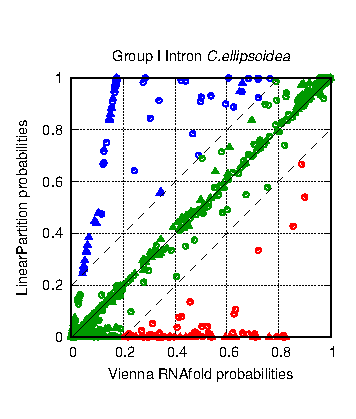
\includegraphics[width=4.4cm]{figs/prob_xy_grp1}}
	  \hspace{-4.5cm}
	   %\raisebox{0cm}
	  {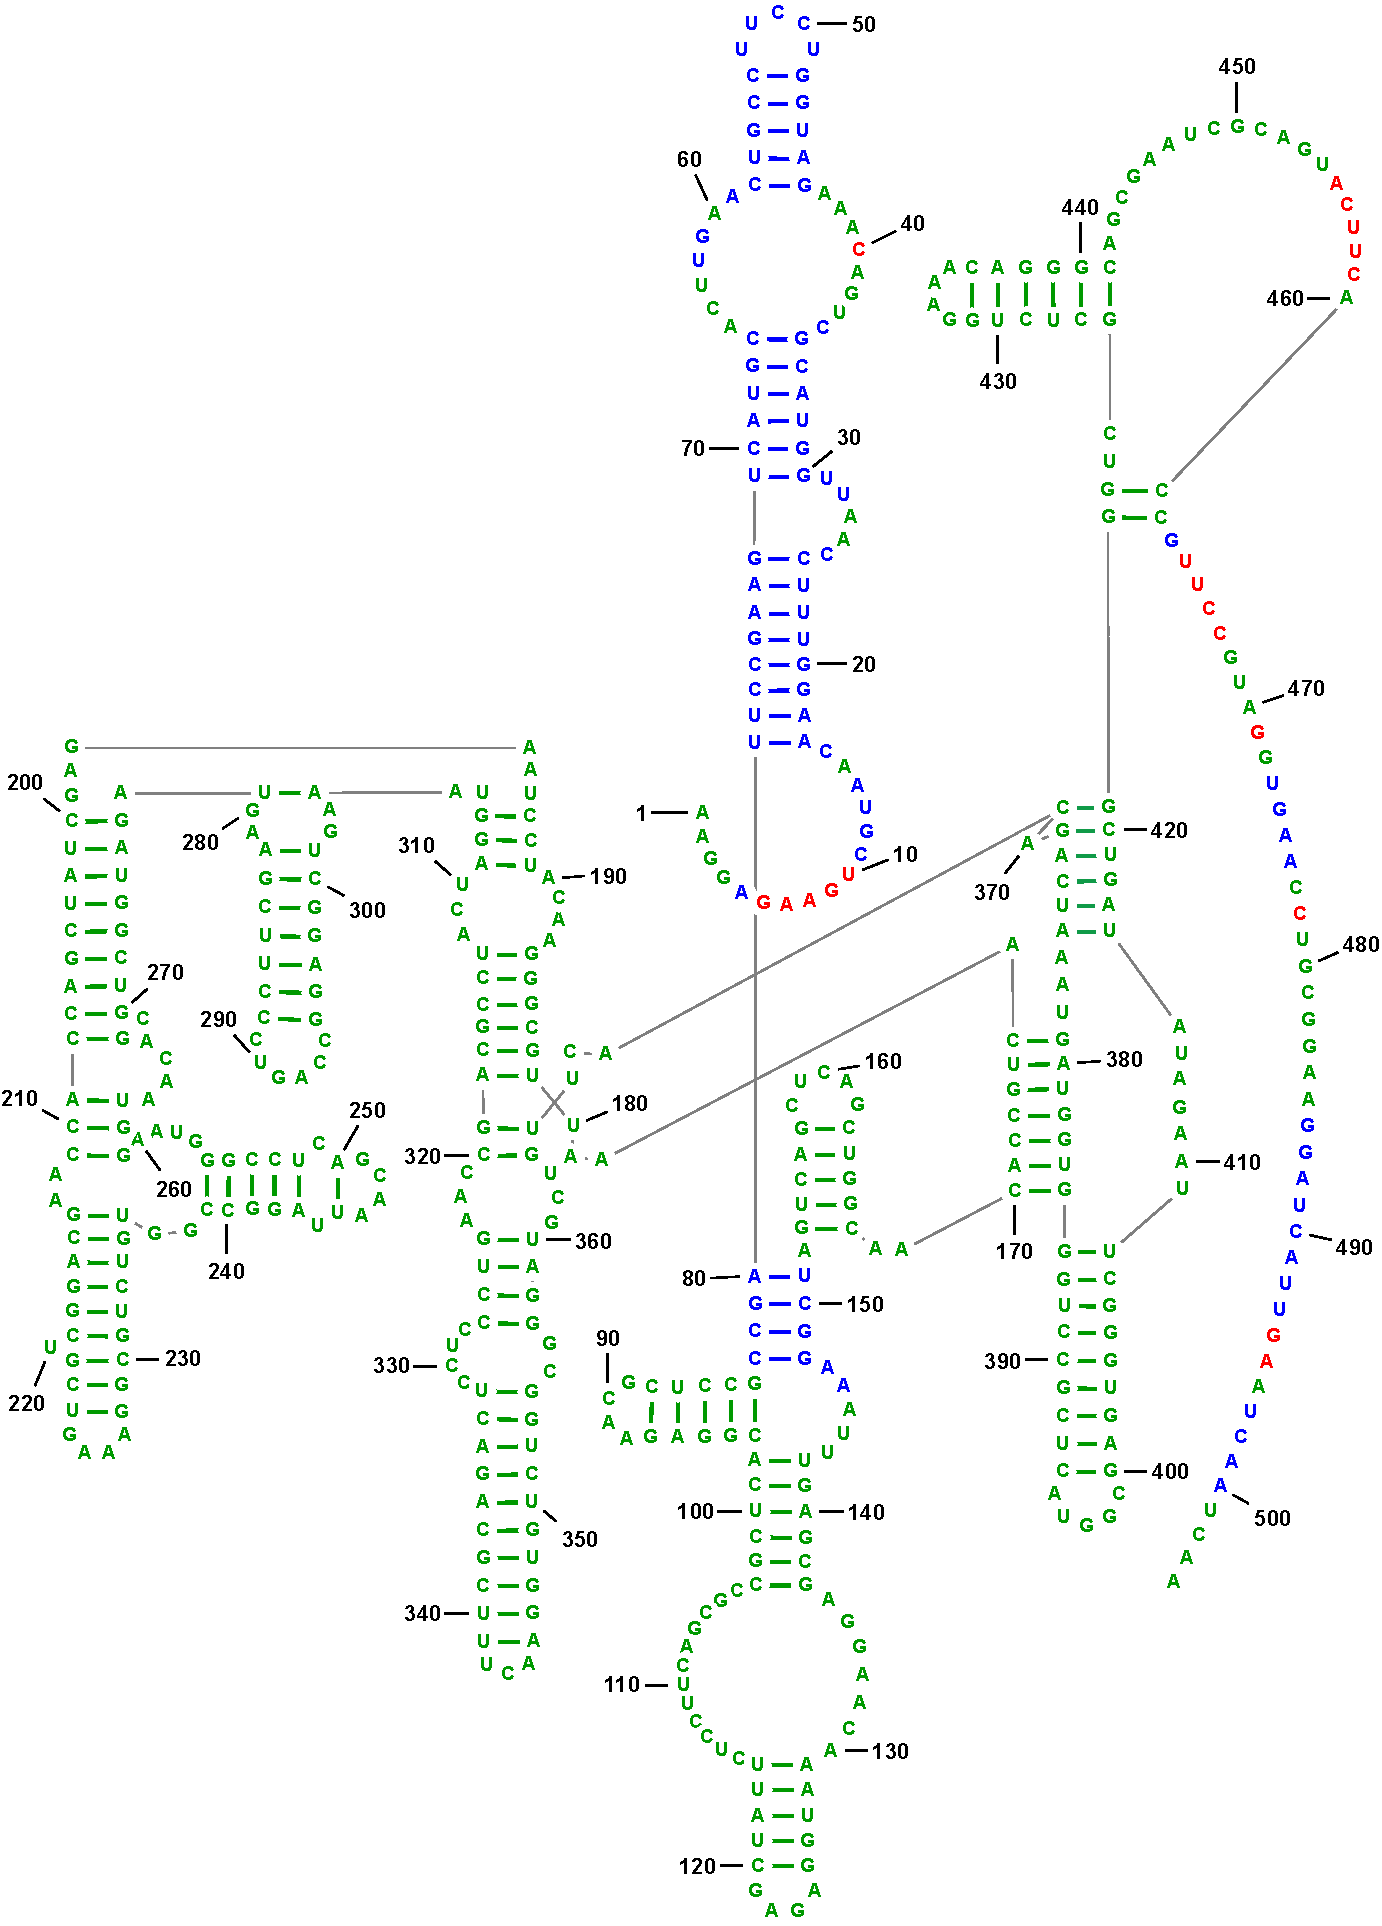
\includegraphics[width=0.5\textwidth]{figs/grp1_70_gutell_modified_2020}}
  	} \\[-1.6cm]
  	\hspace{-.0cm}\panel{C} &  \\[-1.cm]
  	\end{tabular}
% \hspace{-7cm}\panel{B} &\\[-.8cm]

% &&\raisebox{0cm}{\hspace{0.2cm}\includegraphics[width=0.25\textwidth]{figs/23s_gold}} \\
% &&\hspace{-4.5cm}\panel{E}\\[-.3cm]
% &&\raisebox{0cm}{\hspace{0.2cm}\includegraphics[width=0.25\textwidth]{figs/23s_vienna_plfold_example}} \\
% &&\hspace{-4.5cm}\panel{F}\\[-.3cm]
% &&\raisebox{0cm}{\hspace{0.2cm}\includegraphics[width=0.25\textwidth]{figs/23s_vienna_example}} \\
% &&\hspace{-4.5cm}\panel{G}\\[-.3cm]
% &&\raisebox{0cm}{\hspace{0.2cm}\includegraphics[width=0.25\textwidth]{figs/23s_example}} \\[-2.3cm]
% % } & \\[-.4cm]
% \hspace{-.2cm}\raisebox{1cm}{\panel{C}} & \\[-2.2cm]
% \hspace{-7cm}\panel{E} &\\[-.5cm]
% \multicolumn{2}{l}{% \hspace{-0.3cm}

\resizebox{0.5\textwidth}{!}
{
  \begin{tabular}{c}
%	\toprule
         % &     \multicolumn{2}{c}{total} & \multicolumn{2}{c}{correct} \\
			 % \midrule
\hspace{6.5cm}{\color{blue} $p_\linear \!-\! p_\vienna \!>\! 0.2$} \\[.3cm]
\hspace{6.4cm}{\color{darkgreen} $|p_\linear \!-\! p_\vienna| \!\leq \!0.2$} \\[.3cm]
\hspace{6.3cm}{\color{red} $p_\linear \!-\! p_\vienna \!<\! -0.2$}  \\[-2.4cm]
%	                 \bottomrule
  \end{tabular}
 }

% \resizebox{0.45\textwidth}{!}
% \panel{C}}
\vspace{.5cm}
{
  \hspace{-4.5cm}\begin{tabular}{r@{\; }r@{\quad}r@{\; }r}
%	\toprule
% \panel{C}} & &&\\
          \multicolumn{2}{c}{total} & \multicolumn{2}{c}{correct} \\
			 \midrule
55 \bluetri & 40 \bluecir  & 23 \bluetri & 37 \bluecir \\
  126,645 \greentri & 420 \greencir & 111 \greentri & 180 \greencir\\
 56 \redtri & 44 \redcir & 0 \redtri & 19 \redcir \\[1.9cm]
%	                 \bottomrule
  \end{tabular}
  }

% }
% &\\[-2cm]
% &\raisebox{5cm}{\hspace{-0.2cm}\includegraphics[width=0.25\textwidth]{figs/23s_gold}} \\
% \end{tabular}\\

% \begin{tabular}{cccc}
% \hspace{-4.4cm} \panel{F} & \hspace{-4.6cm}\panel{G} & \hspace{-4.6cm}\panel{H} & \hspace{-4.6cm}\panel{I}\\[-0.2cm]
% \hspace{-0.2cm}\includegraphics[width=0.25\textwidth]{figs/23s_gold} &
% \hspace{-0.35cm}\includegraphics[width=0.25\textwidth]{figs/23s_vienna_plfold_example.pdf} &
% \hspace{-0.35cm}\includegraphics[width=0.25\textwidth]{figs/23s_vienna_example} &
% \hspace{-0.35cm}\includegraphics[width=0.25\textwidth]{figs/23s_example.pdf}
% \end{tabular}
\vspace{-2cm}
\caption{
{\bf A--C}: An example of {\it C.~ellipsoidea} Group I Intron. 
{\bf A}: Solid triangles ({\small {\color{blue} $\blacktriangle$} {\color{darkgreen}$\blacktriangle$}  {\color{red}$\blacktriangle$}}) stand for base pairing probabilities and
unfilled circles ({\small {\color{blue} $\circ$} {\color{darkgreen}$\circ$}  {\color{red}$\circ$}})  stand for single-stranded probabilities.
{\color{blue} blue: $p_\linear \!-\! p_\vienna \!>\! 0.2$};
{\color{darkgreen} green: $|p_\linear \!-\! p_\vienna| \!\leq \!0.2$};
{\color{red} red: $p_\linear \!-\! p_\vienna \!<\! -0.2$};
%some high probability pairs and unpaired bases in \linearpartition have low probabilities in \viennarnafold (in blue), and some low probability ones in \linearpartition have high probabilities in \viennarnafold (in red); 
	{\bf B}: Ground truth structure colored with the above scheme; % from \viennarnafold and \linearpartition; 
	%pink binds around position 370 are pseudoknotted pairs.
	{\bf C}: Statistics of this example. 
	"total" columns are the total numbers of triangles and circles with different colors in {\bf A},
	while "correct" columns are the corresponding numbers %of such triangles and circles
        in the ground-truth structure  in {\bf B},
        which is better correlated with \linearpartition's probabilities than \viennarnafold's ({\color{blue} 23 blue pairs} and {\color{red} 0 red pairs}). %ground-truth structure.
	% Note that each triangle represents a pair of nucleotides.
%% {\bf D--G}: An example of \ecoli 23S rRNA. 
%% 	{\bf D}: circular plot of the ground truth.
%% {\bf E--G}: circular plots using the base pair probabilities from \viennarnaplfold (with default window size $70$), \rnafold and \linearpartition, respectively; 
%% base pairs in the ground truth are in blue;
%% the color shade of the lines are propotional to their probabilities.
	\label{fig:example}\\[-.7cm]
}
\end{figure}


\begin{figure*}[hbt!]
\center
\begin{tabular}{@{}c@{}c@{}c@{}c@{}}
\hspace{-4.6cm}\panel{A} & \hspace{-5.2cm}\panel{B} & \hspace{-5.2cm}\panel{C} & \hspace{-2.3cm}\panel{D} 
\\[-0.6cm]
\raisebox{0.35cm}{\includegraphics[scale=.8]{figs/LP_MEA_curves}} 
&
%\hspace{-0.5cm}
\hspace{-0.3cm}\includegraphics[scale=.93]{figs/MEA_vs_MFE_PPV} 
&
%\hspace{-0.5cm}
\hspace{-0.2cm}\includegraphics[scale=.93]{figs/MEA_vs_MFE_sens}  
&
\raisebox{.5cm}{\hspace{0.2cm}\includegraphics[scale=.56]{figs/bylen_500_mea}}
\\[-0.5cm]
\hspace{-4.6cm}\panel{E} & \hspace{-5.2cm}\panel{F} & \hspace{-5.2cm}\panel{G} & \hspace{-2.3cm}\panel{H} 
\\[-0.5cm]
\raisebox{0.35cm}{\includegraphics[scale=.8]{figs/LP_ThreshKnot_curves.pdf}}
&
%\hspace{-0.5cm}
       \hspace{-0.3cm}{\includegraphics[scale=.93]{figs/new_ThreshKnot_vs_MFE_PPV}}
&
%       \hspace{-0.5cm}
      \hspace{-0.2cm}{\includegraphics[scale=.93]{figs/new_ThreshKnot_vs_MFE_sens}}
              &
\raisebox{.5cm}{\hspace{0.3cm}\includegraphics[scale=.56]{figs/bylen_500_threshknot} }
\vspace{-0.6cm}
\end{tabular} % A: specify MFE in label
\caption{Accuracy of downstream  predictions (MEA and \threshknot) using base pairing probabilities from \viennarnafold and \linearpartition
        on the ArchiveII dataset.
	{\bf A}: Overall PPV-Sensitivity tradeoff of MFE (single point) and MEA with varying $\gamma$
	%MFE is a single point, but
        (which can be tuned for higher sensitivity or PPV by adjusting $\gamma$).
	{\bf B} \& {\bf C}: PPV and Sensitivity comparisons of MEA structures for each family.
  {\bf D}: Accuracy comparison of long-distance base pairs (>500 \nts apart) in the MEA structures.
        {\bf E--H}: Same as {\bf A--D}, but using \threshknot predictions instead of MEA.
	%% {\bf D}: Overall PPV-Sensitivity tradeoff of \threshknot with varying threshold $\theta$.
	%% {\bf E} and {\bf F}: PPV and Sensitivity comparisons of ThreshKnot structures for each family.
        %	For easy comparison, {\bf A} and {\bf D} and also {\bf BCEF} are on the same scales.
        We conclude that MEA predictions based on \linearpartitionv are consistently better in both PPV and Sensitivity than
        those based on \viennarnafold for all $\gamma$'s,
        while \threshknot predictions based on those two are almost identical for all $\theta$'s.
        \linearpartitionv is  substantially better on long-distance base pairs in both MEA and \threshknot predictions.
	\label{mea}
        \vspace{-0.6cm}
}
\end{figure*}


Fig.~\ref{fig:ensemble}A--B employs ensemble defect to measure 
the average number %(Fig.~\ref{fig:ensemble_defect}A) 
%and ratio %(Fig.~\ref{fig:ensemble_defect}B) 
of incorrectly predicted nucleotides over the whole ensemble (lower is better).
% ~\cite{Dirks+:2004, Zadeh+:2010}.
\viennarnafold and \linearpartition have similar ensemble defects for short sequences, % are mostly similar between , % are the same or similar,
but \linearpartition has lower ensemble defects for longer sequences, esp.~16S and 23S rRNAs;
in other words, \linearpartition's ensemble has less expected number of incorrectly predicted nucleotides
(or higher number of correctly predicted nucleotides). %, i.e., better correlation with ground-truth structure).
In particular, on 16S and 23S rRNAs, \linearpartition has on average 15.9 and 56.3 more correctly predicted nucleotides than \rnafold,
and on average 8.3 more correctly predicted nucleotides over all families (Fig.~\ref{fig:ensemble}B).
Figs.~\ref{fig:ensemble_defect} show the relative ensemble defects (normalized by sequence lengths),
where the same observations hold, and \linearpartition has on avearge 0.4\% more correctly predicted nucleotides over all families.
In both cases, the differences on tmRNA (worse) and Group I Intron (better) are statistically significant ($p<0.01$).



This finding also implies that  \linearpartition's  base pairing probabilities 
are on average higher than \rnafold's for ground-truth base pairs,
and on average lower for incorrect base pairs.
We use two concrete examples to illustrate this.
First, we plot the ground truth structure of \ecoli 23S rRNA (2,904~\nts) in
Fig.~\ref{fig:ensemble}C,
and then plot the predicted base pairing probabilities
from the local folding tool \viennarnaplfold (with default window size 70), \rnafold, and \linearpartition
in Fig.~\ref{fig:ensemble}D--F, respectively.
We can see that local folding can only produce local pairing probabilities,
while \rnafold misses
most of the long-distance pairs from the ground truth (except the 5'-3' helix),
and includes many incorrect long-distance pairings (shown in red).
By contrast, \linearpartition successfully predicts many
long-distance pairings that \rnafold misses, the longest being 582~\nts apart (shown with arrows).
Indeed, the ensemble defect of this example confirms that \linearpartition's ensemble distribution
has on average 211.4 more correctly predicted nucleotides (over 2,904~\nts, or 7.3\%) than \rnafold's.

As the second example, we use %an RNA sequence,
{\it C.~ellipsoidea} Group I Intron (504~\nts).
First, in Fig.~\ref{fig:ensemble}G--J, we plot the circular plots in the same style as the previous example,
where \linearpartition is substantially better in predicting 4 helices in the ground-truth structure:
[17,24]--[72,79], [30,45]--[66,71], [44,48]--[54,58], and [80,83]--[148,151] (annotated with blue arrows).
%as an example to illustrate this.
% show \linearpartition gives more accurate predicted secondary structure than \viennarnafold.
%compare the base pairing probabilities generated by \viennarnafold and \linearpartition.
Next, in Fig.~\ref{fig:example}A, 
we plot the base pairs (in triangle) and unpaired bases (in circle) 
with \rnafold probability on x-axis and \linearpartition probability on y-axis.
We color the circles and triangles in blue where \linearpartition gives 0.2 higher probability 
than \rnafold %gives low probabilities 
(top left region),
the opposite ones (bottom right region) in red,
and the remainder (diagonal region, with probability changes less than 0.2)
in green.
Then in Fig.~\ref{fig:example}B,
we visualize the ground truth structure~\cite{Cannone+:2002} and color the bases as in Fig.~\ref{fig:example}A.
We observe that the majority of bases are in green, indicating that \rnafold and \linearpartition
agree  with for a majority of the structure features. 
But the blue helices (near 5'-end and [80,83]--[148,151], see also Fig.~\ref{fig:ensemble}J)
indicate that \linearpartition favors these correct substructures by giving them higher probabilities than \rnafold.
We also notice that all red features (where \rnafold does better than \linearpartition) are unpaired bases.
This example shows that although \linearpartition and \rnafold give different probabilities, % compared with \rnafold, 
it is likely that \linearpartition prediction structure is closer to the ground truth structure
(which will be confirmed by downstream structure predictions in Section~\ref{sec:acc}).
The ensemble defect of this example also confirms
that \linearpartition has on average 47.1 more correctly predicted nucleotides (out of 504~\nts, or 9.3\%)
than \rnafold.




Fig.~\ref{fig:example}C gives the statistics of this example.
We can see the green triangles in Fig.~\ref{fig:example}A, 
which denote similar %base pairing
probabilities between \rnafold and \linearpartition, 
are the vast majority. % and the total number is 126,645.
The total number of blue triangles,
for which \linearpartition gives higher base pairing probabilities,
is 55,
and among them 23 %base pairs
(41.8\%) are in the ground truth structure.
On the contrary,
56 triangles are in red,
but none of these \rnafold prefered base pairs are correct. %in the ground truth structure.
% Notice that all the red triangles are on $y=0$ line, 
% for which \linearpartition gives 0 probabilities,
% are in the ground truth structure.
For unpaired bases, 
\linearpartition also gives higher probabilities to more ground truth unpaired bases:
there are 40 blue circles,
among which 37 (92.5\%) are unpaired in the ground truth structure,
while only 19 out of the 44 red circles (43.2\%) are in the ground truth structure.
%% See also Fig.~\ref{fig:ensemble}G--J for another view of this example in the style of Fig.~\ref{fig:ensemble}C--F
%% using circular plots.


\vspace{-0.3cm}
\subsection{Accuracy of Downstream Predictions}%  using Base Pairing Probabilities}
\label{sec:acc}


% \begin{figure}[t!]
% \center
% \begin{tabular}{cc}
% \raisebox{2cm}{\panel{A}} & \includegraphics[scale=.7]{figs/new_MEA_diff_gamma_beam_inf_threshold_001} \\[-0.6cm]
% \raisebox{2cm}{\panel{B}} &
% \raisebox{-0.25cm}{\includegraphics[scale=.58]{figs/for_He_Zhang_MEA_gamma_B100}}\\[-0.6cm]
% \raisebox{3cm}{\panel{C}} & \hspace{-0.5cm}\includegraphics[scale=.78]{figs/ProbKnot_PPV}\\[-0.4cm]
% \raisebox{3cm}{\panel{D}} &\hspace{-0.5cm}\includegraphics[scale=.78]{figs/ProbKnot_Sens}

% \end{tabular} % A: specify MFE in label
% \caption{Accuracy comparison for two systems.
% 	{\bf A}: Overall MFE and MEA structure PPV-sensitivity tradeoff of two systems with varying $\gamma$. 
% 	{\bf B}: Overall ThreshKnot structure PPV-sensitivity tradeoff of two systems with varying threshold $p$.
% 	{\bf C-D}: PPV and sensitivity comparison for each family.
% 	\label{mea}
% }
% \end{figure}

An important application of the partition function
is to improve structure prediction accuracy (over MFE) using base pairing probabilities.
%These downstream prediction methods include MEA\cite{do+:2006}, \centroidfold~\cite{sato+:2009}, \dotknot~\cite{Sperschneider+Datta:2010}, \probknot~\cite{bellaousov+mathews:2010}, and \ipknot~\cite{sato+:2011},
%have been shown to outperform MFE in accuracy
Here we use two such ``downstream prediction'' methods, MEA\cite{do+:2006} and \threshknot~\cite{Zhang+:2019} which is a thresholded version of \probknot~\cite{bellaousov+mathews:2010},
and compare their results using base pairing probabilities from $O(n^3)$-time baselines and our $O(n)$-time \linearpartition.
%We next consider the accuracy of downstream structure prediction using \linearpartition-produced 
%% First we take base pairing probability matrices from \linearpartition and \viennarnafold (or \contrafold), 
%% feed them to the standard MEA algorithm separately, 
%% and compare the accuracies of prediction structures.
We use Positive Predictive Value (PPV, the fraction of predicted pairs in the known structure, a.k.a.~precision) 
and sensitivity (the fraction of known pairs predicted, a.k.a.~recall) 
as accuracy measurements for each family,
and get overall accuracy be averaging over families. 
% We use slipping method{}
When scoring accuracy, we allow base pairs to differ by one nucleotide in position~\cite{mathews+:1999}.
% ~\cite{sloma+mathews:2016}
We compare \rnafold and \linearpartitionv on the ArchiveII dataset in the main text, and provide the \contrafold vs.~\linearpartitionc comparisons
in the Supporting Information Figs.~\ref{fig:mea_lpc}--\ref{fig:threshknot_lpc}.


% Fig.~\ref{mea} shows that \linearpartition even leads to a small improvement in the downstream MEA predictoin using the probability matrix computed in linear time. 
% Fig.~\ref{mea} gives the accuracy comparison between 
Fig.~\ref{mea}A shows  
MEA predictions (\rnafold + MEA and \linearpartition + MEA) are more accurate than MFE ones (\rnafold MFE and \linearfoldv),
but more importantly,
\linearpartition + MEA  consistently outperforms \rnafold + MEA in both PPV and sensitivity
with the same $\gamma$, a hyperparameter that balances PPV and sensitivity in MEA algorithm.
%\linearpartition + MEA enjoys a small improvement in both PPV and sensitivity.

Figs.~\ref{mea}B--C detail the per-family PPV and sensitivity, respectively,
for MFE and MEA ($\gamma=1.5$) results from Fig.~\ref{mea}A.
% two MFE-based systems and two MEA-based systems for each family
%% for MEA and MFE structures using \rnafold and our \linearfold and \linearpartition.
%% % We can see
%% The MEA
%% % -based systems lead to accuracy improvements over MFE-based systems 
%% structure predictions are more accurate than MFE predictions
%% for most families.
\linearpartition + MEA has similar PPV and sensitivity as \rnafold + MEA on short families (tRNA, 5S rRNA and SRP),
but interestingly, is more accurate on longer families, especially the two longest ones, 16S rRNA (+0.86 on PPV and +1.29 on sensitivity) 
and 23S rRNA (+0.88 on PPV and +0.62 on sensitivity). 
%% We also performed a two-tailed permutation test to test the statistical significance, 
%% and observed that on tmRNA the MEA structures of \linearpartition is significantly worse ($p<0.01$) than \viennarnafold in both PPV and Sensitivity.



% ThreshKnot
%% ProbKnot is another partition function-based structure prediction method that adds a straightforward post-processing step 
%% % after partition function calculation
%% of base pairing probabilities to predict structures
%% and is simpler and faster than MEA~\cite{bellaousov+mathews:2010}.
% Beyond nested structures, ProbKnot can predict pseudoknots. 
\probknot is another downstream prediction method
that is simpler and faster than MEA;
it assembles 
%In ProbKnot, structures are composed of
base pairs with reciprocal highest pairing probabilities. 
Recently, we demonstrated \threshknot~\cite{Zhang+:2019}, 
a simple thresholded version of ProbKnot that only includes pairs that exceed the threshold, 
leads to more accurate %overall 
predictions that outperform MEA by filtering out unlikely pairs, i.e., those whose probabilities fall under a given threshold $\theta$.
%% It has been shown ThreshKnot can achieve better PPV and Sensitivity than the more involved MEA algorithm, 
%% % and can predict pseudoknots which is beyond MEA scope,
%% so we also compare ThreshKnot structure accuracy between \viennarnafold and \linearpartition.


Shown in Fig.~\ref{mea}E, \linearpartition + \threshknot is almost identical in overall accuracy %(slightly better in sensitivity)
to \rnafold + \threshknot at all $\theta$'s,
% in the downstream ThreshKnot prediction using the probability matrix computed in linear time.
%Figs.~\ref{mea}E and F show that \linearpartition + ThreshKnot
and is slightly better than the latter on long families
(+0.24 on PPV and +0.38 on sensitivity for Group I Intron, +0.12 and +0.37 for telomerase RNA, and +0.74 and +0.62 for 23S rRNA)
(Figs.~\ref{mea}F--G).
We also performed a two-tailed permutation test to test the statistical significance, 
and observed that on tmRNA, both MEA and \threshknot structures of \linearpartition are significantly worse ($p\!<\!0.01$) than their \rnafold-based counterparts in both PPV and Sensitivity.
%As was observed for MEA comparison, \linearpartition + ThreshKnot is significantly worse ($p<0.01$) than \viennarnafold on tmRNA.
%in PPV and Sensitivity.


\begin{figure}%[!b]
  \vspace{-.1cm}
\center
%% \iffalse
%% \begin{tabular}{cc}
%% \raisebox{4.6cm}{\panel{A}} & \hspace{-1cm}\includegraphics[width=0.3\textwidth]{figs/ensemble_xy} \\
%% % \raisebox{3.6cm}{\panel{B}}
%% \hspace{-1cm}\includegraphics[width=0.2\textwidth]{figs/ensemble_len}
%%  & \hspace{-1cm}\includegraphics[width=0.2\textwidth]{figs/ensemble_len_norm} \\[-0.3cm]
%% \end{tabular}
%% \fi
%% \iffalse
%% \begin{tabular}{ccc}
%% {\panel{A}} & {\panel{B}} & {\panel{C}} \\
%% \hspace{-1cm}\includegraphics[width=0.3\textwidth]{figs/ensemble_xy} &
%% \hspace{-.8cm}\includegraphics[width=0.3\textwidth]{figs/ensemble_len} &
%% \hspace{-.8cm}\includegraphics[width=0.3\textwidth]{figs/ensemble_len_norm} \\[-0.3cm]
%% \end{tabular}
%% \fi
\begin{tabular}{cc}
% {\panel{A}} & {\panel{B}}\\
\hspace{-0.2cm}\raisebox{2.9cm}{\panel{A}\hspace{-2.2cm}}\raisebox{2.5cm}{\multirow{2}{*}{\includegraphics[width=0.47\textwidth]{figs/ensemble_xy}}} & 
\hspace{-2.4cm}\raisebox{2.9cm}{\panel{B}}\hspace{-.35cm}\includegraphics[scale=0.74]{figs/ensemble_len} \\[-.5cm]
% &{\panel{A}}\\
&\hspace{-2.4cm}\raisebox{2.6cm}{\panel{\color{white}C}}\hspace{-.3cm}\includegraphics[scale=0.79]{figs/ensemble_len_norm} \\[-0.4cm]
\end{tabular}
\caption{
  Approximation quality of partition function  on ArchiveII dataset and random sequences. %. shorter than 3,000~\nts.
  {\bf A}: The x and y axes are
  ensemble folding free energy changes $\ensenergy(\vecx)$ of \viennarnafold %($-RT\log Q_\vienna(\vecx)$)
  and \linearpartition, % ($-RT\log Q_\linear(\vecx)$),
  respectively.
  {\bf B}: 
  Difference of ensemble folding free energy change (top), ${\ddg(\vecx)}$, between \rnafold and \linearpartition.
  and the relative differences (bottom),  ${\ddg(\vecx)}/{\ensenergyvienna(\vecx)}$, in percentages.
  %% of 
  %% ensemble folding free energy changes,
%  $\frac{ \ensenergyvienna(\vecx) - \ensenergylinear(\vecx)}{\ensenergylinear(\vecx)}$.
  \label{fig:partition}
  \vspace{-0.2cm}
}
\end{figure}


Fig.~\ref{mea}D \& H show that \linearpartition-based predictions are subtantially better than \rnafold's (in both PPV and sensitivity) for long-distance base pairs (those with 500+ \nts apart),
which are well known to be challenging for the current models.
Fig.~\ref{fig:distance} details the accuracies on base pairs with different distance groups.


Figs.~\ref{fig:mea_lpc}--\ref{fig:threshknot_lpc} show similar comparisons between 
\contrafold and \linearpartitionc using MEA and ThreshKnot prediction, %, separately. 
% Fig.~\ref{fig:mea_lpc} compares MEA structures ($\gamma>1.5$) accuracy based on these two systems and Fig.~\ref{fig:threshknot_lpc} compares ThreshKnot structures ($p>0.2$). 
with similar results to Fig.~\ref{mea}, i.e., downstream structure prediction using \linearpartitionc is as accurate as using \contrafold, and  (sometimes significantly) more accurate on longer families.


\iftrue
%<<<<<<< HEAD
\begin{figure*}[!h]
%\vspace{-0.2cm}
%% =======
%% \begin{figure*}[!ht]
%% \vspace{-0.5cm}
%% >>>>>>> e07b35b96f33f564a07e21f062362ad3acd7bbad
\center
\begin{tabular}{cc|c}
\hspace{-5.5cm}\panel{A} & \hspace{-6.cm}\panel{B} & \hspace{-5.2cm}\panel{E} \\[-0.5cm]
\hspace{-0.5cm}\includegraphics[width=0.33\textwidth]{figs/tRNA_identical_heatmap}
&
% \hspace{-0.8cm}{\includegraphics[width=0.33\textwidth]{figs/rmsd_family_plus_random_b2}}
\hspace{-1.1cm}{\includegraphics[width=0.33\textwidth]{figs/rmsd_archiveII_rnacentral_lpv_float_plus_long_random}}
% \\[-0.2cm]
&
% \panel{C} & \panel{D}\\[-0.5cm]
\hspace{0.2cm}\includegraphics[width=0.33\textwidth]{figs/overall_average_change_prob} \\[-0.1cm]

\hspace{-5.5cm}\panel{C} & \hspace{-6.cm}\panel{D} & \hspace{-5.2cm}\panel{F} \\[-0.5cm]
\hspace{-.8cm}\raisebox{-0.2cm}{\includegraphics[width=0.35\textwidth]{figs/structure_entropy_xy_plus_random_rnacentral}}
&
\hspace{-0.7cm}\includegraphics[width=0.33\textwidth]{figs/sorted_prob_23s} 
&
\hspace{-0.0cm}\includegraphics[width=0.34\textwidth]{figs/overall_vienna_prob_bin_count}  \\[-0.2cm]
\end{tabular}
\caption{
Comparison of base pairing probabilities from \viennarnafold and \linearpartition.
	{\bf A}: \linearpartition (upper triangle) and Vienna RNAfold (lower triangle) result in identical base pairing probability matrix for \ecoli tRNA$^\textit{Gly}$.
	{\bf B}: The root-mean-square deviation, $\RMSD(p_\vienna, p_\linear)$, is relatively small between \linearpartition and Vienna RNAfold; all tRNA and 5S rRNA sequences \RMSD is close to 0 (e.g., RMSD$<10^{-5}$).
	{\bf C}: Average positional structural entropy $H(p)$ comparison; \linearpartition has noticeably lower entropy.
	{\bf D}: \linearpartition starts higher and finishes lower than \viennarnafold in a sorted probability curve for \ecoli 23S rRNA,
        suggesting lower entropy.
	{\bf E}: Mean absolute value of change in base pairing probabilities between \viennarnafold and \linearpartition; these changes are averaged within every probability bin.
	{\bf F}: Pair probability distribution of \viennarnafold. 
	Note that the y-axis is limited to 50,000 counts, and the counts of first three bins (with probability smaller than 3\%) are far beyond 50,000.
	\label{fig:rmsd}
}
\vspace{-0.3cm}
\end{figure*}
\fi



\vspace{-0.2cm}
\subsection{Approximation Quality (Default Beam Size)}

\linearpartition uses beam pruning to ensure $O(n)$ runtime, % and linear space, % linearity, 
thus is approximate compared with standard $O(n^3)$-time algorithms.
% Fig. 4A–B show that our \linearpartition algorithm can indeed approximate the partition function reasonably well.
We now investigate its approximation quality at the default beam size~100.

First, in Fig.~\ref{fig:partition}, we measure the approximation quality of the partition function calculation,
%and specifically,
in particular,  the ensemble folding free energy change (also known as ``free energy of the ensemble'')
which reflects the size of the partition function, 
\[
\ensenergy (\vecx) = -RT \log Q(\vecx).
\]
Fig.~\ref{fig:partition}A shows that the \linearpartition 
% free energy of ensemble 
estimate for the ensemble folding free energy change
is close to the \rnafold estimate 
on the ArchiveII dataset and randomly generated RNA sequences.
The similarity shows that little magnitude of the partition function is lost by the beam pruning. 
For short families, free energy of ensembles between \linearpartition and \rnafold are almost the same.
For 16S and 23S rRNA sequences and long random sequences (longer than 900 nucleotides), 
\linearpartition gives a lower magnitude ensemble free energy change, 
but the difference,
\[
\ddg(\vecx) = \ensenergyvienna(\vecx) - \ensenergylinear(\vecx) \, \geq 0
\]
is smaller than 20 kcal/mol for 16S rRNA, 
15 kcal/mol for 23S rRNA,
and 37 kcal/mol for random sequences (Fig.~\ref{fig:partition}B). 
The maximum difference for random sequence is larger than natural sequences (by 17.2 kcal/mol).
This likely reflects the fact that random sequences tend to fold less selectively to probable structures~\cite{Fu+:2015},
and the beam is therefore pruning structures in random that would contribute to the overall folding stability.
% Fig.~\ref{ensemble} confirms \linearpartition approximation quality of partition function is good.
Fig~\ref{fig:partition}C shows the ``relative'' differences in ensemble free energy changes,
 ${\ddg(\vecx)}/{\ensenergyvienna(\vecx)}$,
are also very small: only up to 2.5\% and 1.5\% for 16S and 23S rRNAs, and up to 4.5\% for random sequences.



Next, in Fig.~\ref{fig:rmsd}, we measure the approximation quality of base pairing probabilities using root-mean-square deviation (\RMSD)
between two probability matrices $p$ %(from cubic algorithms, for example, \viennarnafold) 
and $p'$ %(from our algorithm, for example, \linearpartition)
%(i.e., $p_\vienna$ and $p_\linear$)
over the set of all possible Watson-Crick and wobble pairs on a sequence $\vecx$.
We  define
\begin{equation}
  \vspace{-0.4cm}
\begin{split}
  {\pairings}(\vecx) \!=\!\{  &1\leq i <j\leq |\vecx| \bigm\vert j-i>3 \\[-0.1cm]
    &  \vecx_i\vecx_j \in \{\text{\small CG, GC, AU, UA, GU, UG}\}\!\} \notag
\end{split}
\end{equation}
\vspace{-0.2cm}
and:\vspace{-0.05cm} 
\begin{equation}
\RMSD(p,p')\!=\!\!\!\sqrt{\frac{1}{|{\pairings}(\vecx)|} \sum_{(i,j) \in {{\pairings}(\vecx)}}{\!\!\!\!\!(p_{i,j}\!-\!p'_{i,j})}^2}\notag
\end{equation}

\begin{figure*}[!h]
  \vspace{-0.7cm}
\center
\begin{tabular}{cccc}
% \hspace{-5.cm} \panel{A} & \hspace{-5.2cm}\panel{B}  \\[-0.2cm]
\raisebox{3.7cm}{\panel{A}} & 
\hspace{-0.5cm}\includegraphics[width=0.4\textwidth]{figs/ensemble_beamsize_overall} &
\raisebox{3.7cm}{\panel{B}} &
\hspace{-0.5cm}{\includegraphics[width=0.4\textwidth]{figs/RMSD_beamsize_overall}}
\end{tabular}
\\[-1.2cm]
\begin{tabular}{c@{}c@{}c@{}c@{}c@{}c}
% \hspace{-5.cm}\panel{C} & \hspace{-5.2cm}\panel{D} & \hspace{-5.8cm}\panel{E} \\[-0.2cm]
\hspace{0.6cm}\raisebox{3.8cm}{\panel{C}} & 
\hspace{-1cm}\includegraphics[width=.35\textwidth]{figs/precision-recall-overall-lpv} 
&
\hspace{-.5cm}\raisebox{3.8cm}{\panel{D}} & 
\hspace{-1.2cm}\includegraphics[width=0.35\textwidth]{figs/precision-recall-tmRNA-lpv-hzhang}
&
\hspace{-0cm}\raisebox{3.8cm}{\panel{E}} & 
\hspace{-1.5cm}\includegraphics[width=0.35\textwidth]{figs/precision-recall-16s-lpv-hzhang}
\vspace{-0.4cm}
\end{tabular}
\caption{
Impact of beam size. 
{\bf A}: Relative difference of 
  ensemble folding free energy change, $\ddg/\Delta G^\circ_\text{ensemble}$, against  beam size. %, averaged over all families.
{\bf B}: RMSD against beam size. %, averaged over all families.
{\bf C}: Overall PPV and Sensitivity with beam size.
{\bf D--E}: tmRNA and 16S rRNA PPV and Sensitivity against beam size, respectively. 
%{\bf E}: 16S rRNA PPV and Sensitivity change with beam size. 
Note that the  results of \threshknot using \rnafold (yellow triangles in {\bf C--E}) are identical to \threshknot using
the {\em exact} version of \linearpartition ($b\!=\!\infty$).
%since \linearpartition with infinite beam size (i.e., no beam pruning) does $O(n^3)$ exact partition function calculation as \viennarnafold.
\label{fig:beamsize}
\vspace{-0.7cm}
}
\end{figure*}


Figs.~\ref{fig:rmsd}A and B confirm that our \linearpartition algorithm (with default beam size 100) can indeed approximate the base pairing probability matrix reasonably well. 
Fig.~\ref{fig:rmsd}A shows the heatmap of probability matrices for {\it E.~coli} tRNA$^\textit{Gly}$. 
\rnafold (lower triangle) and \linearpartition (upper triangle)
yield identical matrices (i.e., $\RMSD=0$). % (i.e., RMSD$\approx$0). 
Fig.~\ref{fig:rmsd}B shows that the \RMSD of each sequence in ArchiveII and RNAcentral datasets, 
and randomly generated artificial RNA sequences, %with length 100–16,000~\nts.
is relatively small. % across all sequences. 
% To verify approximation quality of 
The highest deviation is 0.065 for {\it A.~truei} RNase P RNA, 
which means on average 
each base pair's probability deviation in that worst-case sequence is about 0.065 between the cubic algorithm (\rnafold) and our linear-time one (\linearpartition). 
On the longest 23S rRNA family, the \RMSD is about 0.015. 
We notice that tmRNA is the family with biggest average \RMSD. %, and its accuracy is also the worst.
The random RNA sequences behave similarly to natural sequences in terms of \RMSD, 
i.e., \RMSD is  close to 0 ($\!<\!10^{-5}$) for short ones, then becomes bigger around length 500 and decreases after that, 
but for most cases their \RMSD's are slightly larger than  
the natural sequences. %in similar length range.
This indicates that the approximation quality is relatively better for natural sequences.
For RNAcentral-sampled sequences, \RMSD's are all small and around 0.01.

% With sequence length increasing, RMSD gradually decreases, 
% since the number of possible pairs grows in $O(n^2)$ but the number of highly probable pairs grows in $O(n)$. 
% To avoid RMSD is dominented by most base pairs with small probabilities,
% we consider a more strict circumstance. 
% Instead of divided by the number of all possible base pairs,
% We only consider the ones which have probability $p>0.01$.
% The RMSD resutls with such constrain are presented in Fig.~\ref{fig:rmsd_threshold}.
% It shows that for sequence shorter than 300$nt$, RMSD($p>0.01$) is still 0. 
% This also confirms that our \linearpartition gives exactly the same probability matrix as cubic algorithm.
% RMSD($p>0.01$) fluctuates from 0 to about 0.43 for sequences whose lengthes are in the range [300,1000]. Beyond 1,000$nt$, RMSD($p>0.01$) becomes stable between 0.2 and 0.4.



% Fig.~\ref{fig:rmsd}C and D show
We hypothesize that \linearpartition reduces the uncertainty of the output  distributions %(both base pairing probabilities distribution
%is shifted to higher probability 
because it filters out states with lower partition function.
We measure this using average positional structural entropy $H(p)$, %$~\cite{Garcia-Martin+Clote:2015}, 
% which is defined as:
which is the average of positional structural entropy $H_2(i)$ for each nucleotide $i$~\cite{Huynen+:1997,Garcia-Martin+Clote:2015}:
\vspace{-0.2cm}
\begin{equation}
  \vspace{-0.3cm}
\begin{split}
H(p) &= \frac{1}{n}\sum_{i=1}^{n}{H_2(i)} =\frac{1}{n}\sum_{i=1}^{n}({-\sum_{j=0}^{n}p_{i,j}\mathrm{log}_{2}p_{i,j}}) \\
		&=-\frac{1}{n}\sum_{i=1}^{n}{\sum_{j=0}^{n}p_{i,j}\mathrm{log}_{2}p_{i,j}} \notag
\end{split}
\end{equation}
where $p$ is the base pairing probability matrix,
% in which 
%$p_{i,j}$ is the probability of nucleotide $i$ paired with $j$ when $j\neq 0$, 
and $p_{i,0}$ is the probability of nucleotide $i$ being unpaired ($q_i$ in Eq.~\ref{eq:phi}).
%$n$ is the sequence length.
The lower entropy indicates that the distribution is dominated by fewer base pairing probabilities.
Fig.~\ref{fig:rmsd}C confirms \linearpartition distribution shifted to higher probabilities (lower average entropy) than \rnafold for most sequences.

Fig.~\ref{fig:rmsd}D uses \ecoli 23S rRNA to exemplify the difference in base pairing probabilities.
We sort all these probabilities from high to low and take the top 3,000.
The \linearpartition curve starts higher and finishes lower, confirming a lower entropy. %the distribution shifts to higher probabilities. % (rich get richer).



% E F
Figs.~\ref{fig:rmsd}E and F follow a previous analysis method~\cite{Zuber+:2017} to estimate the approximation quality with a different perspective. 
We divide the base pairing probabilities range [0,1] into 100 bins, i.e., the first bin is for base pairing probabilities [0,0.01), and the second is for [0.01, 0.02), so on so forth. 
In Fig.~\ref{fig:rmsd}E we visualize the averaged change of base pairing probabilities between \rnafold and \linearpartition for each bin.
We can see that larger probability changes are in the middle (bins with probability around 0.5),
and smaller changes on the two sides (with probability close to either 0 or 1).
%while both on the left (bins with probability near 0) and on the right (bins with probability near 1) the changes are smaller.
In Fig.~\ref{fig:rmsd}F we illustrate the counts in each bin based on \rnafold base pairing probabilities.
We can see that most base pairs have low probabilities (near 0) or very high probabilities (near 1).
Combine Figs.~\ref{fig:rmsd}E and F together, we can see that probabilities of most base pairs are near 0 or 1, where the differences between \rnafold and \linearpartition are relatively small. 
Fig.~\ref{fig:bin_counts} provides the comparison of counts in each bin between \rnafold and \linearpartitionv. The count of \linearpartitionv in bin [99,100) is slightly higher than \rnafold, 
while the counts in bins near 0 (being capped at 50,000) are much less than \rnafold.
This  also confirms that \linearpartition prunes base pairs with tiny probabilities.



\vspace{-0.4cm}
\subsection{Adjustable Beam Size}

Beam size in \linearpartition is a user-adjustable hyperparameter controlling beam prune, 
and it balances the approximation quality and runtime.
A smaller beam size shortens runtime, but sacrifices approximation quality.
With increasing beam size, \linearpartition gradually approaches the classical $O(n^3)$-time algorithm and 
the output is finally identical to the latter when the beam size is $\infty$ (no pruning).
Fig.~\ref{fig:beamsize}A shows the changes in approximation quality of the ensemble free energy change,
$\Delta G^\circ_\text{ensemble}(\vecx)$, with $b=20\rightarrow 800$.
Even with a small beam size ($b=20$) the difference is only about 5\%, which quickly shrinks to 0 as $b$ increases.
Fig.~\ref{fig:beamsize}B shows the changes in \RMSD with changing $b$. %=20\rightarrow 800$.
% We use averaged length and averaged RMSD for each family with a certain beam size.
%We observe that \RMSD decreases when beam size increases. 
With a small beam size $b=20$ the average \RMSD is lower than 0.035
over all ArchiveII sequences,
which shrinks to less than 0.005 at the default beam size ($b=100$),
and almost 0 with $b=500$.% the average \RMSD is
% and tmRNA remains relatively high averaged RMSD compared with other short families.
% This is consistant with Fig.~\ref{fig:rmsd}B.
%% With a larger beam size, $b=500$, 
%% % which means no beam prune for partition function calculation, 
%% the average \RMSD decreases to almost 0.
% It is also clear that shorter families' averaged RMSD decreases faster. 


Beam size also has impact on PPV and Sensitivity.
Fig.~\ref{fig:beamsize}C gives the overall PPV and Sensitivity changes with beam size.
We can see both PPV and Sensitivity improve from $b=50$ to $b=100$,
and then become stable beyond that.
%Therefore, we choose beam size 100 as the default beam size.
Figs.~\ref{fig:beamsize}D and E present this impact for two selected families.
% tmRNA is the worst family in the sense of accuracy for \linearpartition.
Fig.~\ref{fig:beamsize}D shows tmRNA's PPV and Sensitivity both increase when enlarging beam size.
Using beam size 200, \linearpartition achieves similar PPV and Sensitivity as \rnafold.
% This indicates that it is better to use a larger beam size, for example, $b=200$ when running 
% \linearpartition on tmRNA sequence.
However, increasing beam size is not benefical for all families.
% especially for long families.
Fig.~\ref{fig:beamsize}E gives the counterexample of 16S rRNA. 
We can see both PPV and Sensitivity decrease with $b$ from 50 to 100.
After that, Sensitivity drops with no PPV improvement.
% PPV increases while Sensitivity decreases when changing beam size from 100 to 120. 
% Continue increasing beam size, Sensitivity drops with no PPV improvement.

\smallskip
% discussion about k-best parsing
\linearfold uses $k$-best parsing~\cite{huang+:2005} to reduce runtime from $O(nb^2)$ to $O(nb{\mathrm {log}}b)$ without losing accuracy.
% Basically, $k$-best parsing is to find the top-$k$ states 
% The reason of the difference is that 
Basically, 
$k$-best parsing is to find the exact top-$k$ (here $k\!=\!b$) states out of $b^2$ candidates
% with no need of approximation
in $O(b{\mathrm {log}}b)$ runtime.
%by using a heap.
% instead of .
% while the naive algorithm needs to 
If we applied $k$-best parsing here,
\linearpartition would sum the partition function of only these top-$b$ states
instead of the partition function of $b^2$ states.
This change would introduce a larger approximation error,
especially when the differences of partition function between the top-$b$ states 
and the following states near the pruning boundary are small.
Therefore, in \linearpartition we do not use $k$-best parsing as in \linearfold,
and the runtime is $O(nb^2)$ instead of $O(n b\log b)$.
% For \linearfold, since it only needs to predict one MFE structure,
% the rest candidates are much less promising to be part of the MFE structure.
% However, \linearpartition needs to consider the ensumble at equilibrium, 
% so the partition function of the candidate states may also make unneglactable contributions to total partition function.

% \begin{figure}[b]
% \center
% \includegraphics[width=0.48\textwidth]{figs/RMSD_beamsize}
% \caption{
% Impact of beam size. Add beamsize-accuracy figures???
% 	\label{fig:beamsize}.
% }
% \end{figure}



%\subsection{Example}


Finally, we note that the default beam size $b\!=\!100$ follows \linearfold and %is a simple round number;
we do not tune it.


\label{sec:discussion}
% !TEX root = \main.tex
\vspace{-.4cm}
\section{Discussion}
\vspace{-0.1cm}

\subsection{Summary}
% In this paper, we present LinearPartition, which inherits LinearFold main idea and applies it to partition function and base pairing probability calculation, and leads to a small accuracy improvement in both linear runtime and linear memory space. 
% LinearPartition reduces classical cubic runtime by pruning states with lower energy. 
% Although it filters some substructure, but only the ones with worse free energy are given up, and results in a similar partition function as exact search. 
% LinearPartition is 10× faster than Vienna RNAfold for the longest sequence (about 3000 nucleotides) in the dataset. 
% Not only being fast, LinearPartition is as accurate as Vienna RNAfold when comparing MEA and ProbKnot output structure. 
% Surprisingly, even though LinearPar- tition uses an inexact search, it achieves better accuracy on longer families (16S and 23S rRNA).

The classical McCaskill (1990) algorithm for partition function and base pairing probabilities calculations 
are widely used in many studies of RNA sequences, 
but its application has been impossible for long sequences 
(such as full length mRNA)
due to its cubic runtime.
%because of the limitation imposed by their cubic scaling.
To address this issue, we present LinearPartition, a linear-time algorithm that dramatically reduces the runtime without sacrificing output quality. % of partition function and base pairing probabilities calculations.
We confirm that:
\begin{enumerate}
  \vspace{-0.2cm}
  \setlength{\itemsep}{0pt}
 \item 
 \linearpartition takes only linear runtime and memory usage, and is orders of magnitude faster on longer sequences (Fig.~\ref{fig:runtime}); %, for example, 
% about 11$\times$ faster than \viennarnafold on {\it H.~pylori} 23S rRNA (2,968~{\it nt}). 
%For example, it enjoys a 2,771$\times$ speedup (2.5 days vs.~1.3~min.)
%over \contrafold on the longest sequence (32,753~{\it nt}) that \contrafold can run in the RNAcentral dataset (Fig.~\ref{fig:runtime}).
 \item
 The base pairing probabilities produced by \linearpartition are better correlated with the ground truth structures on average (Figs.~\ref{fig:ensemble}--\ref{fig:example}); 
% For instance, 
% \linearpartition's ensemble distribution leads to 211.4 (7.3\%) more correctly predicted nucleotides %decrease in ensemble defect
% on \ecoli 23S rRNA compared with \viennarnafold, 
% and 47.1 (9.3\%) more on {\it C.~ellipsoidea} Group I Intron 
% (Figs.~\ref{fig:ensemble} and~\ref{fig:example}).
 \item
When used with downstream structure prediction methods such as MEA and ThreshKnot,
  LinearPartition's base pair probabilities have similar overall accuracy (or even a small improvement on MEA structures) compared with \rnafold,
  as well as better accuracies on longer families and long-distance base pairs (Fig.~\ref{mea});
%   and slightly better accuracies on longer families. 
% \linearpartition is also substantially better on long-distance base pairs (500+~\nts apart) in both MEA and ThreshKnot predictions (Fig.~\ref{mea}).
\item
 \linearpartition has a reasonable approximation quality (Figs.~\ref{fig:partition}--\ref{fig:rmsd}) in terms of \RMSD. 
 
%and can serve multiple downstream tasks.
% Although filtering out some structures, the ensemble free energy change of \linearpartition is either the same or only slightly smaller than \viennarnafold
% e.g., the largest fraction of total free energy change is 2.5\% in the ArchiveII dataset 
% (Fig.~\ref{fig:partition}).  
% Additionally, RMSD of base pairing probabilities between \linearpartition and \viennarnafold is small 
% e.g., the largest RMSD in the ArchiveII dataset is 0.065 
% (Fig.~\ref{fig:rmsd}).
% \item
 % (5) With increasing beam size, \linearpartition gradually approaches the classical McCaskill algorithm;
 %  both the difference in ensemble free energy change and RMSD quickly shrink to 0 (Fig.~\ref{fig:beamsize}).
%  and eventually produces identical outputs.
%%   averaged RMSD decreases. The change is more pronunced from beam size 20 to 100. 
%% Above 100, averaged RMSD is smaller than 0.05, and overall PPV and Sensitivity are stable. 
%% For tmRNA, PPV and Sensitivity increase with beam size and are very close to \viennarnafold at beam size 200. 
%% % Other families, especially for long families such as 16S rRNA, accuracy may drop when increase beam size.
%% But for 16S rRNA, accuracy drops with an increase beam size (Fig.~\ref{beamsize}).
 \end{enumerate}

  % \subsection{Analysis}
%  \smallskip
\vspace{-0.2cm}
There are two possible reasons why our approximation 
results in better base pairing probabilities: 
%in the sense of correlating with ground truth structure:
\begin{enumerate}
  \vspace{-0.2cm}
  \setlength{\itemsep}{0pt}%
 
\item
  This is consistent with the findings in \linearfold, where
  approximate folding via beam search yields more accurate structures.


%% It has been studied that 
%% a structure containing 86.1\% of the ground truth base pairs can be found
%% in a free energy gap of 4.8\% from the optimal structure~\cite{zuker+:1991,mathews+:1999}.
%% With well-designed heuristic,
%% \linearpartition captures the bulk of the free energy of the ensemble, 
%% especially sums up the suboptimal structures within a small gap from the MFE structure.

\item
%% Classical partition function sums up all possible secondary structures,
%% but in reality not all these structures exists at equilibrium.
\linearpartition's pruning of low-probability (sub)structures
has a ``regularization'' effect.
It eliminates some noise in the current energy model 
which is highly inaccurate, especially for long-distance interactions.
\end{enumerate}

\vspace{-0.2cm}
The success of \linearpartition is arguably more striking than \linearfold,
since the former needs to sum up exponentially many structures
that capture the bulk part of the ensemble free energy,
while the latter only needs to find one single optimal structure.

\vspace{-0.2cm}
\subsection{Extensions}

Our work has potential extensions.
\begin{enumerate}
  \vspace{-0.2cm}
  \setlength{\itemsep}{0pt}%
\item 
% Many ncRNAs function by interacting with other RNA sequences by base pairing.
  Existing methods and tools for % these problems
  bimolecular and multistrand 
  base pairing probabilities as well as accessibility computation % could be accelerated and improved.
%calculating two-strand (bimolecular) or multi-strand folding partition functions and
%base pairing probability matrices
\cite{chitsaz+:2009, bernhart+:2006b, Dirks+:2007, DiChiacchio+:2016} are rather slow, %suffer from slowness, 
which limits their applications on long sequences. 
\linearpartition will likely provide a much faster solution for these problems. 
% and will have immediate impact on the ability to predict bimolecular or multi-strand structures 
% and also providing additional structure information (both intra- and inter-molecular pairs) to users.

\item 
We will linearize the partition function-based heuristic methods for pseudoknot prediction such as 
% ProbKnot, 
IPknot and Dotknot. 
These heuristic methods use rather simple criteria to choose pairs from the base pairing probability matrix,
and their runtime bottleneck is $O(n^3)$-time calculation of the base pairing probabilities.
% For example, 
% IPknot %first computes base pairing probabilities 
% selects base pairs by solving an Integer Linear Program (ILP)
% to maximize the total probabilities of chosen pairs
% with well-designed constrains.
% Actually the first step of computing base pairing probabilities
% takes the vast majority of total computation time; e.g., on 23S rRNAs it accounts for 99.3\% of total time. % takes much more time.
% This might appear as $O(n^2)$ in the worst case, 
% but since the linear-time beam search used in \linearpartition only returns $O(nb)$ pairs where $b$ is the constant beam size, 
% this second step is still $O(n)$, 
% giving an overall linear-time method, LinearProbKnot. 
With \linearpartition we can overcome the costly bottleneck %$O(n^3)$-time computation
and get an overall much faster tool. %, such as IPknot or FastDotKnot.
% We can similary get FastDotKnot, etc.
% With the promising results of \linearpartition, 
% we believe \linearpartition-powered IPknot (or DotKnot) might be as accurate as, 
% if not more accurate than, 
% their original $O(n^3)$ versions.

\item 
We can also speed up stochastic sampling of RNA secondary structures from Boltzmann distribution.
The standard stochastic sampling algorithm runs in worst-case $O(n^2)$ time~\cite{Ding+Lawrence:2003},
but relies on the classical $O(n^3)$ partition function calculation.
% The slowness of 
% which becomes the bottleneck for sampling on long sequences.
With \linearpartition, 
we can apply stochastic sampling to full length sequences such as mRNAs, 
and compute their accessbility based on sampled structures.

\end{enumerate}




\label{sec:methods}
% !TEX root = main.tex

% \setcounter{figure}{0}
% \renewcommand{\thefigure}{Online Method \arabic{figure}}
% \setcounter{table}{0}
% \renewcommand{\thetable}{Online Method \arabic{table}}

\section*{Methods}

\small

\subsection*{Datasets}

We use sequences from two datasets, ArchiveII and RNAcentral.
The archiveII dataset 
(available in \url{http://rna.urmc.rochester.edu/pub/archiveII.tar.gz}) is % \cite{sloma+mathews:2016}, 
a diverse set with 3,857 RNA sequences and their secondary structures.
It is first curated in the 1990s to contain sequences with structures that were well-determined by comparative sequence analysis~\cite{mathews+:1999}% [72] 
and updated later with additional structures~\cite{sloma+mathews:2016}. % [96].  
% and is available in \url{http://rna.urmc.rochester.edu/pub/archiveII.tar.gz}.
We remove 957 sequences that appear both in the ArchiveII and the S-Processed datasets~\cite{Andronescu+:2007}, because CONTRAfold uses S-Processed for training. 
We also remove all 11 Group II Intron sequences 
because there are so few instances of these that are available electronically.
Additionally, we removed 30 sequences in the tmRNA family because the annotated structure for each of these sequences contains fewer than 4 pseudoknots, 
which suggests the structures are incomplete. 
These preprocessing steps lead to a subset of ArchiveII with 2,859 reliable secondary structure 
% RNA sequence and structure pairs 
examples 
distributed in 9 families. 
See~\ref{tab:archiveII} for the statistics of the sequences we use in the ArchiveII dataset.
% But since CONTRAfold (v2.02) machine-learned model is trained on the S-Processed dataset \cite{},
% we removed those overlap sequences. 
% As in \linearfold paper, we also remove those sequences CONTRAfold (v2.02) used for training.
% The remaining dataset contains 2889 RNA sequences from 9 families, 
% with average length 222 $nt$ and max length 2968 $nt$.
Moreover, we randomly sampled 22 longer RNA sequences (without known structures) from RNAcentral 
% (The RNAcentral Consortium, 2017) 
(\url{https://rnacentral.org/}),
with sequence lengths ranging from 3,048~{\it nt} to 244,296~{\it nt}.
For the sampling, we evenly split the range from $3,000$ to $244,296$ (the longest) into 24 bins by log-scale, and for each bin we
randomly select a sequence (there are bins with
no sequences).
% (Homo Sapiens Transcript NONHSAT168677.1, from the NONCODE database (Zhao et al., 2016)).
% We run all experiments 
% % (compiled by GCC 4.9.0) 
% on a Linux machine, 
% with 2.90GHz Intel Core i9-7920X CPU and 64G memory.

To show the approximation quality on random RNA sequences, 
we generated 30 sequences with uniform distribution over \{A, C, G, U\}.
% The lengths of these sequences are 100, 200, ..., 3000.
The lengths of these sequences are spaced in 100 nucleotide intervals from 100 to 3,000.
% with lengths range from 100~{\it nt} to 3,000~{\it nt}. 


\subsection*{Baseline Software}
% We present two versions of \linearpartition, \linearpartitionv and \linearpartitionc.
% \linearpartitionv uses the experiment-based thermodynamic parameters~\cite{mathews+:1999,Mathews+:2004,xia+:1998}
% as implemented in 
We use two baseline software packages: 
(1) \viennarnafold %~\cite{lorenz+:2011}
(Version 2.4.11) 
from 
\url{https://www.tbi.univie.ac.at/RNA/download/sourcecode/2_ 4_x/ViennaRNA-2.4.11.tar.gz} 
and 
(2) \contrafold %~\cite{do+:2006}
(Version 2.0.2) 
from
\url{http://contra.stanford.edu/}.
\viennarnafold is a widely-used RNA structure prediction package,
while \contrafold is a successful machine learning-based RNA structure prediction system.
Both provide partition function and base pairing probability calculations based on 
the classical cubic runtime algorithm.
Our comparisons mainly focus on the systems with the same model, 
i.e., \linearpartitionv vs. \viennarnafold and \linearpartitionc vs. \contrafold.
In this way the differences are based on algorithms themselves rather than models.
% bugs in contrafold
We found a bug in \contrafold by comparing our results to CONTRAfold, 
which led to overcounting multiloops in the partition function calculation.
We corrected the bug, and all experiments are based on this bug-fixed version of \contrafold.


\subsection*{Evaluation Metrics and Significance Test}

Due to the uncertainty of base-pair matches existing in comparative analysis
and the fact that there is fluctuation in base pairing at equilibrium,
we consider a base pair to be correctly predicted if it is also displaced by one
nucleotide on a strand~\cite{mathews+:1999}.
Generally, if a pair $(i,j)$ is in the predicted structure, we consider it a
correct prediction if one of $(i,j)$, $(i-1,j)$, $(i+1,j)$, $(i,j-1)$, $(i,j+1)$ is in the
ground truth structure.
% We also report the accuracy using exact base pair matching instead of this
% method, in Figure~\ref{tab:accuracy_nos}. 
%To evaluate the accuracy, 
% Both sensitivity and PPV are reported.
%Positive Predictive Value
%(PPV), 

We use Positive Predictive Value (PPV)
and sensitivity 
as accuracy measurements. 
Formally, denote $\vecy$ as the predicted structure and $\vecy^{*}$ as the ground
truth, we have:
% $\ppv = \frac{\text{true positives}}{\text{true positives} +
%   \text{false positives}} = \frac{|\vecy \cap \vecy^*|}{|\vecy|} $
% $ \sens = \frac{\text{true positives}}{\text{true positives} +
%   \text{false negatives}} =
% \frac{|\vecy \cap \vecy^*|}{|\vecy^*|}$

$$\ppv = \frac{\#_{\text {TP}}}{\#_{\text {TP}} + \#_{\text {FP}}}  = 
\frac{|\pairs(\vecy) \cap \pairs(\vecy^*)|}{|\pairs(\vecy)|} $$

$$ \sens = \frac{\#_{\text {TP}}}{\#_{\text {TP}} + \#_{\text {FN}}}  =
\frac{|\pairs(\vecy) \cap \pairs(\vecy^*)|}{|\pairs(\vecy^*)|}$$
where $\#_{\text {TP}}$ is the number of true positives (correctly predicted pairs),
$\#_{\text {FP}}$ is the number of false positives (wrong predicted pairs)
and $\#_{\text {FN}}$ is the number of false negatives (missing ground truth pairs).

We test statistical significance using a paired, two-sided permutation test~\cite{Aghaeepour+Hoos:2013}.
We follow the common practice, choosing $10,000$ as the repetition number
and $\alpha=0.05$ as the significance threshold.
% following previous work~\cite{Aghaeepour+Hoos:2013}.

\subsection*{Curve Fitting}
We determine the best exponent $a$ for the scaling curve $O(n^a)$ for each data series in Figures~\ref{fig:linearpairs} and \ref{fig:runtime}.
Specifically, we use $f(x) = a x + b$ to fit the log-log plot of those series in Gnuplot;
e.g., fitting $\log t_n = a \log n + b$, where $t_n$ is the running time on a sequence of length $n$,
so that $t_n = e^b n^a$.
Gnuplot uses the nonlinear least-squares Marquardt-Levenberg algorithm.


\section*{Code availability}\label{code}

Our \linearpartition source code can be downloaded  from\\ 
{\tt\url{https://github.com/LinearFold/LinearPartition}}.

\section*{Data availability}

%\small

The data that support the findings of this study are available from the corresponding author upon request.

%% The data sets used in this study are  available online:
%% ArchiveII~data~set: {\small\url{http://rna.urmc.rochester.edu/pub/archiveII.tar.gz}};
%% RNAcentral data~set: \url{https://rnacentral.org}.
%by requesting from the corresponding
%author.


\label{sec:data}
% !TEX root = main.tex

\section*{Data availability}

\small

The data sets used in this study are available online:
ArchiveII data set: \url{};
RNAcentral data set: \url{}.
%by requesting from the corresponding
%author.


% \showmatmethods{
%   % \ssmall
%   \section*{Methods}
%   \label{sec:method}  
% Detailed description of our algorithms, datasets, and evaluation metrics %statements of data availability and any associated accession codes and references,
% are available in the online version of the paper. 
% % % !TEX root = linearpartition.tex

\setcounter{figure}{0}
\renewcommand{\thefigure}{Online Method \arabic{figure}}
\setcounter{table}{0}
\renewcommand{\thetable}{Online Method \arabic{table}}

\section*{Online Methods}

%We propose LinearFold,
%% LinearFold is 
%% a linear-time prediction algorithm predicting RNA
%% secondary structures.
% Our \linearfold approach is 
% presented in four steps, starting from
% the most naive but easy-to-understand exhaustive search version (Fig.~\ref{fig:method} C1), and gradually 
% build it up to 
% the linear-time version (Fig.~\ref{fig:method} C4), using a stack-top merge and beam search.

Here we first formulate the \linearfold algorithm more formally.

\subsection*{Formulation}
%% The RNA secondary structure prediction problem can be formalized as follows,
%% using the dot-bracket format to represent structures.
Generally, given an input RNA sequence
$$ \vecx = x_1x_2\ldots x_{n}, \text{ where } x_i \in \{\tt{A},\tt{C},\tt{G},\tt{U}\},$$
the RNA secondary structure prediction algorithm
%$\mathit{f}$ 
aims to find the best-scoring pseudoknot-free structure
%$$ \vecy = y_1y_2\ldots y_{n}, \text{ where } y_i \in \{\md, \ml, \mr\}$$
%(to address pseudoknots, different types of brackets would be required)
according to a scoring function \score (e.g., model score or negative free energy) parameterized by model $\weight$:
% (or minimum model cost):
\vspace{-0.1cm}
% \begin{equation}
%   %f(\vecx) =
%   \argmax_{\vecy \in \GEN(\vecx)} \score(\vecx, \vecy; \weight)
%   \label{eq:mfe}
% \end{equation}
%\vspace{-0.2cm}
where $\GEN(\vecx)$ is the set of all possible pseudoknot-free structures
\[
\GEN(\vecx) =
\big\{\vecy \in \{\md, \ml, \mr\}^n \;\mid\; \vecy \text{~is balanced in brackets}\big\}.
\]
%and %$\score$ is the cost function (i.e., free
%energy function), and
The two baselines in our study, \contrafold
and \viennarnafold, use scoring functions that are very similar  in structure, % scoring functions,
but very different in parameters 
(the former learns \vecw from data, % in which the free energy
%is not revealed,
while the latter is based on thermodynamics).

All dynamic programming-based prediction algorithms, including ours, %like previous ones, are based on dynamic programming,
require the scoring function to {\em decompose} to the scorings of smaller structures,
in order to have efficient computation.
For example, the main text (see Fig.~\ref{fig:method}) uses the simplest Nussinov-style scoring function 
that factors to each individual base pair and simply counts the number of pairs in a structure:
\begin{equation}
  \score_{\text{Nussinov}}(\vecx, \vecy; \_) = \# \pairs(\vecy) = \sum_{(i,j)\in \pairs (\vecy)} 1
  \label{eq:nussinov}
\end{equation}
where $\pairs(\vecy)$ returns the list of base pairs in \vecy, e.g.,
$\pairs(\text{``\md\ml\ml\md\mr\mr\md''}) = \{(2,6), (3,5)\}$.
Note this scoring function does not depend on any model,
but we could in principle assign different scores in \vecw for GC, AU, and GU pairs (e.g., $w_\text{GC} > w_\text{AU} > w_\text{GU}$),
and also introduce a penalty for each unpaired nucleotide ($w_\unpaired < 0$),
which we call the ``Extended Nussinov'' model:
\begin{equation}
  \score_{\text{extended}}(\vecx, \vecy; \vecw) = \sum_{(i,j)\in \pairs (\vecy)} w_{x_i x_j} +\sum_{i\in \unpaired(\vecy)} w_\unpaired
  \label{eq:extended}
\end{equation}
In reality, the actual scoring functions % $\score$ (scoring structure \vecy on input \vecx by model \vecw) can be
used by \contrafold, \rnafold, and \linearfold are more complex and they
decompose to individual loops: % as follows:
\begin{equation}
  \begin{split}
 \score_\text{real}(\vecx, \vecy; \weight) = &
 \!\!\!\!\sum_{h \in \text{hairpin\_loops}(\vecy)}\!\!\!\! \score^{\mathrm H}(\vecx, h; \weight)  + \!\!\!\!\sum_{s \in \text{single\_loops}(\vecy)}\!\!\!\! \score^{\mathrm S}(\vecx, s; \weight) \\
 + & \!\!\!\!\sum_{m \in \text{multi\_loops}(\vecy)}\!\!\!\! \score^{\mathrm M}(\vecx, m; \weight) +  \!\!\!\!\sum_{e \in \text{external\_loops}(\vecy)}\!\!\!\!\!\!\!\! \score^{\mathrm E}(\vecx, e; \weight).
\end{split}
\label{eq:decomp}
\end{equation}
The thermodynamic %minimal free energy
model in \viennarna scores %, the score of constructing 
each type of loop %(hairpin, single-branch, multi-branch, and external)
using several feature templates such as
hairpin/bulge/internal loop lengths,
terminal mismatches, helix stacking, helix closing, etc.
%% %the following feature components:\cite{mathews+:1999}
%% \begin{itemize}[itemsep=-1mm]
%% \item %$\score^{\mathrm H}(\cdot,\cdot;\cdot)$,
%% Hairpin loops: hairpin length, terminal mismatch, and special tri-, tetra-, and hexa-loops. 
%% \item %$\score^{\mathrm S}(\cdot,\cdot;\cdot)$,
%% Single-branch loops (including helix stacking as empty loop, and bulge and internal loops):
%% bulge length, internal loop length, internal loop left-right balancing,
%% terminal mismatch, helix stacking, and helix closing.
%% \item %$\score^{\mathrm M}(\cdot,\cdot;\cdot)$,
%% Multi-branch loops: multi-loop base cost, terminal mismatch,
%% left/right dangles, multi paired, and multi unpaired.
%% \item %$\score^{\mathrm E}(\cdot,\cdot;\cdot)$,
%% External loops: left/right dangles, external paired and external  unpaired. 
%% \end{itemize}
The machine-learned model in \contrafold
replaces energies in the above framework with model weights learned from data.
%all the model weights are learned from data, instead of the free energy.
%% We conclude
%% the cost decomposition in Fig.~\ref{fig:realdeduct}. 

%% RNA secondary structure prediction is regarded as a challenging problem,
%% that no existing model can score perfectly to match the actual
%% structure with the minimum free energy (or minimum model cost) function, i.e.,
%% {\bf imperfect modeling}.
%% Consider $y^*(\vecx)$ as the actual secondary structure of the given sequence,
%% and an evaluation metric (e.g., PPV, sensitivity) $M$ to
%% calculate accuracy of a set of predicted structures against the actual
%% structures ($M(y,y)=1$), we are likely to have $M(f(\vecx), y^*(\vecx)) < 1$
%% according to the existing results reported(see Fig.\ref{fig:accuracy}).

%% Our proposed \linearfold algorithm can linearize any system with a variant of
%% $(\score,\weight)$, as long as $f(\vecx) = \argmin_{\vecy \in \GEN(\vecx)}
%% \score(\vecx, \vecy; \weight)$ can be 
%% solved in cubic-time by the dynamic programming algorithm.
%% The linearization maintains the same cost function and model $(\score,\weight)$,
%% but the objective function is different, i.e. $f' \neq f$, as we set a series of
%% soft constraints
%% during the beam search, pruning out structures with high cost or high free
%% energy which depends on the given $(\score,\weight)$.
%% Experimental results show that
%% this difference leads to a higher accuracy in linearizing \contrafold and
%% Vienna RNAfold (see Fig.~\ref{fig:accuracy} and Fig.~\ref{fig:beamsize}).

Our \linearfold algorithm can ``linearize'' any cubic-time prediction system
as long as the scoring function decomposes in a way similar to Eqs.~\ref{eq:nussinov}--\ref{eq:decomp} above.
Below we formalize our \linearfold algorithm step by step, % as follows.
using the Extended Nussinov model in Eq.~\ref{eq:extended} to strike a balance between simplicity
and reality.
We will refer to both the high-level illustration in Fig.~\ref{fig:method},
and a more formal deductive system in Fig.~\ref{fig:deduction}.

% The basic idea of our proposed

% We propose \linearfold, the first global linear-time RNA secondary structure
% prediction algorithm. 
% The basic idea of linear-time prediction is to predict incrementally from
% left to right,
% %, inspired by human sentence processing. To adapt it to RNA
% %sequences, 
% %we view the problem as incrementally converting the RNA sequence into
% %the dot-bracket format, such that 
% labeling each nucleotide  as unpaired ``{\textbf .}'', opening ``{\textbf (}'',
% or closing ``{\textbf )}''. 
% %% This makes the
% %% dot-bracket format equivalent to the pseudoknot-free RNA secondary structures
% We require this dot-bracket string to be well-balanced as we only consider pseudoknot-free structures
% (to address pseudoknots, different types of brackets would be required. This is left as our future work). 

% the term "exponentially traverse" is strange, I suggest "traverse all possible
% structures in GEN(\vecx), which takes exponenential time
%% 4-step method claim
%\vspace{.25cm}
\subsection*{Naive exhaustive incremental prediction: $O(3^n)$ time}
By exhaustively predicting $y$ from left-to-right, we
traverse all the possible structures in $\GEN(\vecx)$,
% calculate the free energy for each of them,
and pick the one with the highest score (or lowest free energy). % or model cost.
We denote each {\em state} at step $j$ ($j \in \{0,\ldots, n\}$)
as a tuple along with a score $s$:
%\begin{equation}
\[
        \nnitem{\vecy}{\sigma}{j}{s},
\]
%$s = \nitem{{\bm \sigma} | i}{j}\vecy$,
%\end{equation}
where \vecy is the (sub)structure for the prefix $x_1 \ldots x_j$,
and
$\sigma$ is the  stack consisting of unmatched opening bracket positions in \vecy.
For the Nussinov model, score $s$ is simply the number of pairs in \vecy.
For example, if \vecy=``\md\ml\ml\md\mr\ml'', then $\sigma=[2,6]$ and $s=1$.
%and $s$ is the score of the state.
%% so far
%% where $i$ is the top of the stack, meaning $x_i$ is the last unmatched opening nucleotide. 
%$\vecy$ is the corresponding dot-bracket (sub)sequence up to $x_{j-1}$.
Each state can transition into a subsequent state, taking one of the three
actions:
\begin{enumerate}
\itemsep-0.2em
\item \push:
$\nnitem{\vecy}{\sigma}{j}{s} \goesto \nnitem{\vecy\!\circ\!{\text `}\ml{\text '}}{\sigma | j}{j+1}{s}$.
%which labels the current nucleotide $x_j$ as a left bracket ``{\textbf (}'', 
%putting it on top of the stack;
\item \nskip:
$\nnitem{\vecy}{\sigma}{j}{s} \goesto \nnitem{\vecy\!\circ\!{\text `}\md{\text '}}{\sigma}{j+1}{s + w_\unpaired}$.
%, which labels $x_j$ as a dot ``{\textbf .}'', leaving the stack unchanged,
%and 
\item \pop:
$\nnitem{\vecy}{\sigma | i}{j}{s} \goesto \nnitem{\vecy\!\circ\!{\text `}\mr{\text '}}{\sigma}{j+1}{s+ w_{x_i, x_j}}$
(if $x_i$ and $x_j$ can form a base pair).
%, which labels $x_j$ as a right bracket ``{\textbf )}'', 
%if it matches $x_i$
%nucleotide with $x_{\TOP}$, the top of the stack, 
%and popping $i$ from the stack.
\end{enumerate}
See Fig.~\ref{fig:deduction}(a) for the deductive system.
% labeled dot-bracket sequences ($|y|=j$).
% Then the prediction algorithm
% starts with \(\nitem{\sigma_{\epsilon}}{0}{\epsilon}\), and ends with
% $|\GEN(x)|$ different states,
% \begin{equation}
%   \nitem{\sigma_{\epsilon}}{n}{y} ,y \in \GEN(x).
% \end{equation}
%% Starting at the state \(\nitem{\sigma_{\epsilon}}{0}{\epsilon}\), it takes
This algorithm takes $O(3^n)$ time to exhaustively traverse all possible
%structures (see the first part of Figure~\ref{fig:method}).
structures (see Figure~\ref{fig:method}D1).

% we start with an empty structure, with the current
% index at the beginning of the sequence, 
% The algorithm is
% with $O(3^n)$ time. 

% the structure $y \in \GEN(x)$ satisfies $y =y_1y_2...y_n, y_i \in \{\textbf{. (
%   )}\}$, with a balanced of brackets. We note $\pair(y) = \{(i,j) | (y_i,y_j)
% \text{~matches~in~brackets}\}$. 

% Now, given an free energy function
% $\energy$ and a model $\weight$ , our algorithm is to find the structure with
% the minimum free energy,

% we view the problem as incrementally converting the RNA sequence into the
% dot-bracket format, that each nucleotide can be labeled as unpaired ``{\tt .}'' (a
% skip action), opening ``{\tt (}'' (a push action), or closing ``{\tt )}'' (a pop
% action). The naive exhaustive prediction method would seem to require $O(3^n)$
% time, as there are 3 different labels for each nucleotide.

%\vspace{.25cm}
\subsection*{Dynamic Programming via Identical-Stack Merging:
  $O(2^{n})$ time}

Now we apply dynamic programming on top of this exhaustive method to exploit
shared computations.
Consider a simple case that two states can be merged: if
there are two states in the same step $j$,
% $\nitem{\bm \sigma}{j}\vecy$ and $\nitem{\bm \sigma}{j}{\vecy'}$, 
% sharing the exact same stack $\bm \sigma$ but with different dot-bracket strings $\vecy$ and $\vecy'$, 
%i.e.,
%they have the same positions of all unpaired openings %, means that they have identical stacks, 
we say that these two states are ``equivalent'' and we can merge them
(and only keep the better scoring between \vecy and $\vecy'$). 
%A merged state can be represented as $\twotuple{\bm \sigma}{j}$. 
Fig.~\ref{fig:method}B(Idea 1)/D2 illustrates this merging and
Fig.~\ref{fig:deduction}(b) shows the deductive system. 
Although we merge to reduce the number of states, it is still exponential time, 
% use fewer states to process, the number of
% possible states are still exponential,
since there could be exponentially many
different stacks in each step. 
% against the current index $j$.
This algorithm takes $O(2^{n})$ time. 
%%  for every possible stack
%% $\twotuple{\bm \sigma}{j}$ considered in the prediction process.

%\vspace{.25cm}
\subsection*{Dynamic Programming via Stack Top Packing: $O(n^3)$ time}

To avoid considering exponentially many states, 
we further
%% further apply the
%% Graph-Structured Stack (GSS, \cite{Tomita:1988}) to the dynamic programming. 
pack states with different stacks.
Consider two states in the same step $j$,
% $\twotuple{{\bm \sigma_0} | i}{j}$ and $\twotuple{{\bm \sigma_1} | i}{j}$,
which share the last unpaired opening $i$ (i.e., stack top). 
%(where $i$ is the same top of the stack).
We call these states ``temporarily equivalent'', since they can be treated as
exactly the same until the unpaired opening $x_i$ is closed (and thus popped from the stack).
% In other words we can represent both stacks ${\bm \sigma_0} | i $ and ${\bm \sigma_1} | i$
as $...i$, where $...$ denotes part of the history that we do not need at this moment.
This factorization of stacks is called ``Graph-Structured Stacks'' (GSS) by Tomita. \cite{Tomita:1988}
After packing, we define the new state to be $\tuple{i,j}$
%In our dynamic programming prediction algorithm, 
and therefore we  maintain $O(n^2)$ states.
For each state $\tuple{i,j}$, the pop action
can take worst-case $O(n)$ time because $\tuple{i,j}$ can combine with every $\tuple{k,i}$ from step $i$.
%due to the graph-structured stack. 
Thus the overall time complexity is $O(n^3)$.
See Fig.~\ref{fig:method}B(Idea 2)/D3 for  
an example of the packing process
and Fig.~\ref{fig:deduction}(c,d)
for the deductive system.

Now we explain the
packing on these ``temporarily equivalent'' states in detail. 
We use the GSS \cite{Tomita:1988} to pack and unpack
them, which has been widely used in parsing natural language sentences.
\cite{huang+sagae:2010}
% The idea is to combine
The idea behind the packing process is to combine the left structure information
of different states packed together in the push action,
and this structure is later unpacked in the future pop action.

Basically, if state $r$ generates state $s$ by a push action, then $r$ is added
onto $\pi(s)$, a set of predictor states. When two equivalent pushed states get
packed, we combine their predictor states. For example, if $r_x =
\tuple{t_x, j}$ predicts $s = \tuple{j,j+1}$ for $x\in \{0,\ldots, k\}$, then $\pi(s) =
\{r_x|x=0 \ldots k\}$. 
% In the pop step, state $s = \tuple{i,j}$ tries to combine with every predictor
% state $r \in \pi(s)$, and the resulting state $t$ inherits the predictor states
% set from $r$, i.e., $\pi(t) = \pi(r)$. 
To pop state $s = \tuple{i,j}$, we combine it with each of its predictor states
$r \in \pi(s)$ to make a resulting state $t$.
$t$ inherits the predictor states from $r$, i.e., $\pi(t) = \pi(r)$.

% We further merge them together since they can be treated as
% exactly same state until the unpaired opening $i$ has
% been closed. In other words, these two states are ``temporarily equivalent''.
% Although they are not equivalent states, comparing to the full-stack merge, the
% computation of these two states are with no difference before the last unpaired
% openings has been closed.
% An example of the merged prediction process is shown in Figure~\ref{fig:method}. 

Moreover, the empirical running time of our algorithm is better than cubic.
As we restrict only three types of allowed pairs ({\tt AU}, {\tt CG},
{\tt GU}) in the prediction, the pop action happens only if $(x_i, x_{j+1})$ is
one of the allowed pairs. Thus, in the skip action, we can skip nucleotides
until the next one $x_{j+1}$ can be paired with $x_i$.
We observe this emperical running time is approximately $O(n^{2.6})$, similar to
previous bottom-up dynamic programming methods.\cite{do+:2006,
  lorenz+:2011, mathews+turner:2006}

%% Similar to previous methods, we avoid sharp turns as well. All base-pairs in the
%% predicted RNA secondary structures must be with a distance $\geq 4$. 

% There is a no-sharp-turn setting in the previous methods as well, that all
% base-pairs in the predicted RNA secondary structure must be with a distance
% $\geq 4$ nucleotides, so that sharp turns in the RNA secondary structure are
% avoided.

%\vspace{.25cm}
\subsection*{Dynamic Programming via Beam Search: $O(n)$ time}
Although our stack-top packing version still runs cubically, the same as the
conventional baselines, 
 this left-to-right search is easily ``linearizable'' 
unlike the bottom-up CKY-based algorithms used by most of the existing systems for RNA structure prediction.
%, especially with long sequences.
% with a rich feature set in the RNA secondary structure prediction
% problem.
We further employ beam search pruning \cite{huang+:2012} 
to reduce the complexity to linear time.
% Thus we extend it with a beam search framework.
%% need or not?
% Although our dynamic programming algorithm is the of same complexity as 
% traditional algorithms, the key difference is that our new dynamic programming
% algorithm is {\bf incremental} (i.e., left-to-right) instead of  {\bf
%   bottom-up} as in traditional CKY-style algorithms (Nussinov, Zuker, McCaskill,
% etc.), which makes the beam search framework only applicable to our prediction algorithm.
Generally, we only keep the $b$ top-scoring (low-energy) states $\tuple{i, j}$ 
%by score 
for each step $j$. In this way all the lower-scoring (high-energy) states are pruned
out, and if a
structure survives to the end, it must have been one of the top $b$
states in every step.
This pruning also means that in a pop action, a state $(i,j)$ can combine with at most $b$ states $(k,i)$ from step $i$.
Thus the overall time complexity is $O(nb^2)$.
%% , i.e., a pop
%% action can produce at most $b$ subsequent states.
However, instead of generating $b^2$ new states from a pop action, % from a step $j$, 
we use \textbf{cube pruning} \cite{huang+chiang:2007} to generate the best
$b$ states, which would take $O(b\log b)$ time.
Thus the overall running time over a length-$n$ sequence is $O(nb\log b)$, see 
See Figure~\ref{fig:method}C(Idea 3)/D4 for beam search.

% Generally,
%at each step, we choose the best $b$ resulting states from all the
%merged states in this step, and use these states only for the next steps. For
% for all the merged states $\tuple{i, j}$ sharing the same $j$,
% we cut to top $b$ by their scores so far.

% Moreover, we can further improve the time complexity of the pop actions, by
% considering all of them at once using \textbf{cube
%   pruning}\cite{huang+chiang:2007}. 
% % the time complexity of the pop actions could be further improved.
% Assume we have $b$ states in step $j$, each which contain at most $b$ left
% pointers. 
% Instead of generating $b^2$ new states from their pop actions,
% We use cube pruning to generate the best
% $b$ states. This would take $O(b\log(b))$ time. 

 
% $b'$ of them can lead to a pop action
% towards the next step $j+1$, and each of them contains $b$ left pointers. 

% In the pop action of the GSS, 

% Moreover, for each step, 

% since $b$ states are maintained in each step, our pop action, 


% This beam pruning guarantees our algorithm costs a constant amount of time at
% each step, thus our prediction algorithm is linear-time overall.

% As a result, it is fairly easy to apply beam search pruning (a common search technique
% in Artificial Intelligence, see for example \cite{zhang+clark:2008}) 
   %    on top of our left-to-right algoithm,
% where we allow at most $b$ top-scoring states to survive in each step
% ($b$ is a constant called ``beam width'').
% Those lower-scoring states that do not make the cut are deemed unpromising,
% and it is unlikely (though possible) that those pruned states 
% would lead to the best result in the end.
% So beam search reduces the runtime to $O(n)$ at the cost of minor search errors.
% By contrast, applying the same pruning idea to the traditional bottom-up algorithm
% will still result in $O(n^3)$ time because the pruning here is per $[i,j]$ span 
% instead of per step $j$.

\iffalse
\subsection*{Incorporating Models}
"To directly compare our approach with previous work, \linearfoldv is
based on the thermodynamic \viennarnafold model \cite{lorenz+:2011} and uses all
of the exact same features. Similarly, 
  \linearfoldc is based on the machine learned \contrafold model \cite{do+:2006}
with all of its same features. This is so that without beam search, {\em
  LinearFold} will produce exactly the same predictions. 

We also observe the difference between these two types of models. More details
are provided in the Supplementary Information (SI). 
\fi

%\vspace{.25cm}
\subsection*{Dataset, Evaluation Metrics and Significance Testing}\label{dataset}
We choose the ArchiveII dataset, \cite{sloma+mathews:2016}
a diverse set of over 3,000 RNA sequences with known secondary structures.
But since the current \contrafold machine-learned model (v2.02) is trained on the S-Processed dataset \cite{andronescu+:2007}
%\footnote{\url{http://www.rnasoft.ca/CG/}}, 
we removed those sequences that appeared in the S-Processed dataset. 
The resulting dataset we used contains 2,889 sequences over 9 families, with an average length of 222.2 \nts. 

We use a sampled subset of RNAcentral to test our efficiency and scalability
performance. For the sampling, we evenly split the range from $1,000$ to
$244,296~$(the longest sequence) into 30 bins by log-scale, and for each bin we
randomly select up to $10$ sequences from the original data (there are bins with
$0$ or $1$ sequence only).
For each bin, we take the average over all sequences
and report the averaged time and memory cost. 

% from the ArchiveII dataset that are also found in the S-Processed set
% to have a clear separation between training and testing sets.
% Following \cite{sloma+mathews:2016}, we also removed the Group II Intron family.
%% the RNA sequences in the Mathews dataset that shares with the
%% S-Processed dataset.
%% We've also removed the Group II Intron family, according to the dataset
%% author.?

Due to the uncertainty of base-pair matches existing in comparative analysis
and the fact that there is fluctuation in base pairing at equilibrium,
we
consider a base pair to be correctly predicted if it is also displaced by one
nucleotide on a strand.\cite{sloma+mathews:2016}
Generally, if a pair $(i,j)$ is in the predicted structure, we consider it a
correct prediction if one of $(i,j)$, $(i-1,j)$, $(i+1,j)$, $(i,j-1)$, $(i,j+1)$ is in the
ground truth structure.
We also report the accuracy using exact base pair matching instead of this
method, in Figure~\ref{tab:accuracy_nos}. 
%To evaluate the accuracy, 
Both sensitivity and PPV are reported.
%Positive Predictive Value
%(PPV), 
Generally, if $\vecy$ is the predicted structure and $\vecy*$ is the ground
truth, we have
$$ \sens = \frac{\text{true positives}}{\text{true positives} +
  \text{false negatives}} =
\frac{|\vecy \cap \vecy^*|}{|\vecy^*|},$$
$$\ppv = \frac{\text{true positives}}{\text{true positives} +
  \text{false positives}} = \frac{|\vecy \cap \vecy^*|}{|\vecy|}. $$
For the statistical significance test, 
we use the paired two-tailed $t$-test to check the statistical significance,
with the type I error rate set to $0.05$,
consistent with the previous methods. \cite{xu+:2011}
%% \cite{sloma+mathews:2016}. 



\begin{figure*}[b]
\center
\includegraphics[scale=1]{figs/algorithm}
\caption{
LinearPartition algorithm.
\label{algorithm}}
\vspace{-0.3cm}
\end{figure*}
% } % Display the Materials and Methods section

\acknow{\small 
% This work was partially supported by 
% NSF grants IIS-1656051 and IIS-1817231 and a Google Gift 
% (L.H.),
% NIH grants R56 AG053460 and R21 AG052950 (D.H.),
% and NIH grant R01GM076485 (D.H.M.).
% We thank
% James Cross for help in algorithm design,
% %Kaibo Liu for the web demo and LinearFold web server,
% Max Ward-Graham for suggestions in algorithms and analysis,
% and Juneki Hong %and He Zhang
% for proofreading.
%visualizing the prediction results on 3 families.
}

\showacknow{} % Display the acknowledgments section
\smallskip

% \pnasbreak splits and balances the columns before the references.
% Uncomment \pnasbreak to view the references in the PNAS-style
% If you see unexpected formatting errors, try commenting out \pnasbreak
% as it can run into problems with floats and footnotes on the final page.
%\pnasbreak

% Bibliography
\section*{References}
\balance
% \bibliographystyle{abbrvnat}
\bibliography{main}

\appendix

\newpage

% % !TEX root = linearpartition.tex

\setcounter{figure}{0}
\renewcommand{\thefigure}{Online Method \arabic{figure}}
\setcounter{table}{0}
\renewcommand{\thetable}{Online Method \arabic{table}}

\section*{Online Methods}

%We propose LinearFold,
%% LinearFold is 
%% a linear-time prediction algorithm predicting RNA
%% secondary structures.
% Our \linearfold approach is 
% presented in four steps, starting from
% the most naive but easy-to-understand exhaustive search version (Fig.~\ref{fig:method} C1), and gradually 
% build it up to 
% the linear-time version (Fig.~\ref{fig:method} C4), using a stack-top merge and beam search.

Here we first formulate the \linearfold algorithm more formally.

\subsection*{Formulation}
%% The RNA secondary structure prediction problem can be formalized as follows,
%% using the dot-bracket format to represent structures.
Generally, given an input RNA sequence
$$ \vecx = x_1x_2\ldots x_{n}, \text{ where } x_i \in \{\tt{A},\tt{C},\tt{G},\tt{U}\},$$
the RNA secondary structure prediction algorithm
%$\mathit{f}$ 
aims to find the best-scoring pseudoknot-free structure
%$$ \vecy = y_1y_2\ldots y_{n}, \text{ where } y_i \in \{\md, \ml, \mr\}$$
%(to address pseudoknots, different types of brackets would be required)
according to a scoring function \score (e.g., model score or negative free energy) parameterized by model $\weight$:
% (or minimum model cost):
\vspace{-0.1cm}
% \begin{equation}
%   %f(\vecx) =
%   \argmax_{\vecy \in \GEN(\vecx)} \score(\vecx, \vecy; \weight)
%   \label{eq:mfe}
% \end{equation}
%\vspace{-0.2cm}
where $\GEN(\vecx)$ is the set of all possible pseudoknot-free structures
\[
\GEN(\vecx) =
\big\{\vecy \in \{\md, \ml, \mr\}^n \;\mid\; \vecy \text{~is balanced in brackets}\big\}.
\]
%and %$\score$ is the cost function (i.e., free
%energy function), and
The two baselines in our study, \contrafold
and \viennarnafold, use scoring functions that are very similar  in structure, % scoring functions,
but very different in parameters 
(the former learns \vecw from data, % in which the free energy
%is not revealed,
while the latter is based on thermodynamics).

All dynamic programming-based prediction algorithms, including ours, %like previous ones, are based on dynamic programming,
require the scoring function to {\em decompose} to the scorings of smaller structures,
in order to have efficient computation.
For example, the main text (see Fig.~\ref{fig:method}) uses the simplest Nussinov-style scoring function 
that factors to each individual base pair and simply counts the number of pairs in a structure:
\begin{equation}
  \score_{\text{Nussinov}}(\vecx, \vecy; \_) = \# \pairs(\vecy) = \sum_{(i,j)\in \pairs (\vecy)} 1
  \label{eq:nussinov}
\end{equation}
where $\pairs(\vecy)$ returns the list of base pairs in \vecy, e.g.,
$\pairs(\text{``\md\ml\ml\md\mr\mr\md''}) = \{(2,6), (3,5)\}$.
Note this scoring function does not depend on any model,
but we could in principle assign different scores in \vecw for GC, AU, and GU pairs (e.g., $w_\text{GC} > w_\text{AU} > w_\text{GU}$),
and also introduce a penalty for each unpaired nucleotide ($w_\unpaired < 0$),
which we call the ``Extended Nussinov'' model:
\begin{equation}
  \score_{\text{extended}}(\vecx, \vecy; \vecw) = \sum_{(i,j)\in \pairs (\vecy)} w_{x_i x_j} +\sum_{i\in \unpaired(\vecy)} w_\unpaired
  \label{eq:extended}
\end{equation}
In reality, the actual scoring functions % $\score$ (scoring structure \vecy on input \vecx by model \vecw) can be
used by \contrafold, \rnafold, and \linearfold are more complex and they
decompose to individual loops: % as follows:
\begin{equation}
  \begin{split}
 \score_\text{real}(\vecx, \vecy; \weight) = &
 \!\!\!\!\sum_{h \in \text{hairpin\_loops}(\vecy)}\!\!\!\! \score^{\mathrm H}(\vecx, h; \weight)  + \!\!\!\!\sum_{s \in \text{single\_loops}(\vecy)}\!\!\!\! \score^{\mathrm S}(\vecx, s; \weight) \\
 + & \!\!\!\!\sum_{m \in \text{multi\_loops}(\vecy)}\!\!\!\! \score^{\mathrm M}(\vecx, m; \weight) +  \!\!\!\!\sum_{e \in \text{external\_loops}(\vecy)}\!\!\!\!\!\!\!\! \score^{\mathrm E}(\vecx, e; \weight).
\end{split}
\label{eq:decomp}
\end{equation}
The thermodynamic %minimal free energy
model in \viennarna scores %, the score of constructing 
each type of loop %(hairpin, single-branch, multi-branch, and external)
using several feature templates such as
hairpin/bulge/internal loop lengths,
terminal mismatches, helix stacking, helix closing, etc.
%% %the following feature components:\cite{mathews+:1999}
%% \begin{itemize}[itemsep=-1mm]
%% \item %$\score^{\mathrm H}(\cdot,\cdot;\cdot)$,
%% Hairpin loops: hairpin length, terminal mismatch, and special tri-, tetra-, and hexa-loops. 
%% \item %$\score^{\mathrm S}(\cdot,\cdot;\cdot)$,
%% Single-branch loops (including helix stacking as empty loop, and bulge and internal loops):
%% bulge length, internal loop length, internal loop left-right balancing,
%% terminal mismatch, helix stacking, and helix closing.
%% \item %$\score^{\mathrm M}(\cdot,\cdot;\cdot)$,
%% Multi-branch loops: multi-loop base cost, terminal mismatch,
%% left/right dangles, multi paired, and multi unpaired.
%% \item %$\score^{\mathrm E}(\cdot,\cdot;\cdot)$,
%% External loops: left/right dangles, external paired and external  unpaired. 
%% \end{itemize}
The machine-learned model in \contrafold
replaces energies in the above framework with model weights learned from data.
%all the model weights are learned from data, instead of the free energy.
%% We conclude
%% the cost decomposition in Fig.~\ref{fig:realdeduct}. 

%% RNA secondary structure prediction is regarded as a challenging problem,
%% that no existing model can score perfectly to match the actual
%% structure with the minimum free energy (or minimum model cost) function, i.e.,
%% {\bf imperfect modeling}.
%% Consider $y^*(\vecx)$ as the actual secondary structure of the given sequence,
%% and an evaluation metric (e.g., PPV, sensitivity) $M$ to
%% calculate accuracy of a set of predicted structures against the actual
%% structures ($M(y,y)=1$), we are likely to have $M(f(\vecx), y^*(\vecx)) < 1$
%% according to the existing results reported(see Fig.\ref{fig:accuracy}).

%% Our proposed \linearfold algorithm can linearize any system with a variant of
%% $(\score,\weight)$, as long as $f(\vecx) = \argmin_{\vecy \in \GEN(\vecx)}
%% \score(\vecx, \vecy; \weight)$ can be 
%% solved in cubic-time by the dynamic programming algorithm.
%% The linearization maintains the same cost function and model $(\score,\weight)$,
%% but the objective function is different, i.e. $f' \neq f$, as we set a series of
%% soft constraints
%% during the beam search, pruning out structures with high cost or high free
%% energy which depends on the given $(\score,\weight)$.
%% Experimental results show that
%% this difference leads to a higher accuracy in linearizing \contrafold and
%% Vienna RNAfold (see Fig.~\ref{fig:accuracy} and Fig.~\ref{fig:beamsize}).

Our \linearfold algorithm can ``linearize'' any cubic-time prediction system
as long as the scoring function decomposes in a way similar to Eqs.~\ref{eq:nussinov}--\ref{eq:decomp} above.
Below we formalize our \linearfold algorithm step by step, % as follows.
using the Extended Nussinov model in Eq.~\ref{eq:extended} to strike a balance between simplicity
and reality.
We will refer to both the high-level illustration in Fig.~\ref{fig:method},
and a more formal deductive system in Fig.~\ref{fig:deduction}.

% The basic idea of our proposed

% We propose \linearfold, the first global linear-time RNA secondary structure
% prediction algorithm. 
% The basic idea of linear-time prediction is to predict incrementally from
% left to right,
% %, inspired by human sentence processing. To adapt it to RNA
% %sequences, 
% %we view the problem as incrementally converting the RNA sequence into
% %the dot-bracket format, such that 
% labeling each nucleotide  as unpaired ``{\textbf .}'', opening ``{\textbf (}'',
% or closing ``{\textbf )}''. 
% %% This makes the
% %% dot-bracket format equivalent to the pseudoknot-free RNA secondary structures
% We require this dot-bracket string to be well-balanced as we only consider pseudoknot-free structures
% (to address pseudoknots, different types of brackets would be required. This is left as our future work). 

% the term "exponentially traverse" is strange, I suggest "traverse all possible
% structures in GEN(\vecx), which takes exponenential time
%% 4-step method claim
%\vspace{.25cm}
\subsection*{Naive exhaustive incremental prediction: $O(3^n)$ time}
By exhaustively predicting $y$ from left-to-right, we
traverse all the possible structures in $\GEN(\vecx)$,
% calculate the free energy for each of them,
and pick the one with the highest score (or lowest free energy). % or model cost.
We denote each {\em state} at step $j$ ($j \in \{0,\ldots, n\}$)
as a tuple along with a score $s$:
%\begin{equation}
\[
        \nnitem{\vecy}{\sigma}{j}{s},
\]
%$s = \nitem{{\bm \sigma} | i}{j}\vecy$,
%\end{equation}
where \vecy is the (sub)structure for the prefix $x_1 \ldots x_j$,
and
$\sigma$ is the  stack consisting of unmatched opening bracket positions in \vecy.
For the Nussinov model, score $s$ is simply the number of pairs in \vecy.
For example, if \vecy=``\md\ml\ml\md\mr\ml'', then $\sigma=[2,6]$ and $s=1$.
%and $s$ is the score of the state.
%% so far
%% where $i$ is the top of the stack, meaning $x_i$ is the last unmatched opening nucleotide. 
%$\vecy$ is the corresponding dot-bracket (sub)sequence up to $x_{j-1}$.
Each state can transition into a subsequent state, taking one of the three
actions:
\begin{enumerate}
\itemsep-0.2em
\item \push:
$\nnitem{\vecy}{\sigma}{j}{s} \goesto \nnitem{\vecy\!\circ\!{\text `}\ml{\text '}}{\sigma | j}{j+1}{s}$.
%which labels the current nucleotide $x_j$ as a left bracket ``{\textbf (}'', 
%putting it on top of the stack;
\item \nskip:
$\nnitem{\vecy}{\sigma}{j}{s} \goesto \nnitem{\vecy\!\circ\!{\text `}\md{\text '}}{\sigma}{j+1}{s + w_\unpaired}$.
%, which labels $x_j$ as a dot ``{\textbf .}'', leaving the stack unchanged,
%and 
\item \pop:
$\nnitem{\vecy}{\sigma | i}{j}{s} \goesto \nnitem{\vecy\!\circ\!{\text `}\mr{\text '}}{\sigma}{j+1}{s+ w_{x_i, x_j}}$
(if $x_i$ and $x_j$ can form a base pair).
%, which labels $x_j$ as a right bracket ``{\textbf )}'', 
%if it matches $x_i$
%nucleotide with $x_{\TOP}$, the top of the stack, 
%and popping $i$ from the stack.
\end{enumerate}
See Fig.~\ref{fig:deduction}(a) for the deductive system.
% labeled dot-bracket sequences ($|y|=j$).
% Then the prediction algorithm
% starts with \(\nitem{\sigma_{\epsilon}}{0}{\epsilon}\), and ends with
% $|\GEN(x)|$ different states,
% \begin{equation}
%   \nitem{\sigma_{\epsilon}}{n}{y} ,y \in \GEN(x).
% \end{equation}
%% Starting at the state \(\nitem{\sigma_{\epsilon}}{0}{\epsilon}\), it takes
This algorithm takes $O(3^n)$ time to exhaustively traverse all possible
%structures (see the first part of Figure~\ref{fig:method}).
structures (see Figure~\ref{fig:method}D1).

% we start with an empty structure, with the current
% index at the beginning of the sequence, 
% The algorithm is
% with $O(3^n)$ time. 

% the structure $y \in \GEN(x)$ satisfies $y =y_1y_2...y_n, y_i \in \{\textbf{. (
%   )}\}$, with a balanced of brackets. We note $\pair(y) = \{(i,j) | (y_i,y_j)
% \text{~matches~in~brackets}\}$. 

% Now, given an free energy function
% $\energy$ and a model $\weight$ , our algorithm is to find the structure with
% the minimum free energy,

% we view the problem as incrementally converting the RNA sequence into the
% dot-bracket format, that each nucleotide can be labeled as unpaired ``{\tt .}'' (a
% skip action), opening ``{\tt (}'' (a push action), or closing ``{\tt )}'' (a pop
% action). The naive exhaustive prediction method would seem to require $O(3^n)$
% time, as there are 3 different labels for each nucleotide.

%\vspace{.25cm}
\subsection*{Dynamic Programming via Identical-Stack Merging:
  $O(2^{n})$ time}

Now we apply dynamic programming on top of this exhaustive method to exploit
shared computations.
Consider a simple case that two states can be merged: if
there are two states in the same step $j$,
% $\nitem{\bm \sigma}{j}\vecy$ and $\nitem{\bm \sigma}{j}{\vecy'}$, 
% sharing the exact same stack $\bm \sigma$ but with different dot-bracket strings $\vecy$ and $\vecy'$, 
%i.e.,
%they have the same positions of all unpaired openings %, means that they have identical stacks, 
we say that these two states are ``equivalent'' and we can merge them
(and only keep the better scoring between \vecy and $\vecy'$). 
%A merged state can be represented as $\twotuple{\bm \sigma}{j}$. 
Fig.~\ref{fig:method}B(Idea 1)/D2 illustrates this merging and
Fig.~\ref{fig:deduction}(b) shows the deductive system. 
Although we merge to reduce the number of states, it is still exponential time, 
% use fewer states to process, the number of
% possible states are still exponential,
since there could be exponentially many
different stacks in each step. 
% against the current index $j$.
This algorithm takes $O(2^{n})$ time. 
%%  for every possible stack
%% $\twotuple{\bm \sigma}{j}$ considered in the prediction process.

%\vspace{.25cm}
\subsection*{Dynamic Programming via Stack Top Packing: $O(n^3)$ time}

To avoid considering exponentially many states, 
we further
%% further apply the
%% Graph-Structured Stack (GSS, \cite{Tomita:1988}) to the dynamic programming. 
pack states with different stacks.
Consider two states in the same step $j$,
% $\twotuple{{\bm \sigma_0} | i}{j}$ and $\twotuple{{\bm \sigma_1} | i}{j}$,
which share the last unpaired opening $i$ (i.e., stack top). 
%(where $i$ is the same top of the stack).
We call these states ``temporarily equivalent'', since they can be treated as
exactly the same until the unpaired opening $x_i$ is closed (and thus popped from the stack).
% In other words we can represent both stacks ${\bm \sigma_0} | i $ and ${\bm \sigma_1} | i$
as $...i$, where $...$ denotes part of the history that we do not need at this moment.
This factorization of stacks is called ``Graph-Structured Stacks'' (GSS) by Tomita. \cite{Tomita:1988}
After packing, we define the new state to be $\tuple{i,j}$
%In our dynamic programming prediction algorithm, 
and therefore we  maintain $O(n^2)$ states.
For each state $\tuple{i,j}$, the pop action
can take worst-case $O(n)$ time because $\tuple{i,j}$ can combine with every $\tuple{k,i}$ from step $i$.
%due to the graph-structured stack. 
Thus the overall time complexity is $O(n^3)$.
See Fig.~\ref{fig:method}B(Idea 2)/D3 for  
an example of the packing process
and Fig.~\ref{fig:deduction}(c,d)
for the deductive system.

Now we explain the
packing on these ``temporarily equivalent'' states in detail. 
We use the GSS \cite{Tomita:1988} to pack and unpack
them, which has been widely used in parsing natural language sentences.
\cite{huang+sagae:2010}
% The idea is to combine
The idea behind the packing process is to combine the left structure information
of different states packed together in the push action,
and this structure is later unpacked in the future pop action.

Basically, if state $r$ generates state $s$ by a push action, then $r$ is added
onto $\pi(s)$, a set of predictor states. When two equivalent pushed states get
packed, we combine their predictor states. For example, if $r_x =
\tuple{t_x, j}$ predicts $s = \tuple{j,j+1}$ for $x\in \{0,\ldots, k\}$, then $\pi(s) =
\{r_x|x=0 \ldots k\}$. 
% In the pop step, state $s = \tuple{i,j}$ tries to combine with every predictor
% state $r \in \pi(s)$, and the resulting state $t$ inherits the predictor states
% set from $r$, i.e., $\pi(t) = \pi(r)$. 
To pop state $s = \tuple{i,j}$, we combine it with each of its predictor states
$r \in \pi(s)$ to make a resulting state $t$.
$t$ inherits the predictor states from $r$, i.e., $\pi(t) = \pi(r)$.

% We further merge them together since they can be treated as
% exactly same state until the unpaired opening $i$ has
% been closed. In other words, these two states are ``temporarily equivalent''.
% Although they are not equivalent states, comparing to the full-stack merge, the
% computation of these two states are with no difference before the last unpaired
% openings has been closed.
% An example of the merged prediction process is shown in Figure~\ref{fig:method}. 

Moreover, the empirical running time of our algorithm is better than cubic.
As we restrict only three types of allowed pairs ({\tt AU}, {\tt CG},
{\tt GU}) in the prediction, the pop action happens only if $(x_i, x_{j+1})$ is
one of the allowed pairs. Thus, in the skip action, we can skip nucleotides
until the next one $x_{j+1}$ can be paired with $x_i$.
We observe this emperical running time is approximately $O(n^{2.6})$, similar to
previous bottom-up dynamic programming methods.\cite{do+:2006,
  lorenz+:2011, mathews+turner:2006}

%% Similar to previous methods, we avoid sharp turns as well. All base-pairs in the
%% predicted RNA secondary structures must be with a distance $\geq 4$. 

% There is a no-sharp-turn setting in the previous methods as well, that all
% base-pairs in the predicted RNA secondary structure must be with a distance
% $\geq 4$ nucleotides, so that sharp turns in the RNA secondary structure are
% avoided.

%\vspace{.25cm}
\subsection*{Dynamic Programming via Beam Search: $O(n)$ time}
Although our stack-top packing version still runs cubically, the same as the
conventional baselines, 
 this left-to-right search is easily ``linearizable'' 
unlike the bottom-up CKY-based algorithms used by most of the existing systems for RNA structure prediction.
%, especially with long sequences.
% with a rich feature set in the RNA secondary structure prediction
% problem.
We further employ beam search pruning \cite{huang+:2012} 
to reduce the complexity to linear time.
% Thus we extend it with a beam search framework.
%% need or not?
% Although our dynamic programming algorithm is the of same complexity as 
% traditional algorithms, the key difference is that our new dynamic programming
% algorithm is {\bf incremental} (i.e., left-to-right) instead of  {\bf
%   bottom-up} as in traditional CKY-style algorithms (Nussinov, Zuker, McCaskill,
% etc.), which makes the beam search framework only applicable to our prediction algorithm.
Generally, we only keep the $b$ top-scoring (low-energy) states $\tuple{i, j}$ 
%by score 
for each step $j$. In this way all the lower-scoring (high-energy) states are pruned
out, and if a
structure survives to the end, it must have been one of the top $b$
states in every step.
This pruning also means that in a pop action, a state $(i,j)$ can combine with at most $b$ states $(k,i)$ from step $i$.
Thus the overall time complexity is $O(nb^2)$.
%% , i.e., a pop
%% action can produce at most $b$ subsequent states.
However, instead of generating $b^2$ new states from a pop action, % from a step $j$, 
we use \textbf{cube pruning} \cite{huang+chiang:2007} to generate the best
$b$ states, which would take $O(b\log b)$ time.
Thus the overall running time over a length-$n$ sequence is $O(nb\log b)$, see 
See Figure~\ref{fig:method}C(Idea 3)/D4 for beam search.

% Generally,
%at each step, we choose the best $b$ resulting states from all the
%merged states in this step, and use these states only for the next steps. For
% for all the merged states $\tuple{i, j}$ sharing the same $j$,
% we cut to top $b$ by their scores so far.

% Moreover, we can further improve the time complexity of the pop actions, by
% considering all of them at once using \textbf{cube
%   pruning}\cite{huang+chiang:2007}. 
% % the time complexity of the pop actions could be further improved.
% Assume we have $b$ states in step $j$, each which contain at most $b$ left
% pointers. 
% Instead of generating $b^2$ new states from their pop actions,
% We use cube pruning to generate the best
% $b$ states. This would take $O(b\log(b))$ time. 

 
% $b'$ of them can lead to a pop action
% towards the next step $j+1$, and each of them contains $b$ left pointers. 

% In the pop action of the GSS, 

% Moreover, for each step, 

% since $b$ states are maintained in each step, our pop action, 


% This beam pruning guarantees our algorithm costs a constant amount of time at
% each step, thus our prediction algorithm is linear-time overall.

% As a result, it is fairly easy to apply beam search pruning (a common search technique
% in Artificial Intelligence, see for example \cite{zhang+clark:2008}) 
   %    on top of our left-to-right algoithm,
% where we allow at most $b$ top-scoring states to survive in each step
% ($b$ is a constant called ``beam width'').
% Those lower-scoring states that do not make the cut are deemed unpromising,
% and it is unlikely (though possible) that those pruned states 
% would lead to the best result in the end.
% So beam search reduces the runtime to $O(n)$ at the cost of minor search errors.
% By contrast, applying the same pruning idea to the traditional bottom-up algorithm
% will still result in $O(n^3)$ time because the pruning here is per $[i,j]$ span 
% instead of per step $j$.

\iffalse
\subsection*{Incorporating Models}
"To directly compare our approach with previous work, \linearfoldv is
based on the thermodynamic \viennarnafold model \cite{lorenz+:2011} and uses all
of the exact same features. Similarly, 
  \linearfoldc is based on the machine learned \contrafold model \cite{do+:2006}
with all of its same features. This is so that without beam search, {\em
  LinearFold} will produce exactly the same predictions. 

We also observe the difference between these two types of models. More details
are provided in the Supplementary Information (SI). 
\fi

%\vspace{.25cm}
\subsection*{Dataset, Evaluation Metrics and Significance Testing}\label{dataset}
We choose the ArchiveII dataset, \cite{sloma+mathews:2016}
a diverse set of over 3,000 RNA sequences with known secondary structures.
But since the current \contrafold machine-learned model (v2.02) is trained on the S-Processed dataset \cite{andronescu+:2007}
%\footnote{\url{http://www.rnasoft.ca/CG/}}, 
we removed those sequences that appeared in the S-Processed dataset. 
The resulting dataset we used contains 2,889 sequences over 9 families, with an average length of 222.2 \nts. 

We use a sampled subset of RNAcentral to test our efficiency and scalability
performance. For the sampling, we evenly split the range from $1,000$ to
$244,296~$(the longest sequence) into 30 bins by log-scale, and for each bin we
randomly select up to $10$ sequences from the original data (there are bins with
$0$ or $1$ sequence only).
For each bin, we take the average over all sequences
and report the averaged time and memory cost. 

% from the ArchiveII dataset that are also found in the S-Processed set
% to have a clear separation between training and testing sets.
% Following \cite{sloma+mathews:2016}, we also removed the Group II Intron family.
%% the RNA sequences in the Mathews dataset that shares with the
%% S-Processed dataset.
%% We've also removed the Group II Intron family, according to the dataset
%% author.?

Due to the uncertainty of base-pair matches existing in comparative analysis
and the fact that there is fluctuation in base pairing at equilibrium,
we
consider a base pair to be correctly predicted if it is also displaced by one
nucleotide on a strand.\cite{sloma+mathews:2016}
Generally, if a pair $(i,j)$ is in the predicted structure, we consider it a
correct prediction if one of $(i,j)$, $(i-1,j)$, $(i+1,j)$, $(i,j-1)$, $(i,j+1)$ is in the
ground truth structure.
We also report the accuracy using exact base pair matching instead of this
method, in Figure~\ref{tab:accuracy_nos}. 
%To evaluate the accuracy, 
Both sensitivity and PPV are reported.
%Positive Predictive Value
%(PPV), 
Generally, if $\vecy$ is the predicted structure and $\vecy*$ is the ground
truth, we have
$$ \sens = \frac{\text{true positives}}{\text{true positives} +
  \text{false negatives}} =
\frac{|\vecy \cap \vecy^*|}{|\vecy^*|},$$
$$\ppv = \frac{\text{true positives}}{\text{true positives} +
  \text{false positives}} = \frac{|\vecy \cap \vecy^*|}{|\vecy|}. $$
For the statistical significance test, 
we use the paired two-tailed $t$-test to check the statistical significance,
with the type I error rate set to $0.05$,
consistent with the previous methods. \cite{xu+:2011}
%% \cite{sloma+mathews:2016}. 



\begin{figure*}[b]
\center
\includegraphics[scale=1]{figs/algorithm}
\caption{
LinearPartition algorithm.
\label{algorithm}}
\vspace{-0.3cm}
\end{figure*}

% !TEX root = main.tex
\onecolumn
\newpage


%\begin{titlepage}
  \begin{centering}
    \vspace*{1cm}
    
    \textbf{\Large Supporting Information}\\
    \vspace{0.5cm}
    \textbf{\Large \linearpartition: Linear-Time Approximation of RNA Folding Partition Function and Base Pairing Probabilities}\\
    \vspace{0.5cm}
    \textbf{\large
    He Zhang, Liang Zhang, David H.~Mathews and Liang Huang}
    \vspace{1.5cm}
    
  \end{centering}
%\end{titlepage}

\setcounter{figure}{0}
\renewcommand{\thefigure}{SI\,\arabic{figure}} % spacing
\setcounter{table}{0}
\renewcommand{\thetable}{SI\,\arabic{table}}
\setcounter{page}{1}
% \renewcommand{\thepage}{\arabic{chapter}.\arabic{page}} 

\setcounter{section}{0}
\renewcommand\thesection{\Alph{section}}
\setcounter{subsection}{0}
\renewcommand\thesubsection{\Alph{section}.\arabic{subsection}}

% \setcounter{reference}{0}


\section{Details of the Efficient Implementation}
\label{sec:si:algdetails}

\titleformat{\subsection}%[runin]
{\normalfont\bfseries}% formatting commands to apply to the whole heading
        {\thesubsection}% the label and number
        {0.5em}% space between label/number and subsection title
        {#1}% formatting commands applied just to subsection title
        []
        
\subsection{Data Structures}

%\begin{table}
In the main text, for simplicity of presentation, $Q$ is described as a hash from span $[i,j]$
to $\Qf{i}{j}$, but in our actual implementation,
to make sure the overall runtime is $O(n b^2)$,  we implement $Q$ as
an array of $n$ hashes, where each $Q[j]$ is a hash
mapping $i$ to $Q[j][i]$ which is conveniently notated as \Qf{i}{j} in the main text. It is important to note that the first dimension $j$ is the right boundary
and the second dimension $i$ is the left boundary of the span $[i,j]$. See the following table for a summary of notations and the corresponding actual implementations.
Here we use Python notation for simplicity, but in actual system we implement with C++.
\begin{center}
%\resizebox{0.5\textwidth}{!}{
\begin{tabular}{l|l}
notations in this paper & Python implementation\\
\hline
%$Q\gets$ hash() & \verb|Q = defaultdict(lambda : defaultdict(float))|\\
$Q\gets$ hash() & {\tt Q = [defaultdict(float) \textbf{for} \_ \textbf{in} range(n)]}\\
\Qf{i}{j} & \verb|Q[j][i]| \\
$[i,j]$ in $Q$ & {\tt i \textbf{in} Q[j]}\\
{\bf for each} $i$ such that $[i,j]$ in $Q$ & {\tt \textbf{for} i \textbf{in} Q[j]}\\
{\bf delete} $[i,j]$ from $Q$ & {\tt \textbf{del} Q[j][i]}
\end{tabular}
%}
\end{center}
%\end{table}

\subsection{Complexity Analysis}

In the partition function calculation (inside phase) in Fig.~\ref{fig:algorithm},
the number of states is $O(nb)$ because each $Q[j]$ contains at most $b$ states (\Qf{i}{j}'s) after pruning. Therefore the space complexity is $O(nb)$.
For time complexity, there are three nested loops, the first one ($j$) with $n$ iterations,
the second ($i$) and the third ($k$) loops both have $O(b)$ iterations thanks to pruning, so the overall runtime is $O(nb^2)$.

\subsection{Outside Partition Function and Base Pairing Probability Calculation}
\label{sec:outside}

After we compute the partition functions \Qf{i}{j} on each span $[i,j]$ (known as the ``inside partition function''),
we also need to compute the complementary function \Qhatf{i}{j} for each span known as
the ``outside partition function'' in order to derive the base-pairing probabilities. 
Unlike the inside phase, this outside partition function is calculated from top down,
with $\Qhatf{1}{n} = 1$ as the base case.
\begin{equation*}
\begin{split}
\Qhatf{i}{j} & = \Qhatf{i}{j+1} \cdot e^{-\frac{\delta(\vecx, j+1)}{RT}} \\
                  & + \sum_{k < i} \Qhatf{k}{j+1} \cdot \Qf{k}{i-2} \cdot e^{-\frac{\xi(\vecx,i-1,j+1)}{RT}} \\
                  & + \sum_{k > j+1} \Qhatf{i}{k} \cdot \Qf{j+2}{k-1} \cdot e^{-\frac{\xi(\vecx,j+1,k)}{RT}}
\end{split}
\end{equation*}
Note that the second line is only possible when $x_{i-1} x_{j+1}$ can form a base pair
(otherwise $e^{-\frac{\xi(\vecx,i-1,j+1)}{RT}} = 0$)
and the third line has a constraint that $x_{j+1}x_k$ can form a base pair 
(otherwise $e^{-\frac{\xi(\vecx,j+1,k)}{RT}} = 0$).


For each $(i,j)$  where $x_i x_j$ can form a base pair, we compute its pairing probability:
\[
p_{i,j}  = \sum_{k \leq i} \Qhatf{k}{j} \cdot \Qf{k}{i-1} \cdot e^{-\frac{\xi(\vecx,i,j)}{RT}} \cdot \Qf{i+1}{j-1}
\]

The whole ``outside'' computation takes $O(n^3)$ without pruning,
but also $O(nb^2)$ with beam pruning.
See Fig.~\ref{fig:outside} for the pseudocode to compute the outside partition function and base pairing probabilities.

%\subsection{Supporting Pseudocode}

\section{Details of datasets, baselines and methods}

% \newpage
\subsection{Datasets}
\label{sec:datasets}

We use sequences from two datasets, ArchiveII and RNAcentral.
The archiveII dataset 
(available in \url{http://rna.urmc.rochester.edu/pub/archiveII.tar.gz}) is % \cite{sloma+mathews:2016}, 
a diverse set with 3,857 RNA sequences and their secondary structures.
It is first curated in the 1990s to contain sequences with structures that were well-determined by comparative sequence analysis~\cite{mathews+:1999}% [72] 
and updated later with additional structures~\cite{sloma+mathews:2016}. % [96].  
% and is available in \url{http://rna.urmc.rochester.edu/pub/archiveII.tar.gz}.
We remove 957 sequences that appear both in the ArchiveII and the S-Processed datasets~\cite{Andronescu+:2007}, 
because CONTRAfold uses S-Processed for training. 
We also remove all 11 Group II Intron sequences 
because there are so few instances of these that are available electronically.
Additionally, we removed 30 sequences in the tmRNA family because the annotated structure for each of these sequences contains fewer than 4 pseudoknots, 
which suggests the structures are incomplete. 
These preprocessing steps lead to a subset of ArchiveII with 2,859 reliable secondary structure 
% RNA sequence and structure pairs 
examples 
distributed in 9 families. 
See~\ref{tab:archiveII} for the statistics of the sequences we use in the ArchiveII dataset.
% But since CONTRAfold (v2.02) machine-learned model is trained on the S-Processed dataset \cite{},
% we removed those overlap sequences. 
% As in \linearfold paper, we also remove those sequences CONTRAfold (v2.02) used for training.
% The remaining dataset contains 2889 RNA sequences from 9 families, 
% with average length 222 $nt$ and max length 2968 $nt$.
Moreover, we randomly sampled 22 longer RNA sequences (without known structures) from RNAcentral~\cite{rnacentral:2017} 
% (The RNAcentral Consortium, 2017) 
(\url{https://rnacentral.org/}),
with sequence lengths ranging from 3,048~{\it nt} to 244,296~{\it nt}.
For the sampling, we evenly split the range from $3,000$ to $244,296$ (the longest) into 24 bins by log-scale, and for each bin we
randomly select a sequence (there are bins with
no sequences).
% (Homo Sapiens Transcript NONHSAT168677.1, from the NONCODE database (Zhao et al., 2016)).
% We run all experiments 
% % (compiled by GCC 4.9.0) 
% on a Linux machine, 
% with 2.90GHz Intel Core i9-7920X CPU and 64G memory.

To show the approximation quality on random RNA sequences, 
we generated 30 sequences with uniform distribution over \{A, C, G, U\}.
% The lengths of these sequences are 100, 200, ..., 3000.
The lengths of these sequences are spaced in 100 nucleotide intervals from 100 to 3,000.
% with lengths range from 100~{\it nt} to 3,000~{\it nt}. 


\begin{table}[!h] % hzhang: redo with new data
  \centering
  \large
  \setlength{\tabcolsep}{12pt}
  \begin{tabular}{r|rr|rrr}
    & \multicolumn{2}{c|}{\# of seqs} & \multicolumn{3}{c}{length} \\
    Family & total & used & avg & max & min \\
    \hline
    tRNA  & 557 & 74  & 77.3  & 88 &58  \\
    5S rRNA & 1,283 & 1,125 & 118.8 & 135 &102  \\
    SRP RNA & 928 & 886 & 186.1 & 533 & 28\\
    RNase P RNA & 454 & 182 & 344.1 & 486 & 120 \\
    tmRNA & 462 & 432 & 369.1 & 433 & 307 \\
    Group I Intron  & 98  & 96  & 424.9 & 736 &210  \\
    Group II Intron  & 11  & 0  & - & -&-  \\
    telomerase RNA  & 37  & 37  & 444.6 & 559 &382\\
    16S rRNA  & 22  & 22  & 1,547.9  & 1995 & 950\\
    23S rRNA  & 5 & 5 & 2,927.4  & 2968& 2904\\
    \hline
    {\em Overall} & 3,846 & 2,859 & 221.1 &2968 &28 \\
  \end{tabular}
  \\[0.3cm]
  % \smallskip
  \caption{Statistics of the sequences in the ArchiveII dataset used in this work.
    \label{tab:archiveII}}
\end{table}


\subsection{Baseline Software}

We use two baseline software packages: 
(1) \viennarnafold %~\cite{lorenz+:2011}
(Version 2.4.11) 
from 
\url{https://www.tbi.univie.ac.at/RNA/download/sourcecode/2_ 4_x/ViennaRNA-2.4.11.tar.gz} 
and 
(2) \contrafold %~\cite{do+:2006}
(Version 2.0.2) 
from
\url{http://contra.stanford.edu/}.
\viennarnafold is a widely-used RNA structure prediction package,
while \contrafold is a successful machine learning-based RNA structure prediction system.
Both provide partition function and base pairing probability calculations based on 
the classical cubic runtime algorithm.
Our comparisons mainly focus on the systems with the same model, 
i.e., \linearpartitionv vs. \viennarnafold and \linearpartitionc vs. \contrafold.
In this way the differences are based on algorithms themselves rather than models.
% bugs in contrafold
We found a bug in \contrafold by comparing our results to CONTRAfold, 
which led to overcounting multiloops in the partition function calculation.
We corrected the bug, and all experiments are based on this bug-fixed version of \contrafold.


\subsection{Evaluation Metrics and Significance Test}

Due to the uncertainty of base-pair matches existing in comparative analysis
and the fact that there is fluctuation in base pairing at equilibrium,
we consider a base pair to be correctly predicted if it is also displaced by one
nucleotide on a strand~\cite{mathews+:1999}.
Generally, if a pair $(i,j)$ is in the predicted structure, we consider it a
correct prediction if one of $(i,j)$, $(i-1,j)$, $(i+1,j)$, $(i,j-1)$, $(i,j+1)$ is in the
ground truth structure.
% We also report the accuracy using exact base pair matching instead of this
% method, in Figure~\ref{tab:accuracy_nos}. 
%To evaluate the accuracy, 
% Both sensitivity and PPV are reported.
%Positive Predictive Value
%(PPV), 

We use Positive Predictive Value (PPV)
and sensitivity 
as accuracy measurements. 
Formally, denote $\vecy$ as the predicted structure and $\vecy^{*}$ as the ground
truth, we have:
% $\ppv = \frac{\text{true positives}}{\text{true positives} +
%   \text{false positives}} = \frac{|\vecy \cap \vecy^*|}{|\vecy|} $
% $ \sens = \frac{\text{true positives}}{\text{true positives} +
%   \text{false negatives}} =
% \frac{|\vecy \cap \vecy^*|}{|\vecy^*|}$

$$\ppv = \frac{\#_{\text {TP}}}{\#_{\text {TP}} + \#_{\text {FP}}}  = 
\frac{|\pairs(\vecy) \cap \pairs(\vecy^*)|}{|\pairs(\vecy)|} $$

$$ \sens = \frac{\#_{\text {TP}}}{\#_{\text {TP}} + \#_{\text {FN}}}  =
\frac{|\pairs(\vecy) \cap \pairs(\vecy^*)|}{|\pairs(\vecy^*)|}$$
where $\#_{\text {TP}}$ is the number of true positives (correctly predicted pairs),
$\#_{\text {FP}}$ is the number of false positives (wrong predicted pairs)
and $\#_{\text {FN}}$ is the number of false negatives (missing ground truth pairs).

We test statistical significance using a paired, two-sided permutation test~\cite{Aghaeepour+Hoos:2013}.
We follow the common practice, choosing $10,000$ as the repetition number
and $\alpha=0.05$ as the significance threshold.
% following previous work~\cite{Aghaeepour+Hoos:2013}.

\subsection{Curve Fitting}
We determine the best exponent $a$ for the scaling curve $O(n^a)$ for each data series in Figures~\ref{fig:linearpairs} and \ref{fig:runtime}.
Specifically, we use $f(x) = a x + b$ to fit the log-log plot of those series in Gnuplot;
e.g., fitting $\log t_n = a \log n + b$, where $t_n$ is the running time on a sequence of length $n$,
so that $t_n = e^b n^a$.
Gnuplot uses the nonlinear least-squares Marquardt-Levenberg algorithm.


\newpage
\section{Supporting Figures}

\begin{figure}[h]%[b]
\center
\small
% \hspace{-0.23cm}\includegraphics[scale=.16]{figs/index} \\[-3.cm]
%\hspace{-0.23cm}\includegraphics[scale=1.2]{figs/beam_prune_alg} \\[0.5cm]
  \algrenewcommand\algorithmicindent{1.5em}%
\begin{minipage}{0.85\textwidth}
\begin{algorithmic}[1]
  \newcommand{\INDSTATE}[1][1]{\State\hspace{#1\algorithmicindent}}
  \setstretch{1.2} % lhuang: usepackage setspace
\Function{beamprune}{$Q, j, b$}
    \State $\candidates \gets$ hash() \Comment{hash table: from candidates $i$ to score}
    \ForEach{$i$ such that $[i,j]$ in $Q$}
        \State $\candidates[i] \gets \Qf{1}{i-1} \cdot \Qf{i}{j}$ \Comment{like \linearfold, use $\Qf{1}{i-1} $ as prefix score}
    \EndFor
    \State $\candidates \gets \textsc {SelectTopB}(candidates, b)$ \Comment{select top-$b$ states by score}
    \ForEach{$i$ such that $[i,j]$ in $Q$}
        \If{key $i$ not in $candidates$}
            \State {\bf delete} $[i,j]$ from $Q$ \Comment{prune low-scoring states}
        \EndIf
    \EndFor
\EndFunction
\end{algorithmic}
% \end{algorithm}
\end{minipage}
\caption{
The {\sc BeamPrune} function from the Pseudocode of our main algorithm (Fig.~\ref{fig:algorithm}).
\label{fig:beam_prune_alg}}
% \vspace{-0.3cm}
% \end{figure*}
\end{figure}x


\begin{figure}[h]%[b]
  % \newcommand{\pluseq}{\mathrel{+}=}
\center
\small
\algrenewcommand\algorithmicindent{1.5em}%
  % \algnewcommand\algorithmicforeach{\textbf{for each}}
\algdef{S}[FOR]{ForEach}[1]{\algorithmicforeach\ #1\ \algorithmicdo}
% \hspace{-0.23cm}\includegraphics[scale=.16]{figs/index} \\[-3.cm]
%\hspace{-0.23cm}\includegraphics[scale=.83]{figs/algorithm} \\[0.2cm]
\begin{minipage}{.85\textwidth}
\begin{algorithmic}[1]
  \newcommand{\INDSTATE}[1][1]{\State\hspace{#1\algorithmicindent}}
  \setstretch{1.2} % lhuang: usepackage setspace
\Function{BasePairingProbs}{$\vecx, Q$}  \Comment{outside calculation}
% \bindent
    \State $n \gets$ length of $\mathbf x$
    \State $\Qhat \gets$ hash() \Comment{hash table: from span $[i,j]$ to $\Qhatf{i}{j}$: outside partition function}
    \State $p \gets$ hash() \Comment{hash table: from span $[i,j]$ to $p_{i,j}$: base-pairing probs}
    % \State $Q[j,\,j-1] \gets 1$ for all $j$ in $1...n$ \Comment{base cases} \label{line:base}
    \State $\Qhatf{1}{n} \gets 1$ \Comment{base case}
    \For{$j=n$ {\bf downto } $1$}
        \ForEach {$i$ such that $[i,\,j-1]$ in $Q$}\smallskip
            \State $\Qhatf{i}{j-1} \pluseq \Qhatf{i}{j} \cdot e^{-\frac{\delta(\vecx,j)}{RT}} $ \Comment{\nskip} \label{line:skip}
            \If{$x_{i-1}x_j$ in \{AU, UA, CG, GC, GU, UG\}}  \label{line:pair}
                % \State $Q_{i,\,j+1} \gets  C(i,\,j) \cdot e^{-\frac{\xi(\vecx,i,\,j)}{RT}} $
                \ForEach{$k$ such that $[k,\,i-2]$ in $Q$}\smallskip
                    \State $\Qhatf{k}{i-2} \pluseq {\Qhatf{k}{j} \cdot \Qf{i}{j-1} \cdot e^{-\frac{\xi(\vecx,i-1,j)}{RT}}}$ \Comment{\pop: left} %\label{line:pop}
                    % \State $C(0,j+1) \pluseq {C(0,k) \cdot C(k,j+1) \cdot e^{-\frac{\xi(\vecx,i,\,j)}{RT}}} $
                    \State $\Qhatf{i}{j-1} \pluseq {\Qhatf{k}{j} \cdot \Qf{k}{i-2} \cdot e^{-\frac{\xi(\vecx,i-1,j)}{RT}}}$ \Comment{\pop: right} %\label{line:pop}
                    \State $p_{i-1,\,j} \pluseq \displaystyle\frac{\Qhatf{k}{j} \cdot \Qf{k}{i-2}  \cdot  e^{-\frac{\xi(\vecx,i-1,j)}{RT}} \cdot \Qf{i}{j-1}}{\Qf{1}{n}}$ \Comment{accumulate base pairing probs}
                \EndFor
                % \State $C(0,j+1) \pluseq C(0,i) \cdot Q_{i,j+1}$ \Comment{COMBINE}
            \EndIf
        \EndFor
        %% \ForEach {$i$ such that $[i,\,j]$ in $P$}\smallskip
        %%          \State $p_{i,j} = \frac{\hatp[i,\,j] \cdot Q[i+1,\, j-1]}{Q[1,n]}$
        %% \EndFor
        % \State $\textsc {BeamPrune}(Q,j+1, b)$ \Comment{see Fig.~\ref{fig:beam_prune_alg}}
    \EndFor
    \State \Return $p$ \Comment{return the (sparse) base-pairing probability matrix}
% \eindent
\EndFunction
%% \Function{BasePairingProbabilities}{$\vecx, Q, \hatp$} % \Comment{$Q$ is the beam size}
%% % \bindent
%%     \State $p \gets$ hash() \Comment{hash table: from span $[i,j]$ to base pairing probability $p_{i,j}$}
%%     \For{$j=2 ... |\vecx|$}
%%       \ForEach {$i$ such that $[i,j]$ in $\hatp$}
%%           \State $p_{i,j} = \displaystyle\frac{\hatp[i,\,j] \cdot Q[i+ 1,\, j-1] \cdot  e^{-\frac{\xi(\vecx,i,j)}{RT}}}{Q[1,n]}$
%%       \EndFor
%%     \EndFor
%%     \State \Return the (sparse) base-pairing probability matrix $p$
%% \EndFunction
\end{algorithmic}
\end{minipage}
\caption{
  Outside partition function and base pairing probabilities calculation for a simplified version of the \linearpartition.
  $Q$ is the (inside) partition function calculated by the pseudocode in Fig.~\ref{fig:algorithm}, and $\Qhat$ is the outside partition function. 
% as well as a beam prune algorithm. 
% Here we model hash tables following Python dictionaries, where $(i, j) \in C$ checks whether the key $(i, j)$ is in the hash $C$; 
% this is needed to ensure linear runtime. 
% Quick select algotithm is used in beam prune, 
% and we skip the details for quick select here since it is well known.
% Real \linearpartition system is much more involved, but the pseudocode illustrates the left-to-right partition function calculation idea using a Nussinov-like fashion.
The actual algorithm using the Turner model is in our \href{https://github.com/LinearFold/LinearPartition}{GitHub codebase}.
%See Fig.~\ref{fig:beam_prune_alg} for {\sc BEAMPRUNE} function.
\label{fig:outside}}
\vspace{-0.3cm}
% \end{figure*}
\end{figure}


\iftrue
\begin{figure}[h]
  \centering
  \captionsetup{singlelinecheck=off}
%\hspace{-0.5cm}
\begin{tabular}{ll}
\hspace{-.5cm}{\panel A} & {\panel B}\\[-1cm]
    \includegraphics[width=.3\textwidth]{figs/norm_ensemble_defect}
    &
    \hspace{-0.1cm}
    \raisebox{.5cm}{\includegraphics[width=.5\textwidth]{figs/onebar_norm_ensemble_defect_histogram}}
  \end{tabular} \\[-.3cm]
  \caption[.]{
  The 
  comparison of normalized ensemble defects (normalized by sequence length)
  % between \viennarnafold and \linearpartitionv 
  on the ArchiveII dataset.
  % Ensemble defects are normalized by sequence length. 
  {\bf A}: 
  Normalized ensemble defect between \viennarnafold and \linearpartitionv for each sequence; the trend is similar as Fig.~\ref{fig:ensemble}A, but the deviations for tmRNAs are more apparent; 
  the point with red shaded are the example in Fig.~\ref{fig:example}.
  {\bf B}: Normalized ensemble defect difference for each family; for longer families, 
  e.g., Group I Intron, telomerase RNA, 16S and 23S rRNA, 
  \linearpartition has lower normalized ensemble defect differences;
  note that \linearpartition's normalized ensemble defects are significantly better than \viennarnafold on Group I Intron ($p < 0.01$), 
  but significantly worse on tmRNA ($p < 0.01$).
  \label{fig:ensemble_defect}}
%\vspace{1cm}
\end{figure}
\fi

\iffalse
\begin{figure}[h]
  \centering
  \captionsetup{singlelinecheck=off}
\begin{tabular}{cccc}
\hspace{-4.4cm} \panel{A} & \hspace{-4.6cm}\panel{B} & \hspace{-4.6cm}\panel{C} & \hspace{-4.6cm}\panel{D}\\[-0.2cm]
\hspace{-0.2cm}\includegraphics[width=0.25\textwidth]{figs/grp1_gold} &
\hspace{-0.35cm}\includegraphics[width=0.25\textwidth]{figs/grp1_vienna_plfold_example.pdf} &
\hspace{-0.35cm}\includegraphics[width=0.25\textwidth]{figs/grp1_vienna_example} &
\hspace{-0.35cm}\includegraphics[width=0.25\textwidth]{figs/grp1_lpv_example.pdf}
\end{tabular}
  \caption[.]{Circular plots of {\it C.~ellipsoidea} Group I Intron.  
  Blue denotes pairs in the known structure and Red denotes predicted pairs not in the known structure.  
  The darkness of the line indicates pairing probability, 
  which the darkest lines close to a portability of 1. 
  {\bf A}: 
  [Please explain what is shown in each panel.] [I also think a key with blue and red in the figure would be helpful here as well.]
  \label{fig:circular_grp1}}
%\vspace{1cm}
\end{figure}
\fi

%\newpage
% mea
\iftrue
\begin{figure}[h]
  \centering
%\hspace{-0.5cm}
\begin{tabular}{ll}
{\large\sf A} & {\large\sf B}\\[-1cm]
    \includegraphics[width=.45\textwidth]{figs/MEA_vs_MFE_PPV_LPC}
    &
    \hspace{-0.1cm}
    \includegraphics[width=.45\textwidth]{figs/MEA_vs_MFE_sens_LPC}
  \end{tabular} \\[-0.5cm]
  \caption{Accuracy comparison of MEA structures ($\gamma=3$) between \contrafold and \linearpartitionc on the ArchiveII dataset. 
  $\gamma$ is the hyperparameter balances PPV and Sensitivity. Note that \linearpartitionc + MEA is significantly worse than \contrafold + MEA on two families in both PPV and Sensitivity, tmRNA and RNase P RNA ($p < 0.01$).
  \label{fig:mea_lpc}}
%\vspace{1cm}
\end{figure}
\fi

% threshknot
\iftrue
\begin{figure}[h]
  \centering
%\hspace{-0.5cm}
\begin{tabular}{ll}
{\large\sf A} & {\large\sf B}\\[-1cm]
    \includegraphics[width=.45\textwidth]{figs/new_ThreshKnot_vs_MFE_PPV_LPC}
    &
    \hspace{-0.1cm}
    \includegraphics[width=.45\textwidth]{figs/new_ThreshKnot_vs_MFE_sens_LPC}
  \end{tabular} \\[-0.5cm]
  \caption{Accuracy comparison of ThreshKnot structure ($\theta=0.2$) between \contrafold and \linearpartitionc on ArchiveII dataset. $\theta$ is the hyperparameter that balances PPV and Sensitivity. Note that \linearpartitionc + ThreshKnot is significantly worse than \contrafold + ThreshKnot on two families in both PPV and Sensitivity, tmRNA and RNase P RNA ($p < 0.01$), and significantly better on three longer families in Sensitivity, Group I Intron ($p < 0.01$), telomerase RNA and 16S rRNA ($0.01 \leq p < 0.05$).
  \label{fig:threshknot_lpc}}
%\vspace{1cm}
\end{figure}
\fi


\begin{figure}[h]
  \centering
  \captionsetup{singlelinecheck=off}
\begin{tabular}{cc}
\hspace{-6.cm} \panel{A} & \hspace{-6cm}\panel{B} \\[-0.5cm]%& \hspace{-4.6cm}\panel{C} & \hspace{-4.6cm}\panel{D}\\[-0.2cm]
\hspace{-0.2cm}\includegraphics[width=0.35\textwidth]{figs/bylen_bar_precision_hzhang} &
\hspace{-0.35cm}\includegraphics[width=0.35\textwidth]{figs/bylen_bar_recall_hzhang} \\
\hspace{-6.cm} \panel{C} & \hspace{-6cm}\panel{D} \\[-0.5cm]
\hspace{-0.35cm}\includegraphics[width=0.35\textwidth]{figs/bylen_bar_precision_hzhang_threshknot} &
\hspace{-0.35cm}\includegraphics[width=0.35\textwidth]{figs/bylen_bar_recall_hzhang_threshknot}
\end{tabular}
  \caption[.]{Accuracy comparison of base pair prediction with different base pair distances. 
  Each bar represents the overall PPV/sensitivity of all predicted 
base pairs in a certain length range across all sequences. 
\linearpartition performs best on long base pairs over four systems. 
{\bf A} and {\bf B}: Comparison using MEA structures. 
{\bf C} and {\bf D}: Comparison using \threshknot structures.
In all cases, \linearpartition's base pair probabilities lead to substantially better accuracies on long-distance pairs (500+ \nts apart).
  \label{fig:distance}}
%\vspace{1cm}
\end{figure}


\iftrue
\begin{figure}[h]
  \centering
%\hspace{-0.5cm}
\begin{tabular}{ll}
{\large\sf A} & {\large\sf B}\\
    \includegraphics[width=.45\textwidth]{figs/overall_vienna_prob_bin_count}
    &
    \hspace{-0.1cm}
    \includegraphics[width=.45\textwidth]{figs/overall_lpv_prob_bin_count}
  \end{tabular} 
  \caption{Pair probability distributions of \viennarnafold and \linearpartitionv are similar.
  {\bf A}: 
  Pair probability distribution of \viennarnafold;
  {\bf B}: 
  Pair probability distribution of \linearpartitionv.
  The count of \linearpartitionv in bin [99,100) is slightly bigger than \viennarnafold, 
  while the count in bin [0,1) (cut here at 50,000) is much less than \viennarnafold 
  (2,068,758 for \linearpartitionv and 48,382,357 for \viennarnafold).
  % This comparison also confirm that \linearpartition prune out lots of base pairs with probabilities close to 0, and the base pairing probability distribution of \linearpartition is peakier.
  \label{fig:bin_counts}}
%\vspace{1cm}
\end{figure}
\fi

% \vspace{-0.6cm}
% \section*{References}
% \balance
% % \bibliographystyle{elsarticle-harv} % can't use any; already used unsrt in pnas-new.cls
% \bibliography{si}






%\includepdf[pages=-]{si.pdf}

\end{document}
